\documentclass[smallextended]{svjour3}       % onecolumn (second format)
%\documentclass[twocolumn]{svjour3}   
%\documentclass[conference]{IEEEtran}
% \IEEEoverridecommandlockouts
\usepackage{cite}
\usepackage{amsmath,amssymb,amsfonts}
\usepackage{algorithmic}
\usepackage{graphicx}
\usepackage{textcomp}
\usepackage{xcolor}
\usepackage[framemethod=TikZ]{mdframed}
\usepackage{multirow}
\usepackage{array}
\usepackage{lipsum}
% \usepackage{subfigure}
\usepackage{caption}
\usepackage{subcaption}
\usepackage{hyperref}
\usepackage{longtable}

\newcommand{\specialcell}[2][c]{%
  \begin{tabular}[#1]{@{}c@{}}#2\end{tabular}}

\usepackage{xspace}
\newcommand{\instance}{{\em CTO}\xspace}
\newcommand{\inconsistent}{{\em IoPV}\xspace}

\newcommand{\ian}[1]{\textcolor{red}{{\it [Ian says: #1]}}}
\newcommand{\bram}[1]{\textcolor{orange}{{\it [Bram says: #1]}}}
\newcommand{\heng}[1]{\textcolor{blue}{{\it [Heng says: #1]}}}
\newcommand{\med}[1]{\textcolor{cyan}{{\it [Mohammed says: #1]}}}
\newcommand{\jinfu}[1]{\textcolor{purple}{{\it [Jinfu says: #1]}}}
% \newcommand{\heng}[1]{\textcolor{green}{{\it [Heng says: #1]}}}

\def\BibTeX{{\rm B\kern-.05em{\sc i\kern-.025em b}\kern-.08em
    T\kern-.1667em\lower.7ex\hbox{E}\kern-.125emX}}
    
    
\usepackage[most]{tcolorbox}

\hypersetup{
  colorlinks,
  citecolor=blue,
  linkcolor=red,
  urlcolor=purple}

\definecolor{custom-gray}{cmyk}{0, 0, 0, 0.7, 1.00}
\newtcbtheorem[no counter]{Summary}{\hskip-0.97em}{enhanced,drop shadow={black!50!white},
  coltitle=white,
  top=0.15in,
  attach boxed title to top left=
  {xshift=1.5em,yshift=-\tcboxedtitleheight/2},
  boxed title style={size=small,colback=custom-gray}
}{summary}


    
\begin{document}

\title{An Empirical Study on the Inconsistent Options Performance Variation}

\newcommand{\PQI}{How common are \inconsistent issues? }
\newcommand{\PQII}{How difficult is it to manually identify \inconsistent issues?}

\newcommand{\RQI}{What is the impact of configuration on performance regression?}
\newcommand{\RQII}{How accurately can we predict \inconsistent issues? }
\newcommand{\RQIII}{What are the most important metrics for predicting \inconsistent issues? }

\author{
  % \IEEEauthorblockN{}
% \IEEEauthorblockA{}
}

\maketitle
\begin{abstract}
Maintaining a good performance of a software system is a primordial task when evolving a software system. The performance regression issues are among the dominant problems that large software systems face. In addition, these large systems tend to be highly configurable, which allows users to change the behaviour of these systems by simply altering the values of certain configuration options. However, such flexibility comes with a cost. In fact, such software systems suffer throughout their evolution from what we refer to as ``Inconsistent Option Performance Variation'' (\textbf{\inconsistent}). An \inconsistent indicates, for a given commit, that the performance regression or improvement of different values of the same configuration option is inconsistent compared to the prior commit% when altering the values of the same option
. For instance, a new change might not suffer from any performance regression under the default configuration (i.e., when all the options are set to their default values), while altering one option's value manifests a hidden regression. %\bram{what is that?}. 
Hidden regression is that performance regression occurs in non-default value but not in default value of the same configuration option. Similarly, when developers improve the performance of their systems, performance regression might be manifested under a subset of the existing configurations. %\bram{unclear}. 
Unfortunately, such hidden regressions are harmful as they can go unseen to the production environment. %While a software system does not show any performance regression under the default configuration, other configurations might hide a performance regression that can go as unseen to the production environment. Similarly, a software performance improvement might be manifested under one configuration (e.g., the default configuration), while other configurations can hide a performance regression. 
%In other words, . 
In this paper, we first quantify how prevalent (in)consistent performance regression or improvement is among the values of an option. %we first quantify the impact of configuration on the performance regression of highly configurable software systems. 
In particular, we study over 803 \emph{Hadoop} and 502 \emph{Cassandra} commits, for which we execute a total of 4,902 and 4,197 tests, respectively, amounting to 12,536 machine hours of testing. %For example,\bram{come back here} one of that option's value manifests an improvement compared to the prior commit, and another value of the same option manifests a performance regression instead. %  whose performance is inconsistent through different values. % with a performance regression, including these \med{that are hidden under a non-default configuration?}. 
We observe that \inconsistent is a common problem that is difficult to manually predict. 69\% and 93\% of the \emph{Hadoop} and \emph{Cassandra} commits have at least one configuration that hides a performance regression. 
Worse, most of the commits have different options or tests leading to \inconsistent and hiding performance regressions.
Therefore, we propose a explanatory model that identifies whether a given combination of commit, test, and option (\textbf{\instance} value) manifests an \inconsistent.  % we build models \bram{again? or same model? come back} to automatically detect whether a combination of commit and tested option would manifest \inconsistent. 
Our evaluation for different models shows that random forest is the best performing classifier, with a median AUC of 0.91 and 0.82 for \emph{Hadoop} and \emph{Cassandra}, respectively. 
Our findings highlight the importance of considering different configurations when performing performance regression detection, and that leveraging predictive models can mitigate the difficulty of exhaustively considering all configurations of a system during such configuration-aware performance regression detection. 
%We expect that our study inspire a wide spectrum of future studies on configuration-aware performance regression detection.
\keywords{Software Performance \and Performance Evolution \and Highly configurable software systems}

\end{abstract}


\section{Introduction}
\label{sec:intro}
Software systems are increasingly evolving in their size and complexity.
Large scale software systems, such as Amazon, Google, and Facebook tend to deal with a high operation workload (e.g., millions of active users), which is complicated the complexity and the continuous evolution of such systems. Such systems usually report more performance bugs than feature-related ones~\cite{weyuker2000experience}.
Performance assurance activities are an essential part of the release cycle of such large-scale software systems.

Modern large-scale software systems tend to have a large number of configuration options, which can hide performance issues. %For example, Hadoop has over 365 available configuration options~\heng{this is repeated later, may be removed}. 
These options are used to customize the behaviour of a software system without changing its source code. Although these options add flexibility to a software system, they make testing a software performance a challenging task. For example, one has to run $2^
{10}$ tests for a software system with just 10 boolean configuration options, while a highly configurable software system such as \emph{Hadoop} can have as many as 365 available options~\cite{tse}. 
 
%Therefore, 
A large body of research proposed and evaluated approaches that detect performance issues~\cite{Nguyen:2012:ADP,nguyen2011automated,Nguyen:2014:ICS,foo2010mining,DBLP:conf/icse/FooJAHZF15}. Prior studies also proposed approaches to test the performance of highly configurable software systems~\cite{DBLP:journals/dt/SaxenaFHMYM00,wu2010performance,DBLP:journals/ese/HalinNADPB19}. However, existing approaches aimed at a late stage of the software release cycle, i.e., after the build and deployment of new releases. Nevertheless, identifying performance issues at earlier stages, especially at the development stage, can minimize the amount of resources required for identifying and fixing a performance regression. In fact, going through the whole build, testing, and packaging process to find the root cause of a performance regression is time-consuming. 


% \begin{figure*}[tbh]
% 	\centering
% 		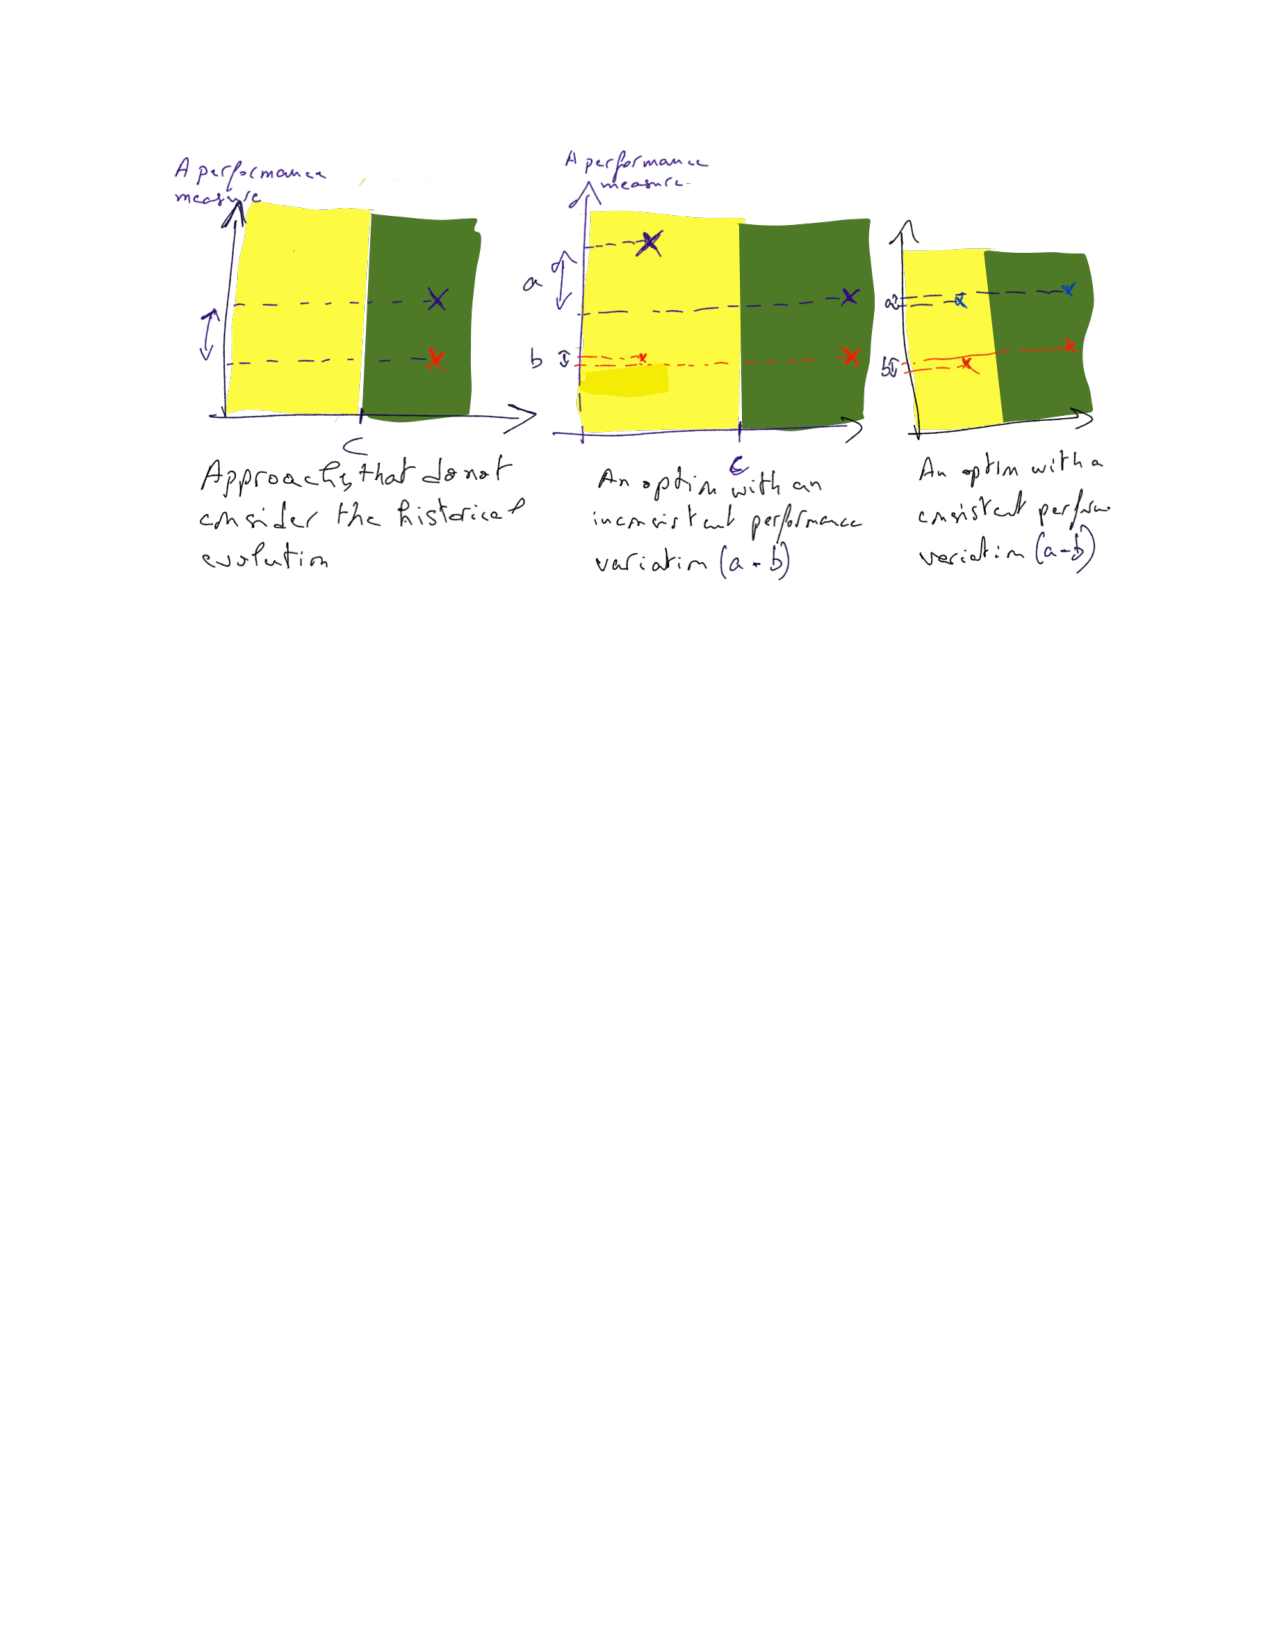
\includegraphics[width=.9\textwidth]{Figures/definition.pdf}
% 		\vspace{-90mm}
% 	\caption{The definition of \inconsistent and how different is it from traditional way of comparing the performance of two values for the same configuration option.\med{todo: label red with v1 and blue with v2}} 
% 	\label{fig:description} 
% \end{figure*}

\begin{figure*}[t]
	\centering
        \begin{subfigure}{0.25\textwidth}
                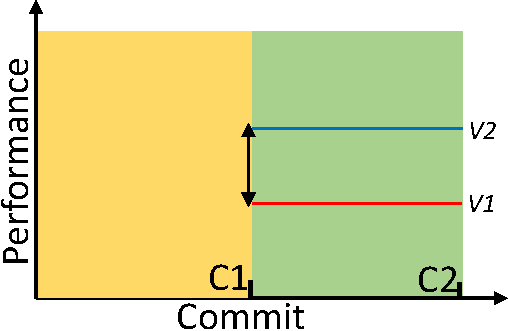
\includegraphics[width=\linewidth]{Figures/background-a.pdf}
                \caption{}
                % \caption{Approaches that donot consider the historical evaluation}
                \label{fig:description-a}
        \end{subfigure}%
        \begin{subfigure}{0.25\textwidth}
                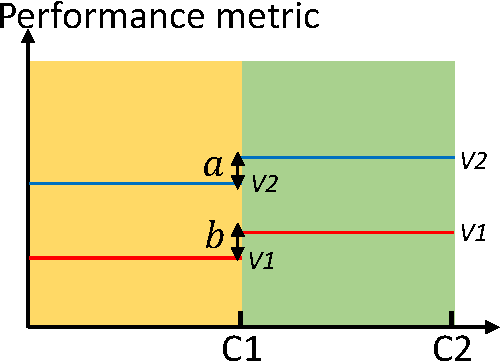
\includegraphics[width=\linewidth]{Figures/background-b.pdf}
                \caption{}
                % \caption{An option with an inconsistent performance variation (a-b).}
                \label{fig:description-b}
        \end{subfigure}%
        \begin{subfigure}{0.25\textwidth}
                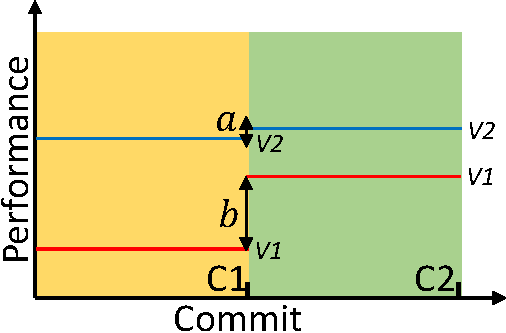
\includegraphics[width=\linewidth]{Figures/background-c.pdf}
                \caption{}
                % \caption{An option with a consistent performance variation (a-b).}
                \label{fig:description-c}
        \end{subfigure}%
        \begin{subfigure}{0.25\textwidth}
                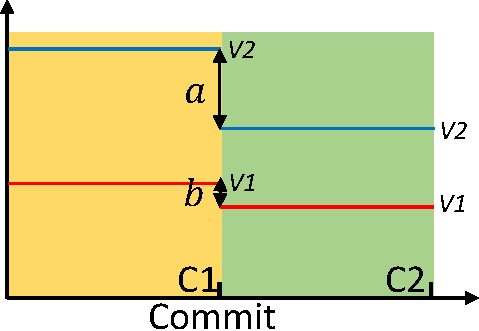
\includegraphics[width=\linewidth]{Figures/background-d.pdf}
                \caption{}
                % \caption{An option with a consistent performance variation (a-b).}
                \label{fig:description-d}
        \end{subfigure}%
	\caption{The definition of \inconsistent and how different is it from traditional way of comparing the performance of two values for the same configuration option: (a) Approaches that do not consider the historical evaluation, (b) An option with an inconsistent performance variation (a-b), (c) An option with a consistent performance variation (a-b), and (d) An option with a inconsistent performance variation (a-b). V1 and V2 are two different values of the same configuration option. C1 and C2 are two revisions. A smaller performance metric value (e.g., cpu usage) indicates a better performance.
	%\heng{(a) ...; (b) ...; (c) ...; (d).... Then explain what is V1, V2, and what is C1, C2. This is to make the figure self-explainable}. 
	%\heng{Make the longer lines just within the green boxes.} 
	%\heng{A smaller performance metric value (e.g., cpu usage) indicates a better performance.}} 
	}
	\label{fig:description}
\end{figure*}


%Furthermore, prior studies do not consider the evolution aspect when configuration performance. 

Traditionally, prior work studied the difference in system performance caused by different values of the same option, without considering how the performance impact of an option evolve due to code changes~\cite{tse}. For instance, traditional approaches compare different values of a configuration option based on their raw performances values~\cite{RN2880,RN3537,RN3543}, as illustrated in Figure~\ref{fig:description-a}. However, such comparison is subjective as
the option's value \emph{V2} with a worse performance might not necessarily be problematic; it might, as an example, just enables the execution of some extra features. Instead, even if an option's value has a good performance compared to other values, it might be significantly different when compared to the performance of the same option value in the prior commit, as shown in the example in Figure~\ref{fig:description-b}. Although the \emph{V2} value has a worse performance, it is much better than the prior commit. Figure~\ref{fig:description-c} shows that both values do not have a large inconsistent performance variation. On the opposite side, an option's value that has a better performance compared to another value of the same option might be facing a large performance regression compared to the prior commit, as shown in the example of Figure~\ref{fig:description-d}. \emph{V1} has a better performance compared to \emph{V2}, but \emph{V1} faces a severe performance regression. 

Therefore, different values of an option can have an inconsistent variation in terms of performance compared to the prior commit. This happens when one or more values of an option exhibit a significant difference compared to the prior release. We refer to such an issue as \textbf{Inconsistent Options Performance Variation (a.k.a, \inconsistent)}. The \inconsistent might be problematic as it can hide a performance regression that is manifested under one configuration option. Similarly, when a default configuration shows an improvement, altering one option's value may indicate no performance improvement or even a performance regression. Such regressions can unfortunately go as unseen to the production environment. 

%In this paper, we instead normalize the performance by considering the prior commit for a tested version. In particular, we measure how much variance exists for an option value between a current version and its prior one. For example, an option X with a value Y in a new commit has a different performance consumption compared to the same option and value prior to the new commit. Then, we study the differences between these last variance to measure if different values for the same option manifest different performances compared to the prior change, which we refer to as ``Inconsistent Options Performance Variation'' (\inconsistent).

%In our prior work~\cite{DBLP:conf/icsm/ChenS17}, we conducted a first step toward assisting practitioners on identifying performance regression at the development stage. In particular, we repetitively execute the existing functional tests or micro-benchmarks for each commit. We identify performance regressions in each test or micro-benchmark if there exists statistically significant degradation with medium or large effect sizes in any performance metric.

In this paper, we perform a case study on two large-scale open-source software systems: \emph{Hadoop} and \emph{Cassandra}. We first conduct a preliminary study to quantify the prevalence of the \inconsistent issue. We observe that 81\% of the commits have at least one option manifesting an \inconsistent issue. We also observe that manually identifying such issues is challenging, as commits do not share the same options that manifest an \inconsistent. That motivates us to propose a automated model that predicts if the combination of a Commit, a Test, and an Option (\textbf{\instance}) would exhibit an \inconsistent issue. We evaluate our prediction model using the following two research questions: 

%Then, we propose a model to predict which Commit, Test, and Configuration (\textbf{\instance}) might suffer from an \inconsistent, which can be harmful. %the impact of software configuration on hiding performance regression and proposed a prediction model to identify such regressions at the development stage. In fact, software configuration makes the identification of performance regression more challenging. 
 %Therefore, we first quantify how often an \inconsistent can occur. Secondly, we propose and evaluate a prediction model that identifies whether a commit has a performance regression that is hidden under a certain configurations. %In particular, a source code change might not always show a regression, but just under certain configurations. Therefore, in this paper, we quantify the impact of software configurations on hiding performance regression. We then propose a prediction model that combines changed source code as well as configuration related metrics to predict whether a commit has a performance regression that might be hidden by a certain configurations. 
%We summarize our contribution in the following three research questions: 

\begin{itemize}
    
    \item \textbf{RQ1. \RQII}
    
    Our prediction model reaches an AUC up to 0.93 and 0.90 for predicting \inconsistent for \emph{Hadoop} and \emph{Cassandra}, respectively. Besides, we observe that random forest is the most performing model for four and three out of five performance measures (i.e., response time, CPU, memory, I/O Read, and I/O write) for \emph{Cassandra} and \emph{Hadoop}, respectively. 
    
    \item\textbf{RQ2. \RQIII}
    
    We observe that all four dimensions of metrics considered in our study, namely the code structure, code change, code token, and configuration options metrics, have a statistically significant impact in predicting \inconsistent. The dimensions that are related to the configuration options and the tokens of the changed code are the most important dimensions for both case studies. 
    
\end{itemize}

\noindent{Paper organization.} The rest of our paper is organized as follows: Section~\ref{sec:back} provides the background information and defines \inconsistent. Section~\ref{sec:relatedwork} provides prior work related to our paper. Section~\ref{sec:datacollection} discusses our approach of conducting experiments and collecting data. Sections~\ref{sec:pq-results} and~\ref{sec:rq-results} present our results. Section~\ref{sec:threats} discusses the threats to the validity o four findings. Finally, Section~\ref{sec:conclusion} concludes the paper. 

\section{Background}
\label{sec:back}


%\subsection{Configuration}

Software configuration is a mechanism used to customize the behaviour of a software system without changing the source code. The configuration \textbf{options} are often stored in configuration files as a set of key - value pairs, where the key represents an option's name and the \textbf{value} represents a default or user-chosen value for that option. We define a \textbf{configuration} as one particular assignment of a value to all existing options. Table~\ref{tab:terms} lists the definition of these terms. For example, \emph{A=1} and \emph{B=2} is one possible configuration for a software system with the two integer options \emph{A} and \emph{B}. Configuration options enable users to adapt the execution of their software systems by simply modifying the values of certain configuration options, without re-compilation. For example, a user can change the directory that stores the cache for \emph{Cassandra} by changing the value of the \textit{saved\_caches\_directory} configuration option.% Such configuration can be changed at run-time without changing or recompiling the source code of the whole software system.

\begin{table}[t]
    \centering
    \caption{Our definition of configuration, option, and value}
    \begin{tabular}{l|p{6.6cm}|l}
        \hline
        Term & Definition & Example \\
        \hline
        \textbf{Option}  & A typed, configurable item that allows users to set different values. & $A$ \\
        \textbf{Value} & A specific assignment of a value for an option. & $A = 1$ \\
        \textbf{Configuration} & An assignment of values to all options by a user. & $A = 1; B = 2$ \\
        \hline
    \end{tabular}
    \label{tab:terms}
\end{table}


Although configuration introduces a large flexibility for users, considering all the possible configurations during testing is impossible. A software system with only three boolean configuration options requires testing 2${^3}$ configurations. In fact, configuration problems are among the dominant \bram{exaggeration (since one of citations is ours)?} problems in software engineering~\cite{tse,RN2897}.

In particular, a software system can suffer from what we refer to as \textbf{Inconsistent Options Performance Variation} (a.k.a, \inconsistent). This occurs when, for a given commit \emph{C}, the performance of a subset of an option's values evolved differently relative to their performance in the commit prior to \emph{C}. Considering the example in Figure~\ref{fig:description}, when comparing the raw performance of the two option values \emph{V1} and \emph{V2} (Figure~\ref{fig:description-a}), we observe that \emph{V1} shows a better performance than \emph{V2}. However, that might not be problematic as \emph{V2} might just enable an extra feature, such as logging a transaction. In fact, in Figure~\ref{fig:description-b} the performance of \emph{V2} is improved compared to the prior commit, while that improvement does not manifest under option value \emph{V1}. \bram{here (and also in intro) we need to argue that this is a more important problem than the first one, but right now this is not entirely convincing/concrete enough} %That indicates the first type of \inconsistent, which consists of an inconsistent improvement across different values of the same option. 
Similarly, Figure~\ref{fig:description-d} shows that even if \emph{V2} does not show any significant performance variation from the prior commit, \emph{V1} suffers from a performance regression. 
A performance variation is calculated as the difference between the performance variation of each option's value after and before each commit, which is illustrated in Figure~\ref{fig:description} by ``$a - b$'' .


%%% Local Variables:
%%% mode: latex
%%% TeX-master: "../main"
%%% End:


\section{Data Collection}
\label{sec:datacollection}
In this section, we %first 
present our subject systems %. Then we present 
and our approach to collect performance regressions and configuration data.% related to system configuration.


\subsection{Subject Systems}
In this paper, we consider %We choose two open-source systems, 
\emph{Hadoop} and \emph{Cassandra} as two %the 
subject systems. % of our case study. 
\emph{Hadoop}~\cite{hadoop2012:White} is a distributed system infrastructure, whereas %. \med{do we need to advertise for hadoop in the following sentence? :)}\emph{Hadoop} performs data processing in a reliable, efficient, high fault tolerance, low cost and scalable manner. 
\emph{Cassandra} is a distributed NoSQL database management system. We choose these two subject systems since their performance is critical for the users and they have been studied in prior research on mining performance data~\cite{markASE,Chen:2014:DPA}. In addition, they have a large number of configuration options. The overview of our subject systems is shown in Table~\ref{tab:subject}.

\begin{table}[htbp]
  \centering
  %\tiny
  \caption{Our studied dataset.}%Overview of our subject systems.}
	\label{tab:subject}
    \begin{tabular}{|c|r|l|r|r|r|}
    \hline
    Subjects & \multicolumn{1}{c|}{\specialcell{\# Studied\\Releases}} & \multicolumn{1}{c|}{Last release} &  \multicolumn{1}{c|}{\# Commits} & \multicolumn{1}{c|}{\specialcell{\# Configuration\\Options}} & \multicolumn{1}{c|}{\# Tests} \\ \hline
    Hadoop & 7     & 2.7.3 & 803 & 365   & 1,853 \\ \hline
    Cassandra & 5     & 3.0.15 & 502 & 162   & 369 \\ \hline
    \end{tabular}
\end{table}


\subsection{Data Gathering}
To answer our research questions, we followed the approach that is summarized in Figure~\ref{fig:overview} and discussed below.
%In the subsection, we describe the pieces of data that we collected in order to answer our research questions. An overview of our data collection process is shown in Figure~\ref{fig:overview}. 

\begin{figure*}[tbh]
	\centering
		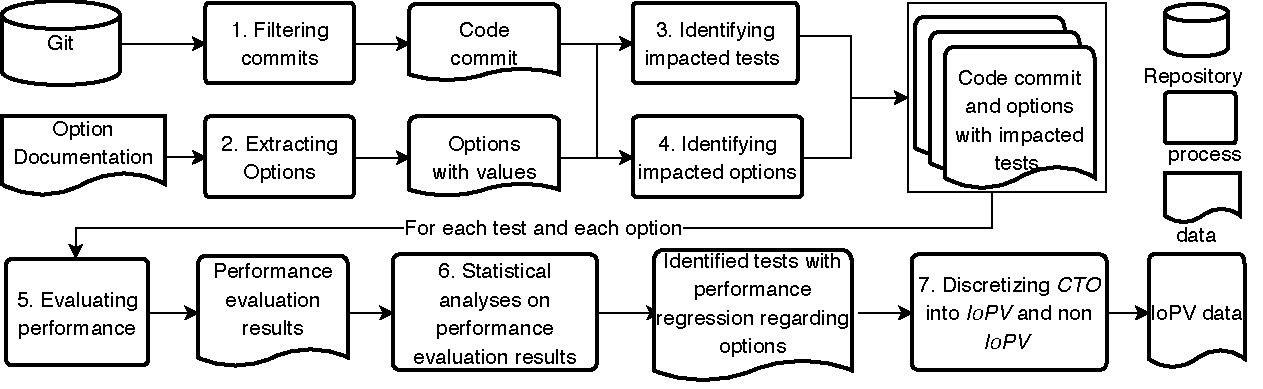
\includegraphics[width=.9\textwidth]{Figures/overview.pdf}
	\caption{An overview of our approach to collect data.} 
	\label{fig:overview} 
\end{figure*}

\subsubsection{Filtering Commits}

Since we study performance variation across different versions of a software system, we only consider source code related changes. In particular, we filter out commits without any \emph{java} source code changes. % after cloning the Git repositories. 
Furthermore, %multiple commits might be associated with the same feature or issue. In particular, 
developers can commit multiple changes toward fixing the same issue, which is defined in the issue tracking system. As \emph{Hadoop} and \emph{Cassandra} use JIRA as a tracking system and have an explicit mapping between commits and issues, we use the issue id mentioned in the commit messages to identify the commits that belong to the same issue. If multiple commits are associated with the same issue, we only consider the last commit. This is important as developers can initially introduce a regression but then fix it before releasing the code changes related to the issue. 


%In the first step, we filter commits that only have source code changes. In particular, we clone our subject systems from Github repository. Then we checkout to each commit and use \emph{git log} command to list all the files that are changed in each commit. In our subject systems, we extract the commits that have source code changes changes to \emph{java} files. To accomplish one development task, multiple commits, including temporary commits, may be made. We would like to avoid considering such temporary commits. Since all our subject systems use JIRA as their issue tracking systems, we use the issue id mentioned in their commit messages to identify commits that belong to the same issue. If multiple commits are associated with the same issue, we only consider the last commit.

\subsubsection{Extracting Options}

In the second step, we extract configuration options and their corresponding values for each subject system (i.e., 355 and 162 configuration options in the last studied releases of \emph{Hadoop} and \emph{Cassandra}, respectively). %There exist hundreds of configuration options in \emph{Hadoop} and \emph{Cassandra}. In particular, there are 355 and 162 configuration options in the last release of \emph{Hadoop} and \emph{Cassandra}, respectively. 
We obtain option names and default values by crawling the documentation of \emph{Hadoop}\footnote{\url{https://hadoop.apache.org/docs/current/hadoop-project-dist/hadoop-common/core-default.xml}} and \emph{Cassandra}\footnote{\url{https://cassandra.apache.org/doc/latest/configuration}} and extracting the configuration file that is shipped with the project's releases. Finally, we manually classified the extracted options based on their expected data types (e.g., Boolean when the default value is \emph{TRUE} or \emph{FALSE}).

%Therefore, to collect all the option names, we develop a crawler in Python to gather options from the official configuration website of \emph{Hadoop} and \emph{Cassandra}\footnote{\url{https://cassandra.apache.org/doc/latest/configuration}}.
%We also extract the type and values of options. For each option, we extract its default value and manually divide its type into boolean, numeric, and enumerated string. 
%For example, if we find that the default value of an option is \emph{FALSE}, we consider the type of such option to be boolean. 

\subsubsection{Identifying Impacted Tests}
\label{sec:impactedtests}
We automatically create a mapping between the changed source code in each commit and the existing unit tests. %%a mapping between the existing unit tests and %correspondingly 
%the changed source code for that commit. 
We derive such commit-test mapping based on the automatically generated method-level code coverage results, similarly to our prior study~\cite{jinfu_tse2020}. 
%\med{I see that the two sentences that describe the approach are commented, it looks like we are asking readers to read 2 papers to understand our approach. I still think that we should put it back}
%for each commit all the changed methods % by adding invocation to logging libraries 
%and run all the exiting unit tests. The tests that run the instrumented source code are the test that are associated with a commit's change. 
%\heng{Check if the following is right: } 
For each commit, we automatically add logging instrumentation to each  method, which will print log messages that indicate the execution of the method at runtime\footnote{Note that the instrumented versions are only used to identify impacted tests and options, and they are not used in our actual performance valuation.}.
We then run each test for the commit. A test is considered impacted by the commit if any instrumented logging is outputted.
Afterwards, we only run the tests that execute the changed source code for a given commit since executing all the existing tests of a software system for each commit and each possible configuration is practically infeasible. In addition, running those tests that are not impacted by the code change of a commit is not likely to detect performance variations (regressions or improvements under some values of an option). 

%in every version of the source code of our subject systems by adding invocation to logging libraries. We run all the available tests of each released version of the subject systems. By analyzing the output of our instrumentation, we obtain a list of methods that are executed during the running of each test. Then, we can create mappings between each test and the executed methods of the test. With such a mapping between tests and methods in the source code, for each commit, we can identify the tests that are likely to be impacted by identifying the methods that are changed in the commit, i.e., a method-to-test mapping for each commit. Due to the resources needed for creating such mappings, we only update such mappings for every release of the subject systems.

%We consider using all the functional test that exist in the repository. We use these tests since these tests are maintained and typically executed regularly during every build in the release pipeline of software development~\cite{DBLP:journals/software/TillmannS06}. Not all the tests are impacted by the code changes and options in a commit and running those un-impacted tests is not likely to detect performance regressions. 

%To identify all the impacted tests by each commit, we create mappings between source code and tests. We automatically instrument all the methods in every version of the source code of our subject systems by adding invocation to logging libraries. We run all the available tests of each released version of the subject systems. By analyzing the output of our instrumentation, we obtain a list of methods that are executed during the running of each test. Then, we can create mappings between each test and the executed methods of the test. With such a mapping between tests and methods in the source code, for each commit, we can identify the tests that are likely to be impacted by identifying the methods that are changed in the commit, i.e., a method-to-test mapping for each commit. Due to the resources needed for creating such mappings, we only update such mappings for every release of the subject systems.

\subsubsection{Identifying Impacted Options}% \heng{Identifying Impacted Options?}}
Similarly to identifying which tests to run for a given commit, we also select which configuration options to change when running each of these last tests. To do so, we first identify how \emph{Hadoop} and \emph{Cassandra} access the value of a configuration option by searching for option names in the source code files. We found that all the options are accessible via \emph{getters} that are defined in one class provider (e.g., \emph{DatabaseDescriptor.java}\footnote{\url{https://github.com/apache/cassandra/blob/trunk/src/java/org/apache/cassandra/config/DatabaseDescriptor.java}} to access the \emph{Cassandra}'s options). Second, we identify the methods that invoke these configuration options' \emph{getters}. Finally, we dynamically identify which of these methods are executed when running a test similarly to the approach discussed in Section~\ref{sec:impactedtests}. If any method that can access an option is executed, the option is considered impacted by the commit.

%In this step, we identify the methods which call the options in direct or indirect ways. We call such methods impacted methods. We first extract the methods that call the options directly. We call such methods direct-call-method. To extract such direct-call-method, we follow a heuristic approach to find the methods that contain configuration names. In particular, we use ``grep -r option\_name *" to search all the methods that contain the option names in the path of each subject system. With the returned methods, we manually filter and determine the direct-call-methods. In our subject systems, we find that all the direct-call-methods are in the same \emph{Java} class file. For example, all the direct-call-methods are in the class named \emph{DatabaseDescriptor.java}\footnote{\url{https://github.com/apache/cassandra/blob/trunk/src/java/org/apache/cassandra/config/DatabaseDescriptor.java}}.

%Second, we extract the methods that call the direct-call-method. We iterate all the methods from the method-to-test mapping generated in last subsection, to find the methods that call the direct-call-method. Finally, based on the mapping between options and impacted methods, with mapping between methods and tests, we can generate the methods and tests impacted by each option.

\subsubsection{Evaluating Performance}
\label{evaluation}
After obtaining which tests and which options are impacted by each commit, we exercise the test on each commit and its parent commit (i.e., the previous commit) to evaluate their respective performances. %For each test, 
We first execute each test with all the configuration options set at their default values. Then we alter the value of one configuration option at a time. For the configuration options with boolean values, we alter the configuration option to the value that is not the default. For example, if the default value is \emph{TRUE}, we would alter the value to be \emph{FALSE}. For numeric type option, we alter the configuration option to the value of the double of the default value and half of the default value. For example, if a configuration option has a default value of $100$, we would run the test with altering the value to $200$ and then run the same test with altering the value to $50$. %\ian{I don't understand the next sentence.\med{is it better now?}}
We alter to each of the possible values for the enumerate type options. %For enumerated string type option, we execute the same test multiple times, each of which with one of the existing enumerated string values. %Note that we do not execute the tests with the instrumented source code that we discussed in Section~\ref{sec:impactedtests}. 

%We exercise the selected tests with different configurations of each pair of current and parent commits to evaluate their performance. In particular, we execute the same tests with same configuration option in different option values. In terms of different option values, for boolean type option, we execute the same test with \emph{TRUE} and \emph{FALSE} values. For numeric type option, we exetute the test with \emph{default}, 2*\emph{default}, and \emph{default}/2 values. For enumerated string type option, we execute the same test with all the existing enumerated string values.

Our performance evaluation environment is based on Google Compute Engine~\footnote{\url{https://cloud.google.com/compute}} with 8GB memory and 16 cores CPU. In order to generate statistically rigorous performance results, we adopt the practice of repetitive measurements~\cite{peterfse} to evaluate performance. Conservatively, we executed each test 30 times independently, which is larger than prior work that  %since prior research often only 
repeat a test only 5 to 20 times~\cite{Laaber2018MSR, Leitner2016TIT,DBLP:journals/ese/LaaberSL19}. 

To measure the performance that is associated with each test, we %catch the process of each test and 
use a performance monitoring tool named \emph{psutil}~\footnote{\url{https://github.com/giampaolo/psutil}} (Python system and process utilities). % to capture performance data of such process.
\emph{Psutil} can capture detailed performance metrics and has been widely used in prior research~\cite{DBLP:conf/icsm/ChenS17,DBLP:conf/wosp/YaoPSSTS18}. We collect both domain level and physical level performance metrics. In our execution, we collect five performance metrics during the execution, including response time, CPU usage, memory usage, I/O read and I/O write.

The entire data collection process took around 12,536 machine-hours.

\subsubsection{Statistical Analyses on Performance Evaluation Results}
\label{sec:statisticalAnalysis}

To identify the \inconsistent, we statistically compare the performance of a given test and a configuration option value before and after each commit using the %We perform statistical analyses on the performance data from each pair of current and parent commits to determine the existence and the magnitude of performance regression in a statistically rigorous manner. 
%We use 
Mann-Whitney U test~\cite{nachar2008mann} %to examine if there exist statistically significant differences 
(i.e., $\alpha$ $=$ 0.05) and Cliff\textquotesingle s delta~\cite{ES2006:Becker} that measures the magnitude of performance regressions. We choose Mann-Whitney U test since it does not have any assumption on the distribution of the data. Researchers have shown that reporting only the statistical significance may lead to erroneous results (i.e., if the sample size is very large, p-value can indicate statistical significance even if the difference is trivial). Thus, we also use Cliff\textquotesingle s delta to quantify the magnitude of the differences (a.k.a., effect sizes). Cliff\textquotesingle s delta measures the effect size statistically and has been used in prior engineering studies~\cite{ICSE2002:Kitchenham, Liao2020LogPerfReg, DBLP:journals/ese/LiCSH18}. Cliff\textquotesingle s delta ranges from -1 to +1, where a value of 0 indicates two identical distributions. Therefore, each commit, test, and option's value has a Cliff\textquotesingle s delta value. We then calculate the differences between the maximum and minimum Cliff\textquotesingle s delta for an option's different values, which we used later on to discretize a commit, test, and option as an \inconsistent or a non \inconsistent, as discussed in the following paragraph.

We also measure whether a test manifesting a performance regression when the value of the effect size is positive and indicate medium ($0.33 <$ \emph{Cliff\textquotesingle s delta} $\leqslant 0.474$) or large ($0.474 < $\emph{Cliff\textquotesingle s delta}) magnitude. On the other hand, we consider a test manifesting a performance improvement if the value of the effect size is negative and indicate medium ($-0.33 <$ \emph{Cliff\textquotesingle s delta} $\leqslant -0.474$) or large ($-0.474 > $\emph{Cliff\textquotesingle s delta}) magnitude. 


Note that we consider this statistical analysis for each performance metric (i.e., response time, CPU usage, memory usage, I/O read and I/O write) separately. For example, a commit may show a CPU regression or improvement, but does not show any differences for the response time. 

%Based on the statistical analysis results, each commit is labelled with five different performance metrics (i.e., response time, CPU usage, memory usage, I/O read and I/O write) that are collected during the execution of the test. For example, the CPU label indicates whether the test demonstrate performance regression in terms of CPU usage. \ian{needs to say both regression and improvement}


\subsubsection{Discretizing \instance into \inconsistent and non \inconsistent}
\label{sec:discretizing}
In the final step, we categorize each commit, test, and option (\instance) into a \inconsistent or a non \inconsistent %the maximum difference values into \emph{small} and \emph{large} differences 
based on an automatically determined threshold. Our intuition is that the maximum difference values would be concentrated in either small values (i.e., when adjusting a option does not make a difference) or large values (i.e., when adjusting a option does make a difference), which is demonstrated in Figure~\ref{fig:description}. % using the real data from Hadoop version. 
Specifically, we use Ckmeans.1d.dp~\cite{Ckmeans138:online}, a one-dimensional clustering method, to find a threshold that separates the maximum difference values into two groups, i.e., \inconsistent and a non \inconsistent (see Figure~\ref{fig:threshold_hadoop} and ~\ref{fig:threshold_cassandra}). Note that the option variation range between 0 when there is no variation and 2 when the effect size (c.f. Section~\ref{sec:statisticalAnalysis}) is 1 for one option value and -1 for another value of the same option. Most of the automatically obtained thresholds are close to 1. That indicates, as an example, that one option value might show a large performance effect size compared to the prior commit, while another value for the same option does not show any difference from the prior commit (effect size equals to 0). A second example is when one option's value show a large performance improvement over the prior commit (effect size equals to -1), when another value of the same option does not show any statistically significant difference (effect size equals to 0).
%The categorized difference values (i.e., \emph{small} or \emph{large}) is our target variable.

\begin{figure}[t]
	\centering
        \begin{subfigure}{0.19\textwidth}
                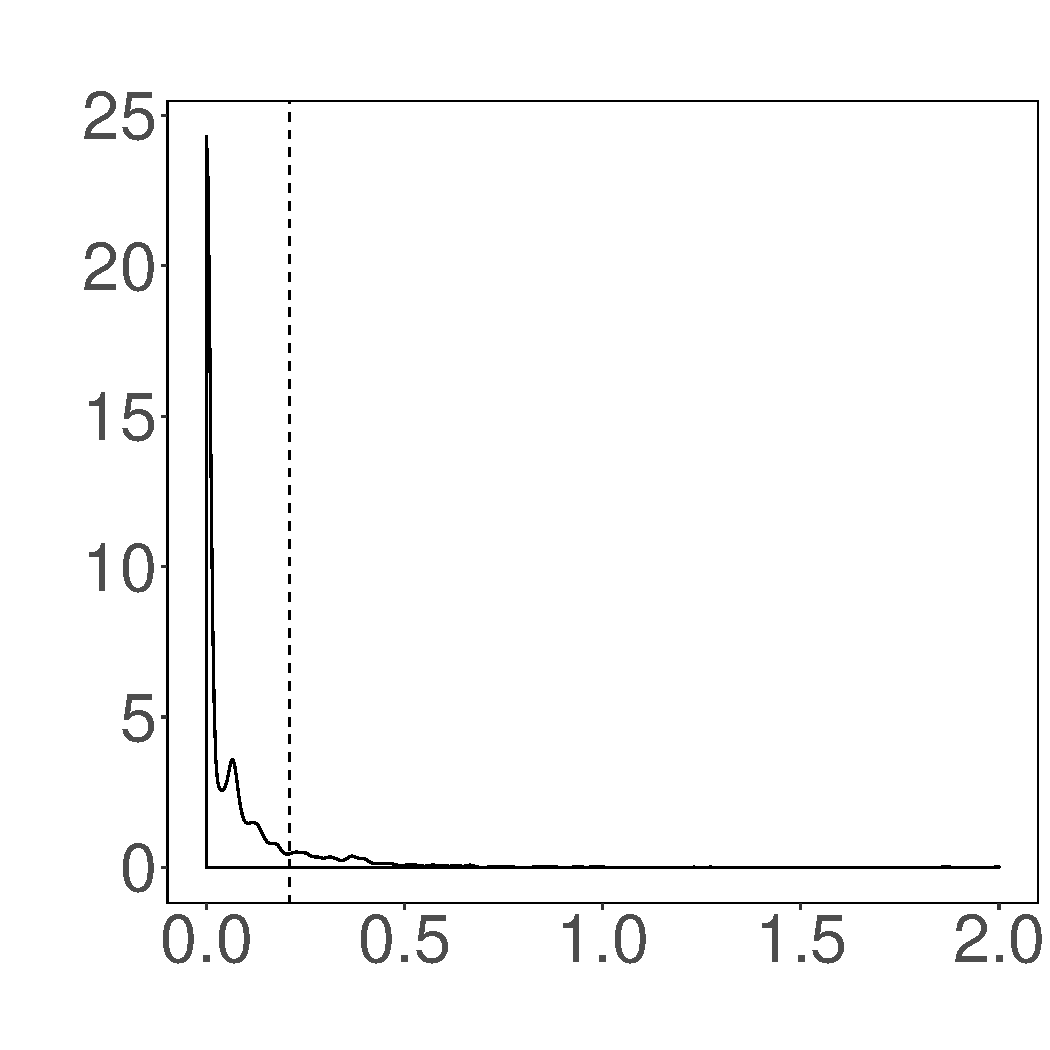
\includegraphics[width=\linewidth]{Figures/runtime-hadoop-cluster.pdf}
                \caption{Res. time}
        \end{subfigure}%
        \begin{subfigure}{0.19\textwidth}
                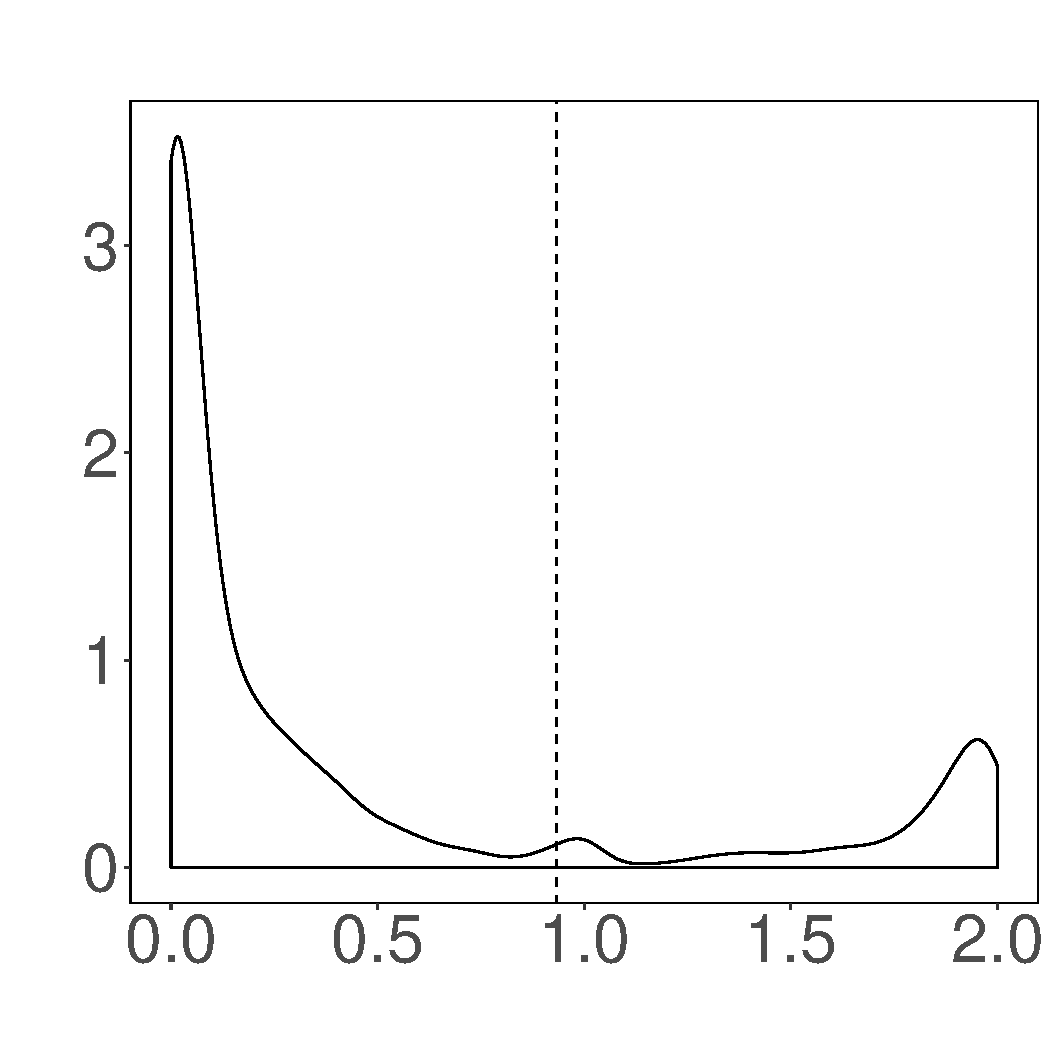
\includegraphics[width=\linewidth]{Figures/cpu-hadoop-cluster.pdf}
                \caption{CPU}
        \end{subfigure}%
        \begin{subfigure}{0.19\textwidth}
                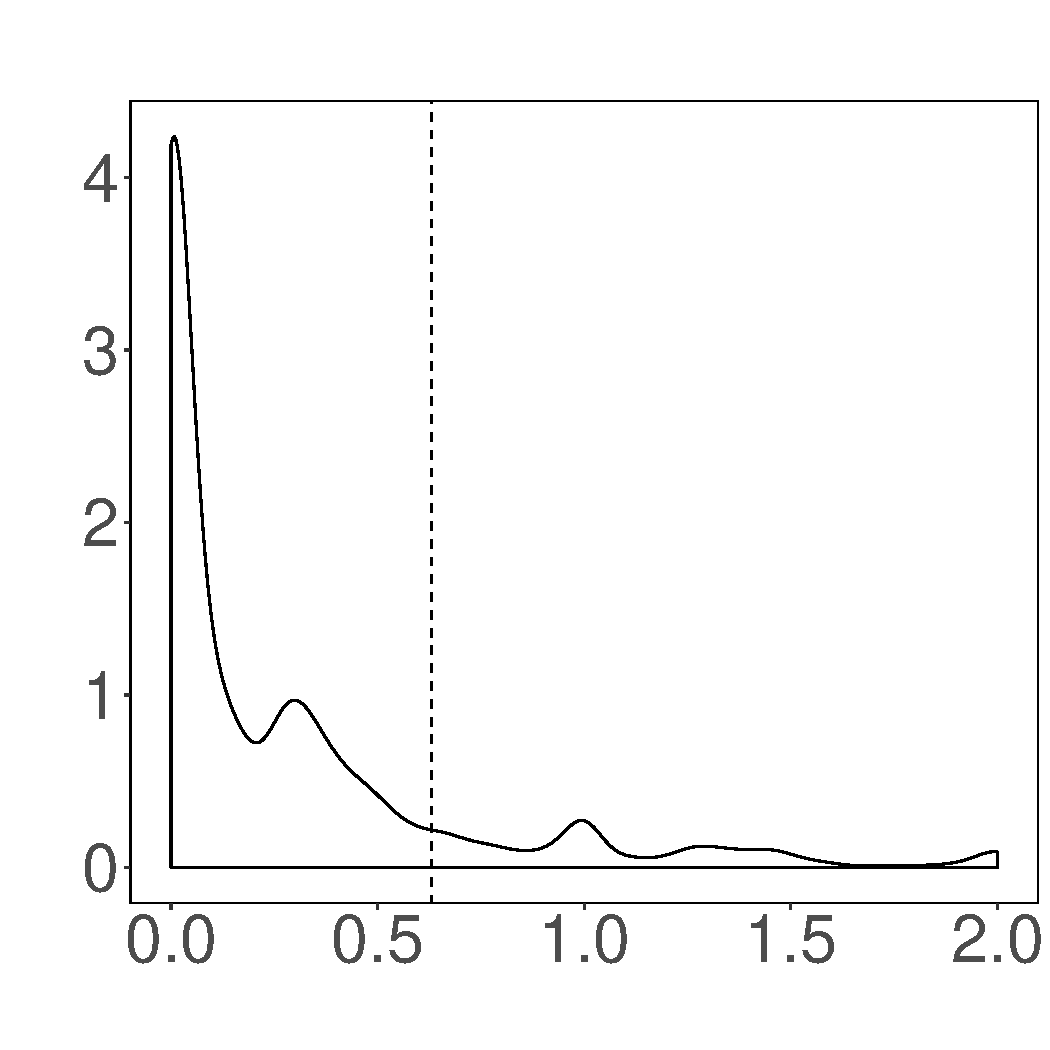
\includegraphics[width=\linewidth]{Figures/mem-hadoop-cluster.pdf}
                \caption{Memory}
        \end{subfigure}%
        \begin{subfigure}{0.19\textwidth}
                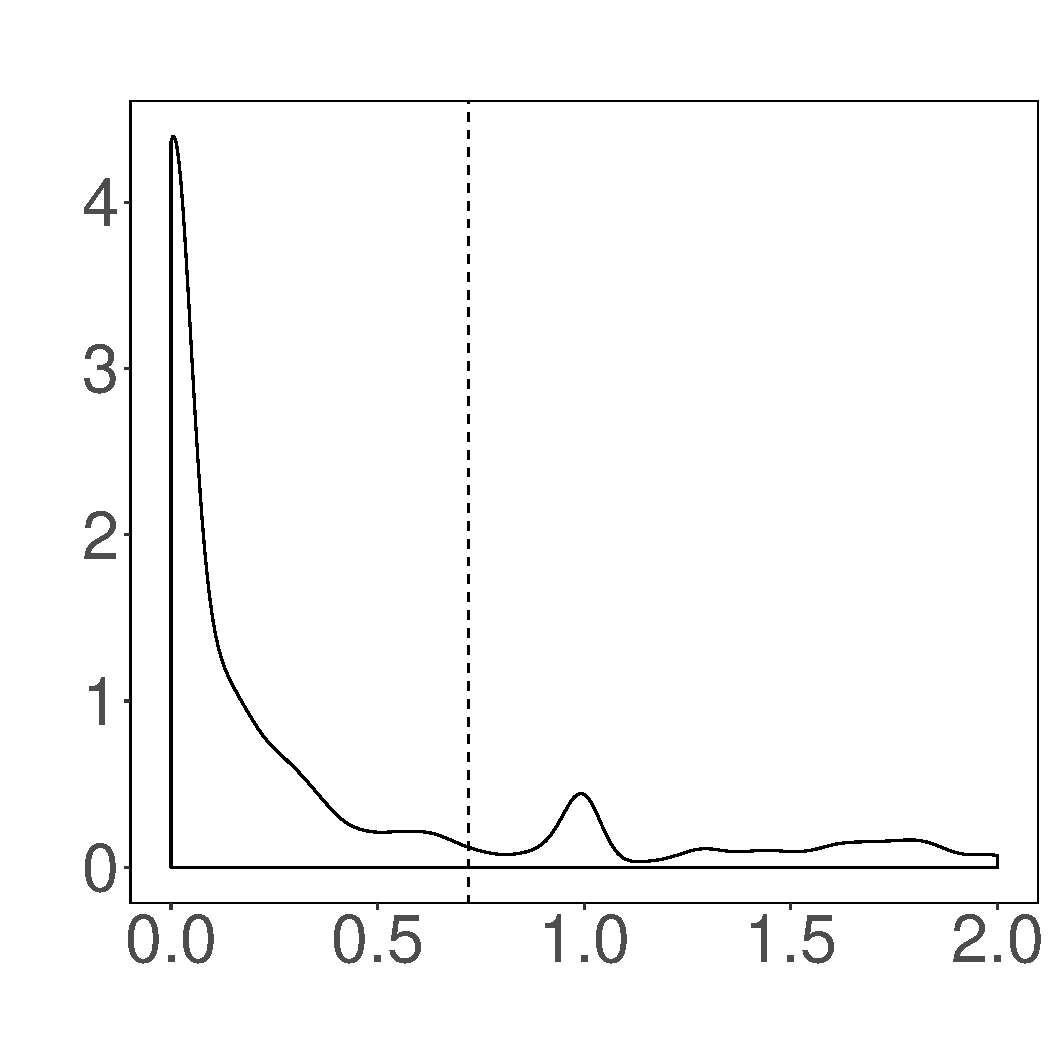
\includegraphics[width=\linewidth]{Figures/ioread-hadoop-cluster.pdf}
                \caption{I/O read}
        \end{subfigure}
        \begin{subfigure}{0.19\textwidth}
                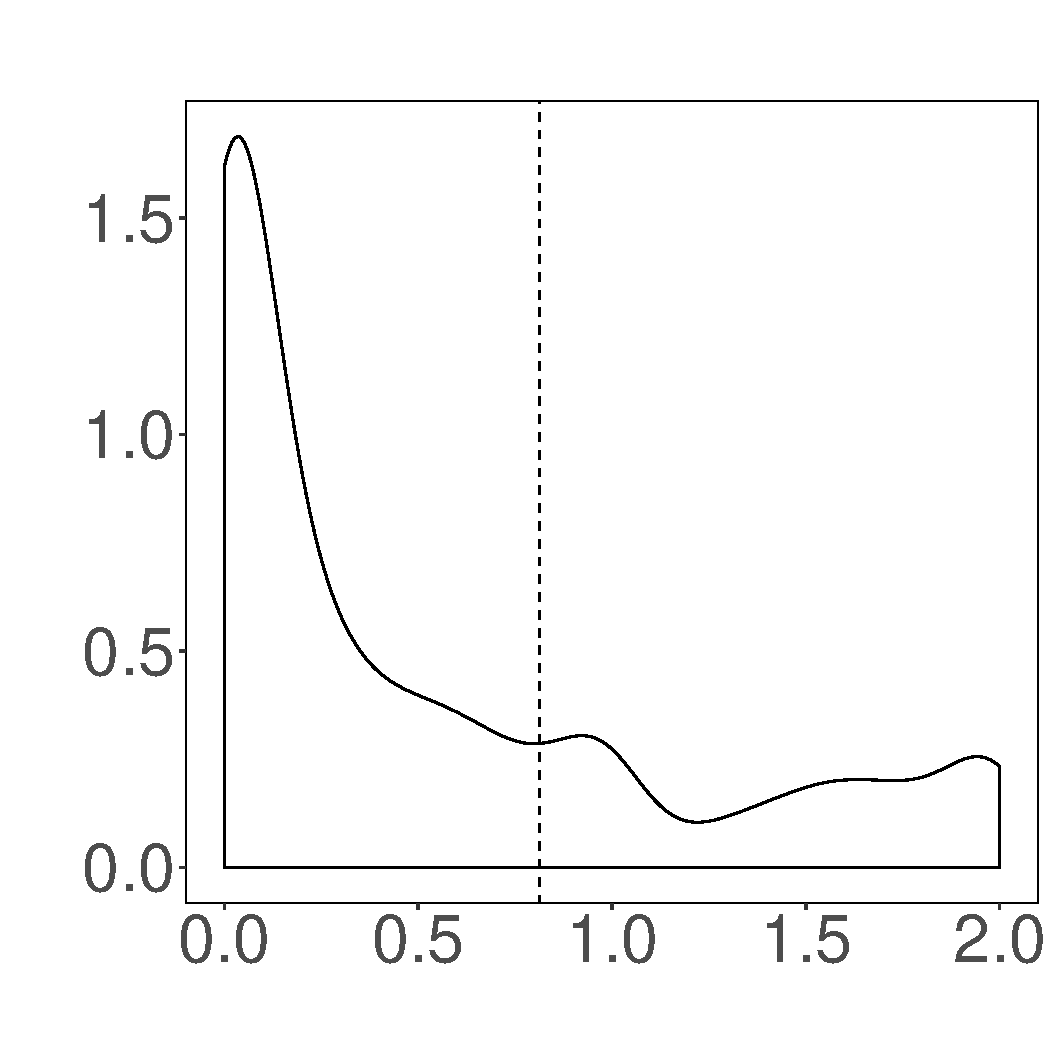
\includegraphics[width=\linewidth]{Figures/iowrite-hadoop-cluster.pdf}
                \caption{I/O write}
        \end{subfigure}
        
	\caption{The automatically obtained threshold for splitting option variation into \inconsistent and non-\inconsistent groups for \emph{Hadoop}.} % \med{Canssadra or Hadoop? Both fig. 3 and fig. 4 showed Hadoop}.}
	\label{fig:threshold_hadoop}
% 	\vspace{-0.15cm}
\end{figure}

\begin{figure}[t]
	\centering
        \begin{subfigure}{0.19\textwidth}
                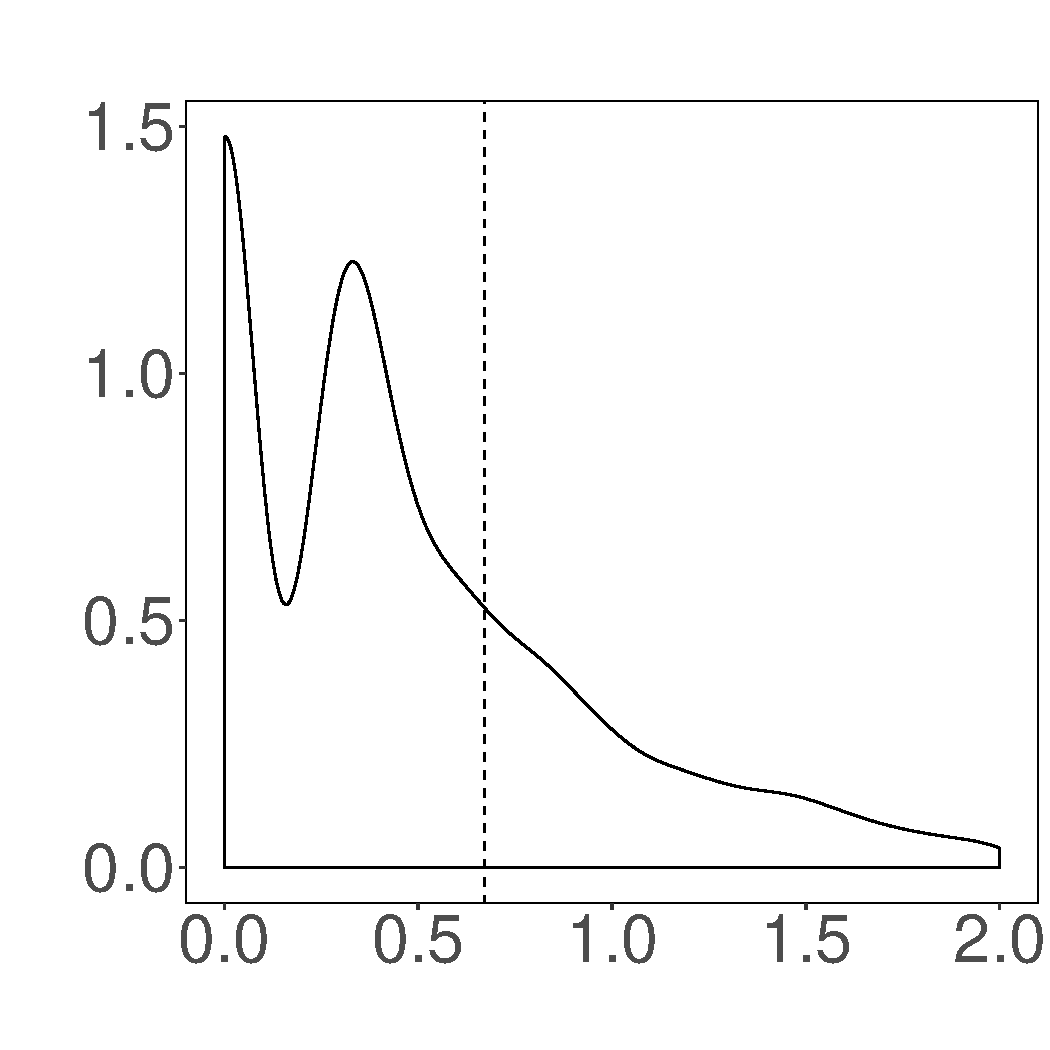
\includegraphics[width=\linewidth]{Figures/runtime-cassandra-cluster.pdf}
                \caption{Res. time}
        \end{subfigure}%
        \begin{subfigure}{0.19\textwidth}
                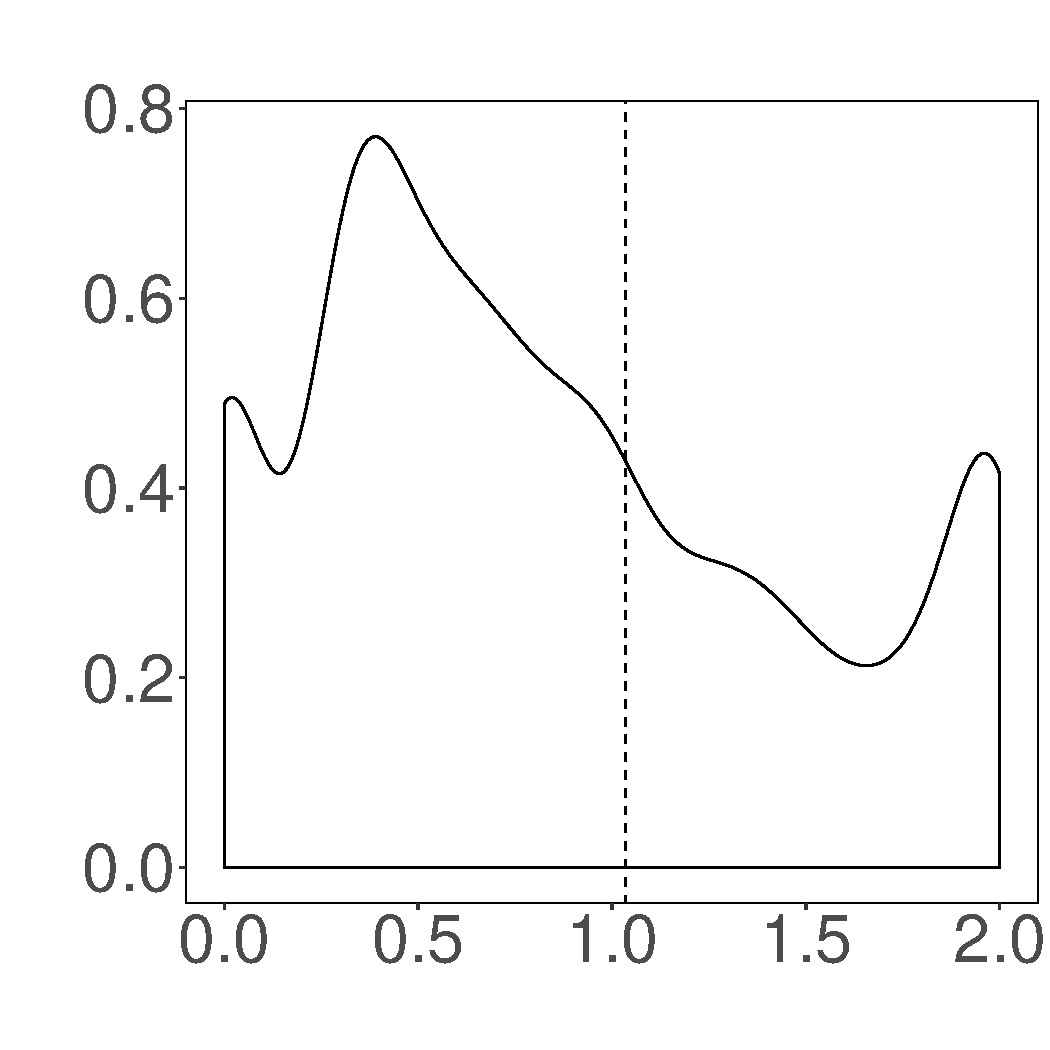
\includegraphics[width=\linewidth]{Figures/cpu-cassandra-cluster.pdf}
                \caption{CPU}
        \end{subfigure}%
        \begin{subfigure}{0.19\textwidth}
                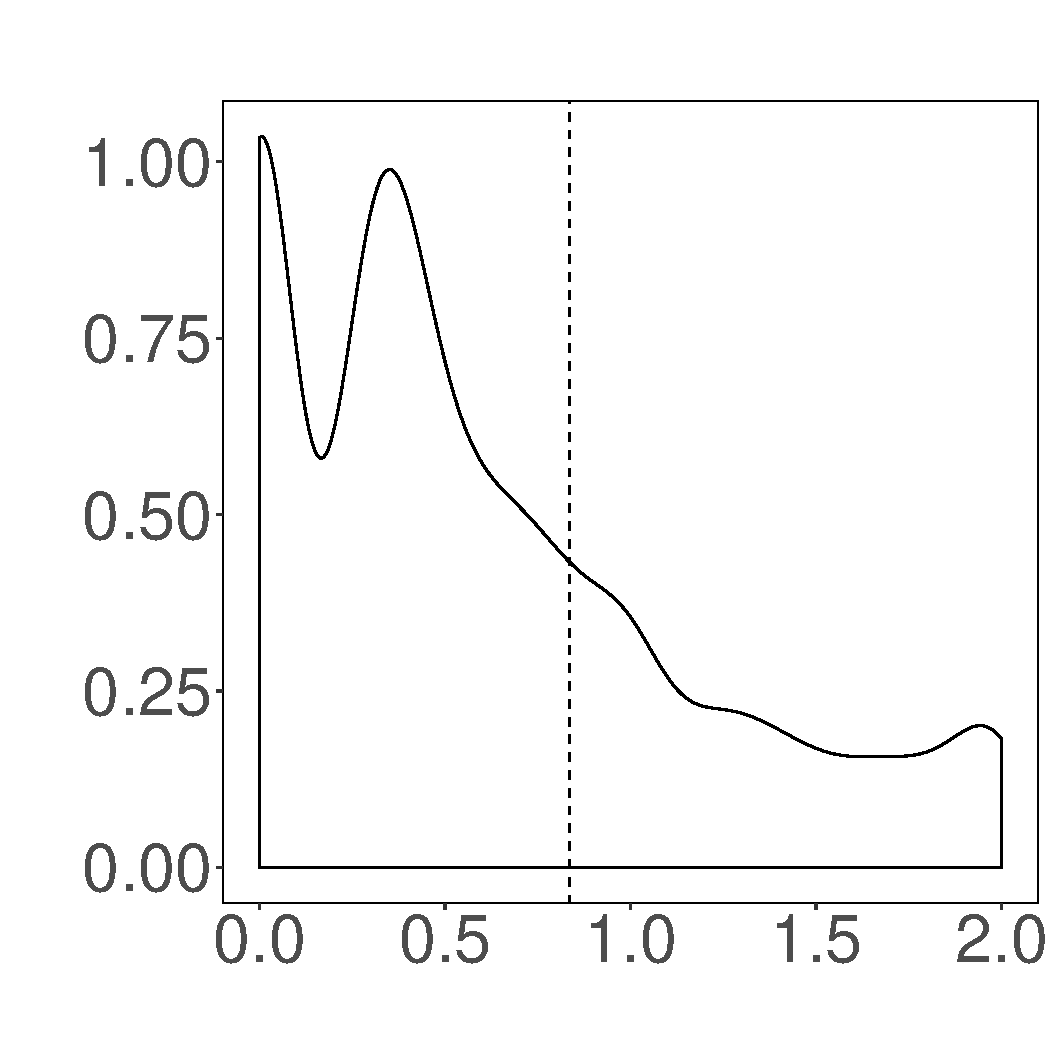
\includegraphics[width=\linewidth]{Figures/mem-cassandra-cluster.pdf}
                \caption{Memory}
        \end{subfigure}%
        \begin{subfigure}{0.19\textwidth}
                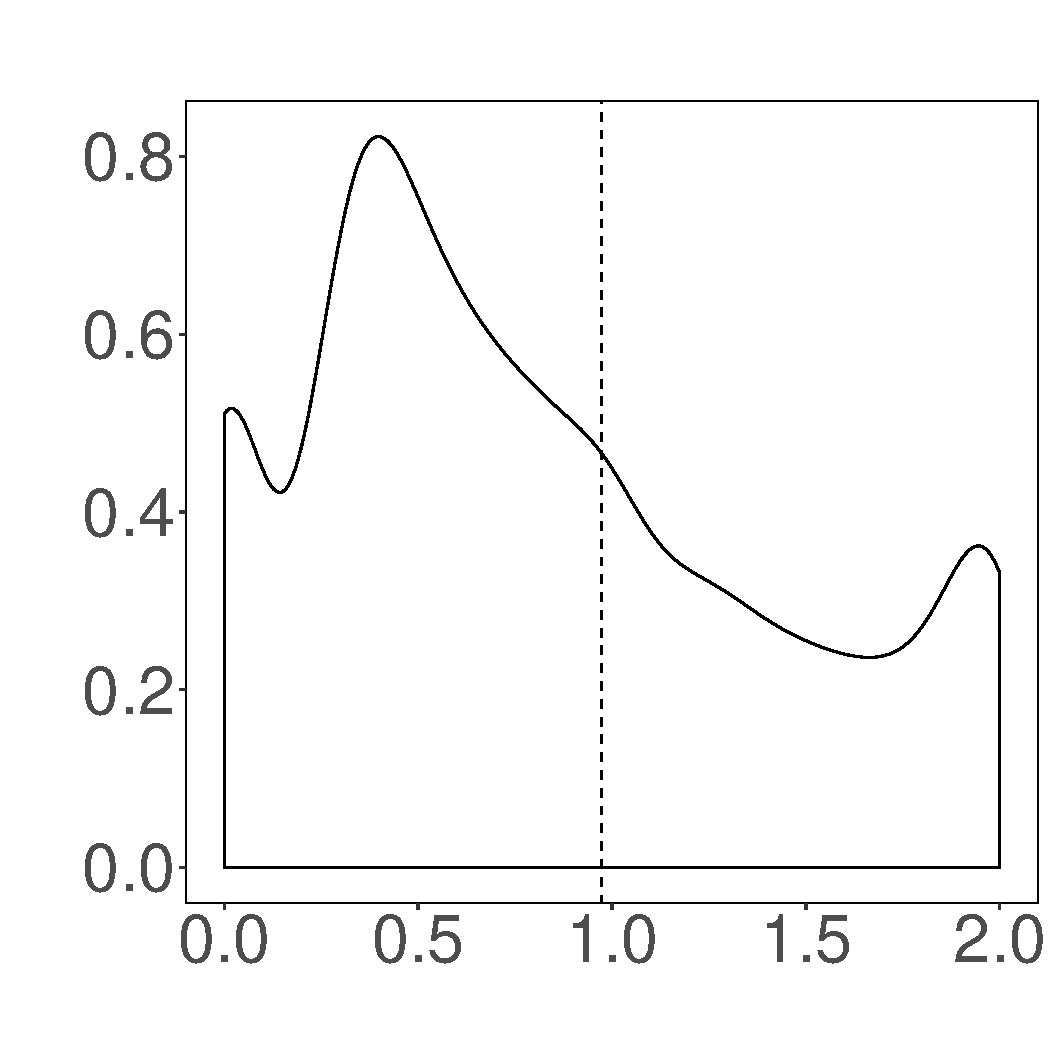
\includegraphics[width=\linewidth]{Figures/ioread-cassandra-cluster.pdf}
                \caption{I/O read}
        \end{subfigure}
        \begin{subfigure}{0.19\textwidth}
                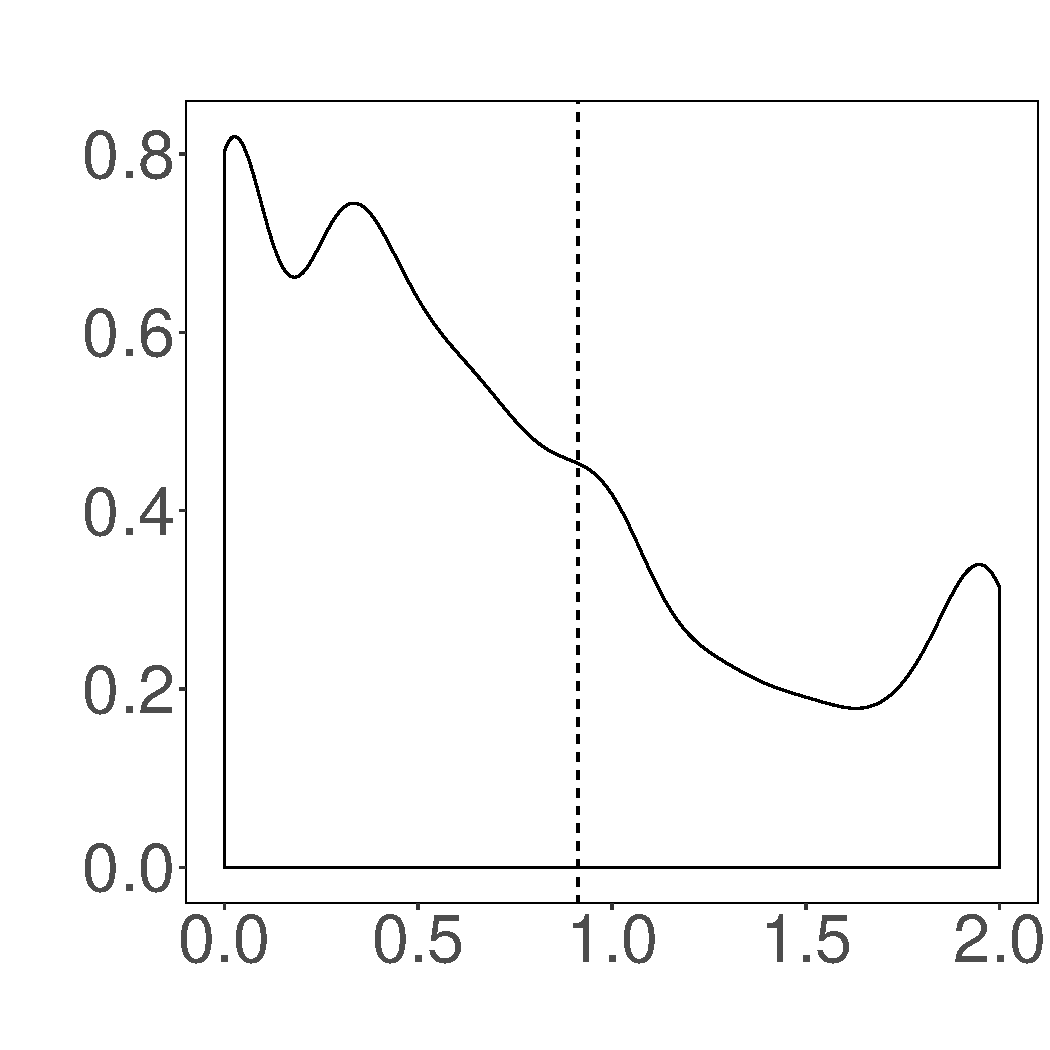
\includegraphics[width=\linewidth]{Figures/iowrite-cassandra-cluster.pdf}
                \caption{I/O write}
        \end{subfigure}
        
	\caption{The automatically obtained threshold for splitting option variation into \inconsistent and non-\inconsistent groups for \emph{Cassandra}.} % \med{Canssadra or Hadoop? Both fig. 3 and fig. 4 showed Hadoop}.}
	\label{fig:threshold_cassandra}
% 	\vspace{-0.15cm}
\end{figure}


%\section{Results}
%\label{sec:results}
%In this section, we present the results in order to answer our three research questions. For each research question, we present the motivation of the questions, the approach that we use to answer the question and its corresponding results. 

\section{Preliminary Study: Quantifying the Prevalence of \inconsistent and the Challenge of Identifying \inconsistent } \label{sec:pq-results}

This preliminary study will shed light on the problem of \inconsistent, which can be further explored by future work. We quantify, through this preliminary study, the existence of the \inconsistent problem in large and highly configurable software systems, as well as how difficult is it to identify the \inconsistent. 
This preliminary analysis will also motivate the need for an approach that automatically identifies the \inconsistent. 
In particular, we address the following preliminary research questions: 

\begin{itemize}
    \item[] PQ1: \PQI
    \item[] PQ2: \PQII
\end{itemize}

\subsection*{\textbf{PQ1. \PQI}}
\label{sec:rq1}
\subsubsection*{Motivation}
The goal of this preliminary research question is to quantify and provide scientific evidences on how often a configuration option can suffer from the \inconsistent issue. %impact that different configurations can have on the manifestation of performance regression. %on Prior research has reported that configuration has an significant relationship to performance~\cite{}. 
%Improper configuration option may cause performance bug and lead to monetary loss. However, little knowledge about the impact of configuration options on the performance regression. %Therefore, in this research question, we would like to study the impact of configuration option on manifestations of performance regressions.
While a new code change might not show any performance regression under the default configuration, another configuration can hide a performance regression that can go as unseen to the production environment. This is an important problem as performance issues often lead to serious monetary losses\footnote{\url{https://www.eweek.com/networking/it-outages-cause-businesses-26.5-billion-in-lost-revenue-each-year-survey}}. similarly, a configuration improvement might not be manifested under all the configurations.  %Therefore, in this research question, we quantify and provide scientific evidences on how often a configuration option can suffer 

%a performance regression can be manifested under one or a subset of the possible configurations.
 
\subsubsection*{Approach}
To quantify the prevalence of \inconsistent, we followed the approach discussed in Section~\ref{sec:datacollection} to collect the performance data. In particular, we first collect performance measurements for each commit, test, and option (which we refer to as \textbf{\instance}) and label each \instance as \inconsistent or a non \inconsistent. %by following the data collection and discretization approach of Section~\ref{sec:datacollection}. In other words, we label each commit, test, and option as \inconsistent or a non \inconsistent. %\textbf{Note that each CTC has one option's value that is different from the default configuration. }
%In addition, to better understand the impact of \inconsistent, 
Then, we identify for each commit and unit test the number of configurations under which the performance is statistically significantly worse (aka, performance regression) or better (aka, performance improvement) than the performance of the same test and configuration in the prior commit. Finally, we quantify for each commit the number of tests that show a performance regression or a performance improvement under just a subset of the existing configurations. 
In the studied \emph{Hadoop} and \emph{Cassandra} releases, there are 4,902 and 4,197 \instance, respectively. 


%\bram{do we need this first paragraph here? seems to repeat general approach?\med{I rewrite this paragraph in the first paragraph above and comment the old paragraph}}
%In order to measure the impact of configuration on the manifestations of performance regressions, for each configuration option, we vary the value while keep all other configuration options at their default values. With each configuration option value, we measure for each test, whether there exists a performance regression, a performance improvement or neither. We would like to see to what extend there exist the cases where one configuration option value leads to performance regression while the another configuration option value leads to a performance improvement or with no change. More importantly, we are in particular interested in the cases where with the default configuration option, the performance has no significant changes or with improvement; while other configuration option leads to performance regression. Such cases would be extremely impactful in practice when the potential performance regressions are unawared by practitioners. 


\subsubsection*{Result}

\noindent \textbf{The \inconsistent is a common problem, as 61\% and 91\% of our studied \instance in \emph{Hadoop} and \emph{Cassandra} suffer from the \inconsistent problem.} In addition, each \emph{Hadoop} and \emph{Cassandra} commit has a median percentage of 43\% and 96\% of the tests and options that manifest at least one \inconsistent, as further detailed in Figure~\ref{fig:iopv_per_commit_hadoop} and~\ref{fig:iopv_per_commit_cassandra}. Although only a small percentage of \emph{Hadoop} tests and options suffers from an \inconsistent in terms of response time, the other performance metrics show a large percentage of tests and options that suffer form \inconsistent, as shown in Figure~\ref{fig:iopv_per_commit_hadoop}. On the other hand, the percentage of tests and options that suffer from an \inconsistent is larger than the tests and options that do not face an \inconsistent for \emph{Cassandra} across all the performance metrics, as shown in Figure~\ref{fig:iopv_per_commit_cassandra}.  % show the results about the percentage of test and options in each commit that suffer from \inconsistent forf each performance measure. %\med{add 5 figures, each of which is with 2 boxplots. One boxplot shows the \% of \inconsistent in each commit and the other boxplot shows the \% of the non \inconsistent}. \med{a sentence about the new figures}.  
%\med{how often the (max-min) is large, medium, ...? Need a table like table 2 for that, or is it the 3rd sub table in Table 2? } \jinfu{We use one dimension cluster to group the (max-in). Therefore, the diff of effect size (i.e., max-min) exist no large and medium}
%Another comment, can you split Table 2 to 3 tables? \jinfu{splitted}}

\begin{figure}[t]
	\centering
        \begin{subfigure}{0.19\textwidth}
                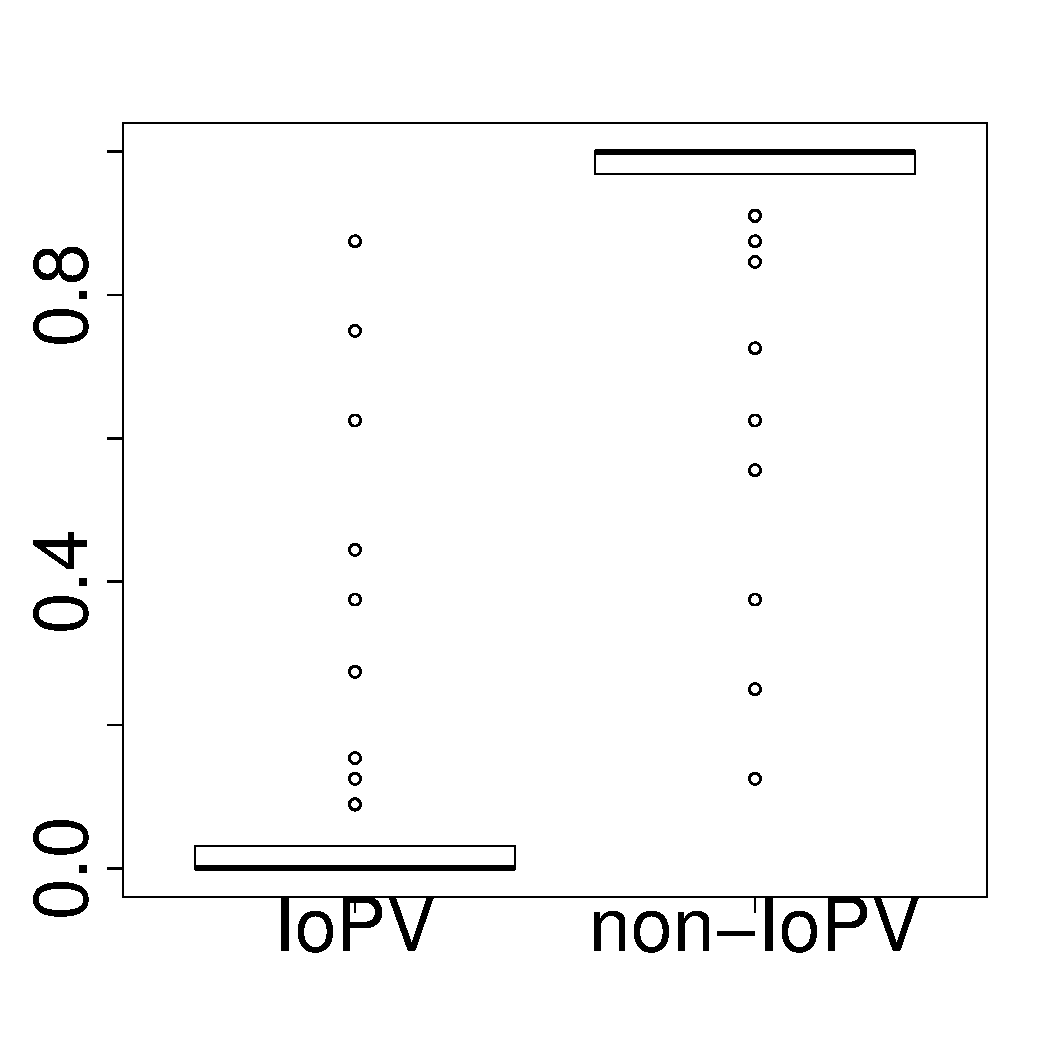
\includegraphics[width=\linewidth]{Figures/runtime-hadoop-boxplot.pdf}
                \caption{Res. time}
        \end{subfigure}%
        \begin{subfigure}{0.19\textwidth}
                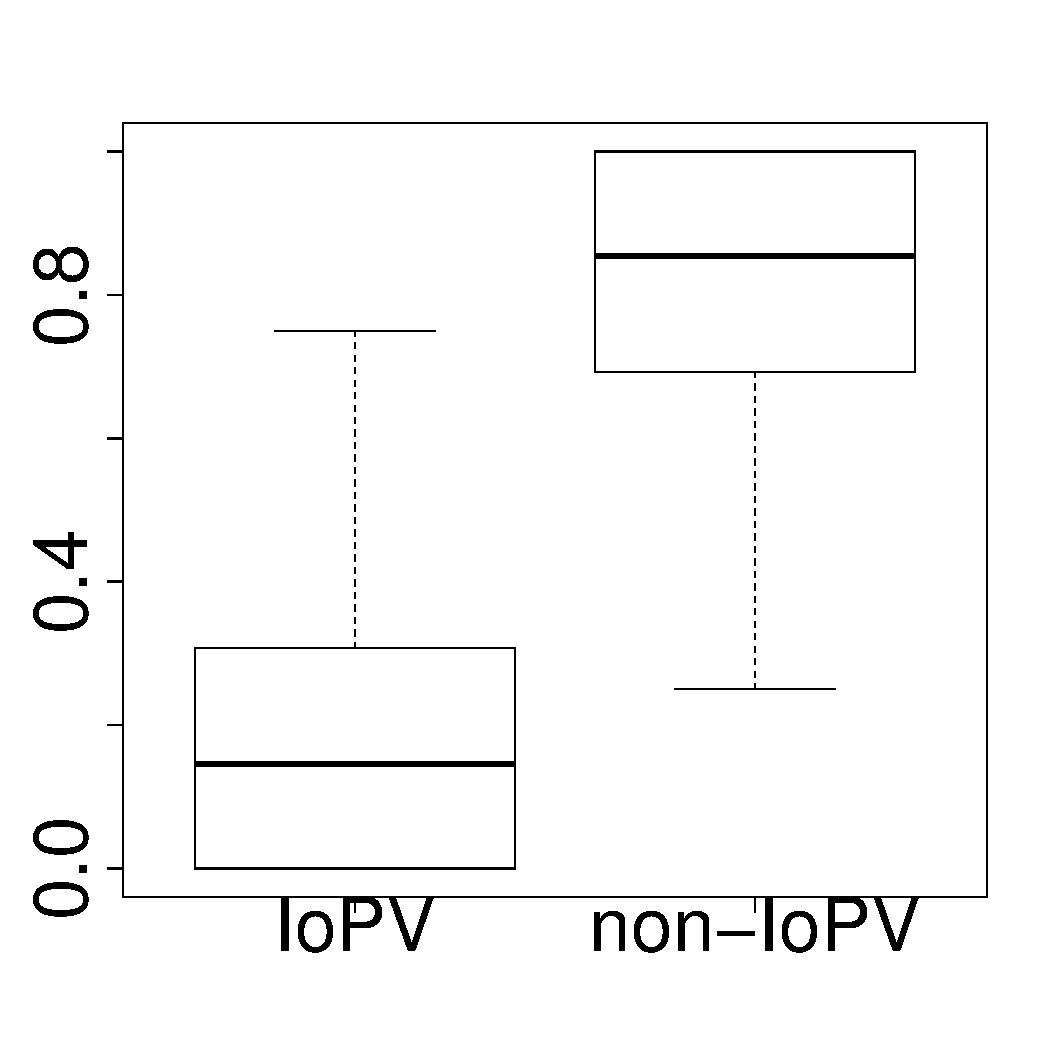
\includegraphics[width=\linewidth]{Figures/cpu-hadoop-boxplot.pdf}
                \caption{CPU}
        \end{subfigure}%
        \begin{subfigure}{0.19\textwidth}
                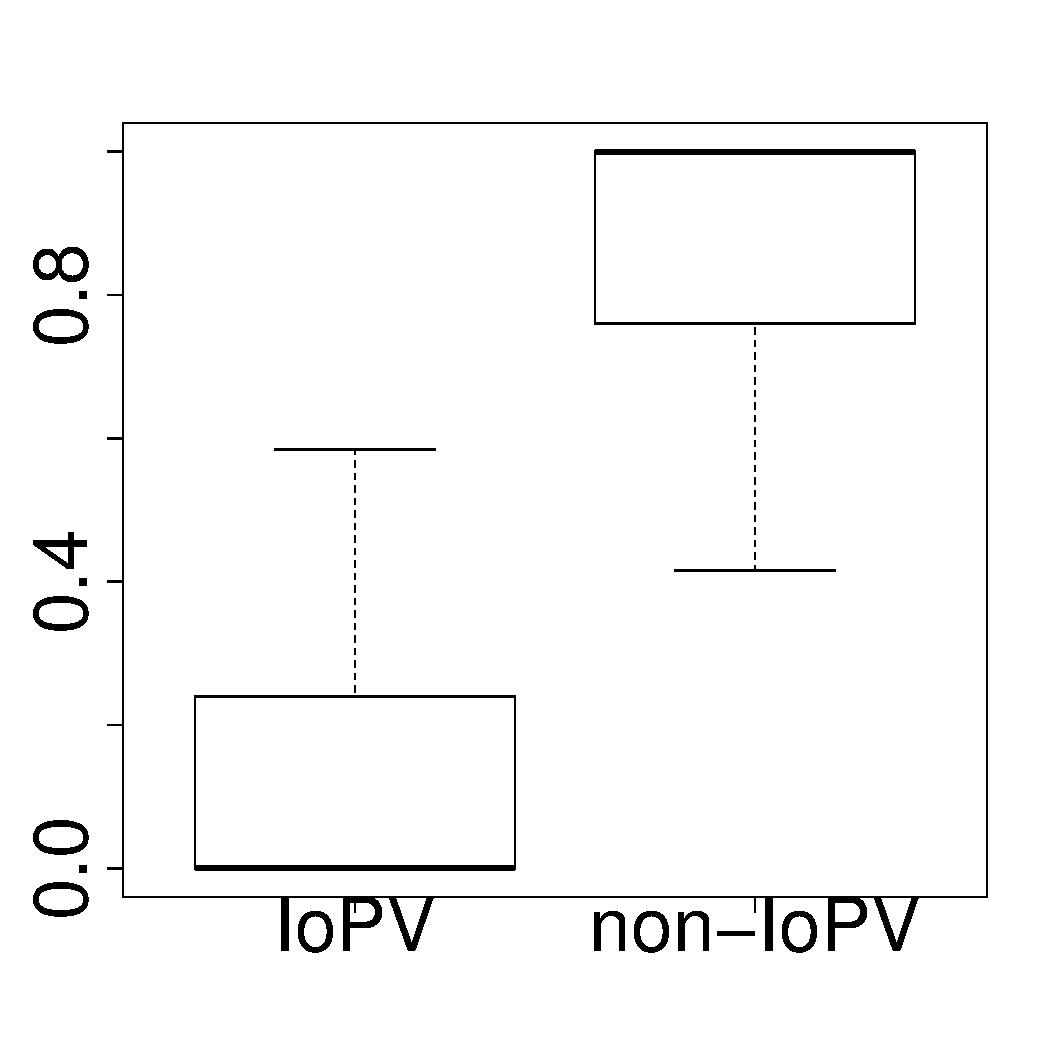
\includegraphics[width=\linewidth]{Figures/mem-hadoop-boxplot.pdf}
                \caption{Memory}
        \end{subfigure}%
        \begin{subfigure}{0.19\textwidth}
                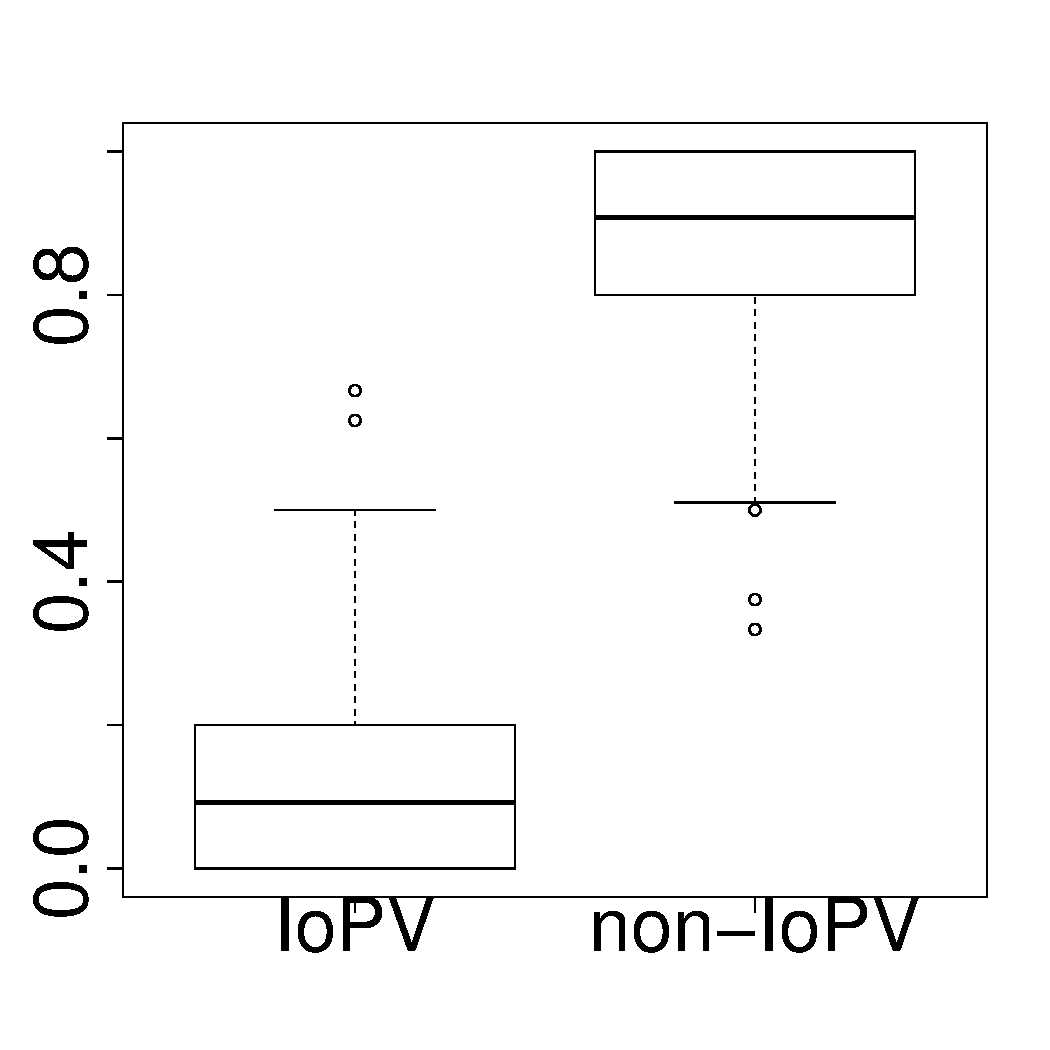
\includegraphics[width=\linewidth]{Figures/ioread-hadoop-boxplot.pdf}
                \caption{I/O read}
        \end{subfigure}
        \begin{subfigure}{0.19\textwidth}
                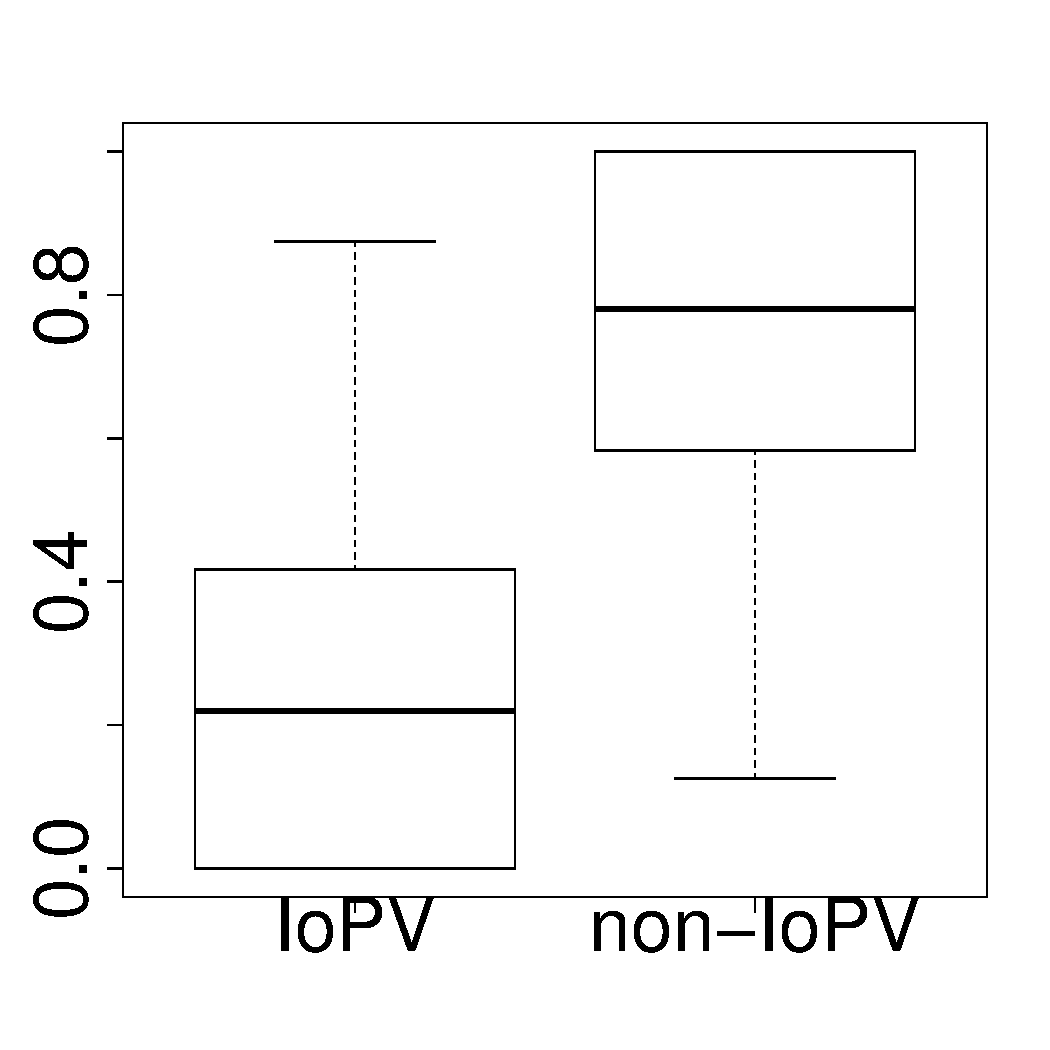
\includegraphics[width=\linewidth]{Figures/iowrite-hadoop-boxplot.pdf}
                \caption{I/O write}
        \end{subfigure}
        
	\caption{Percentage of \inconsistent for each commit of \emph{Hadoop}.}
	\label{fig:iopv_per_commit_hadoop}
% 	\vspace{-0.15cm}
\end{figure}

\begin{figure}[t]
	\centering
        \begin{subfigure}{0.19\textwidth}
                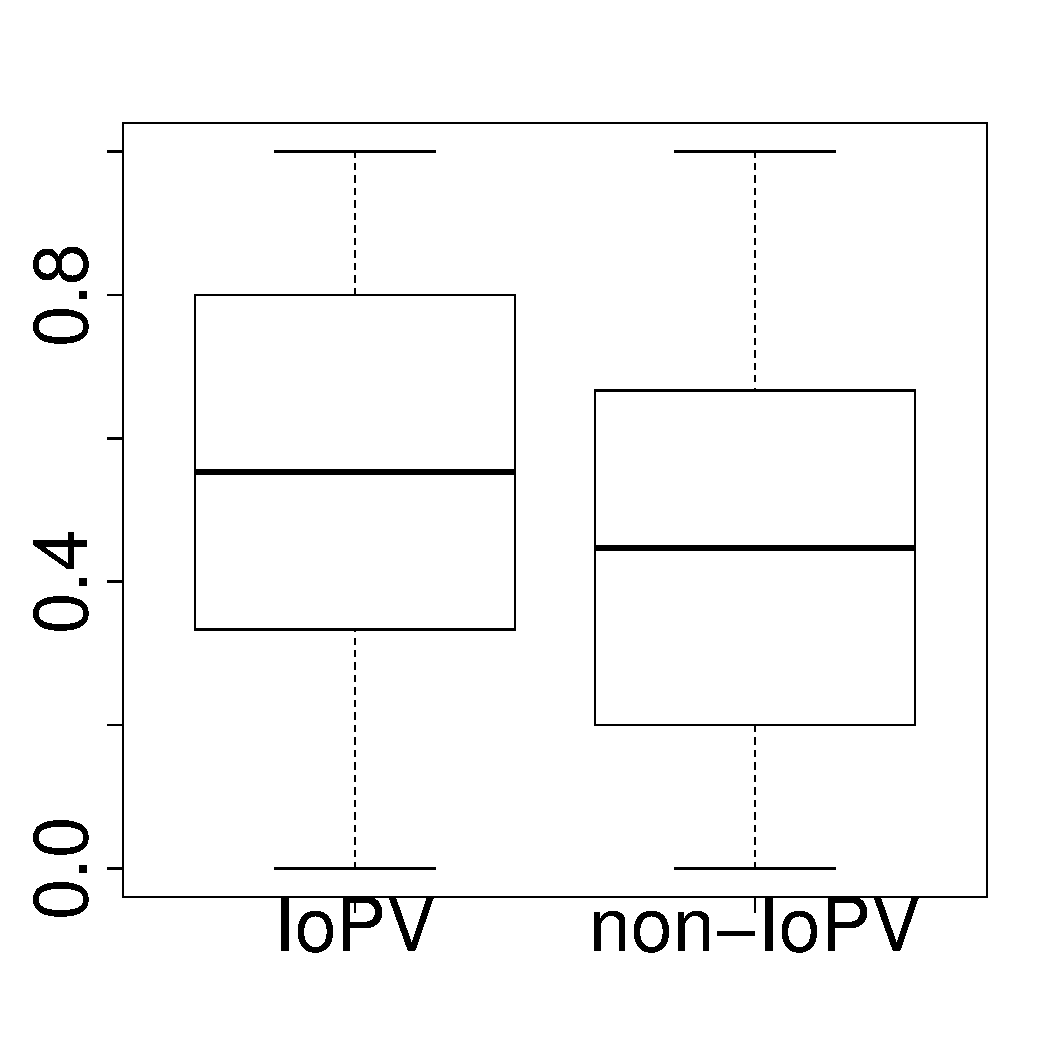
\includegraphics[width=\linewidth]{Figures/runtime-cassandra-boxplot.pdf}
                \caption{Res. time}
        \end{subfigure}%
        \begin{subfigure}{0.19\textwidth}
                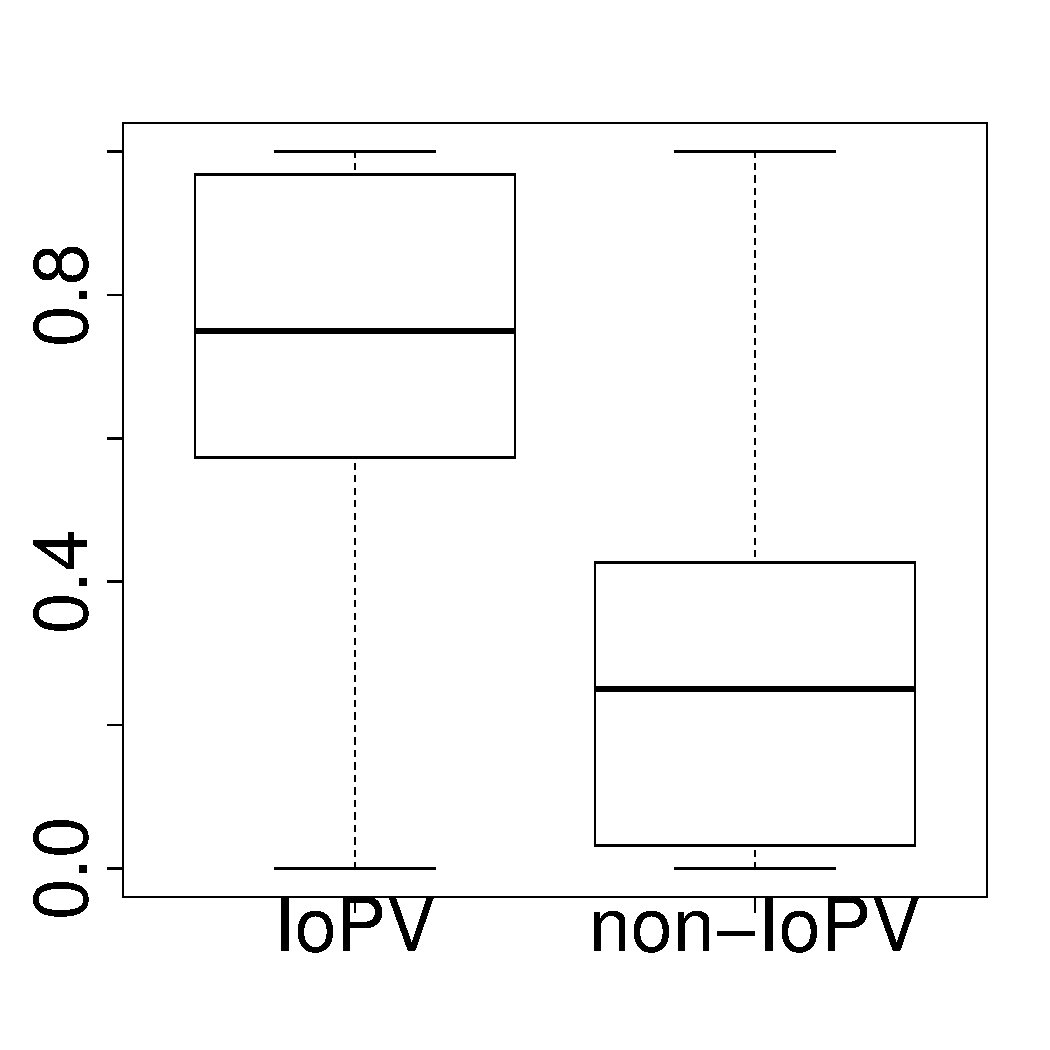
\includegraphics[width=\linewidth]{Figures/cpu-cassandra-boxplot.pdf}
                \caption{CPU}
        \end{subfigure}%
        \begin{subfigure}{0.19\textwidth}
                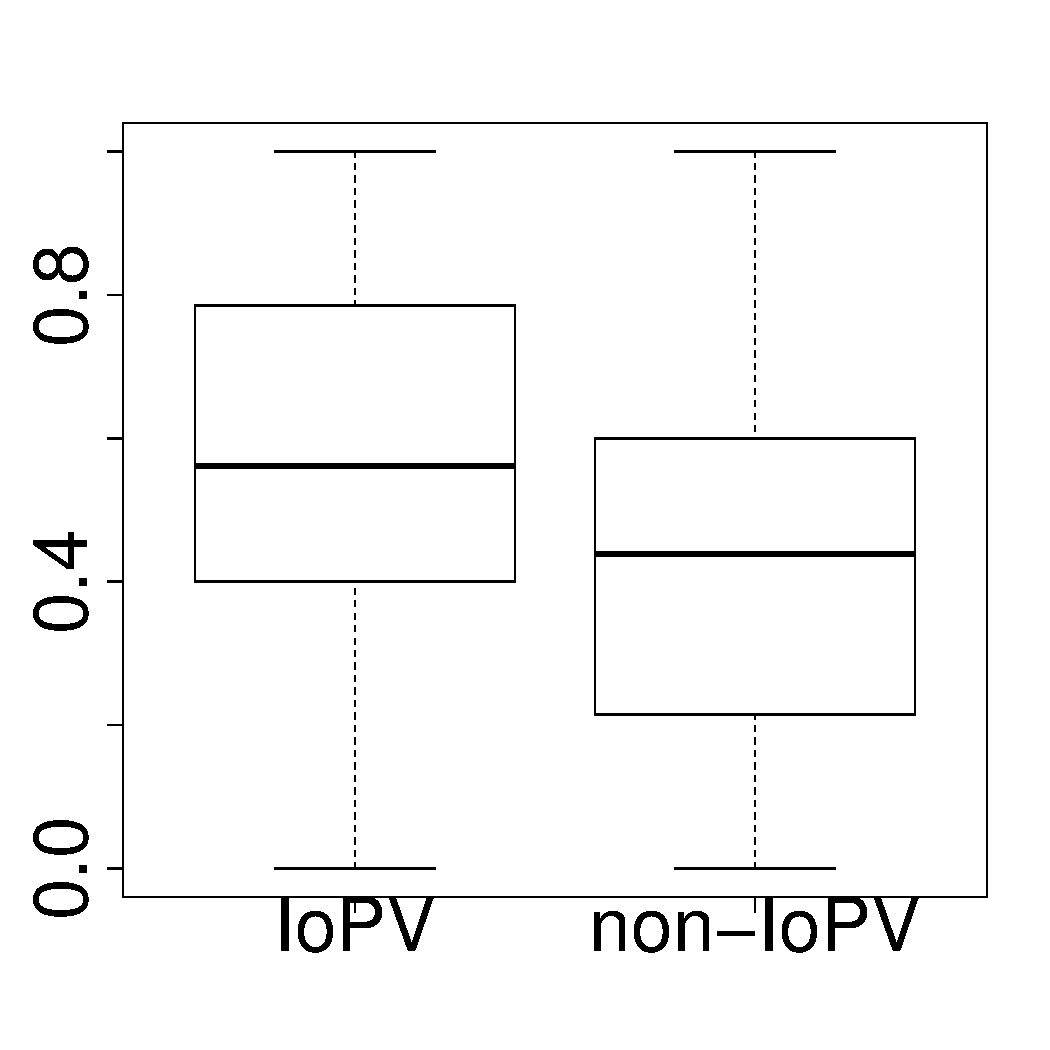
\includegraphics[width=\linewidth]{Figures/mem-cassandra-boxplot.pdf}
                \caption{Memory}
        \end{subfigure}%
        \begin{subfigure}{0.19\textwidth}
                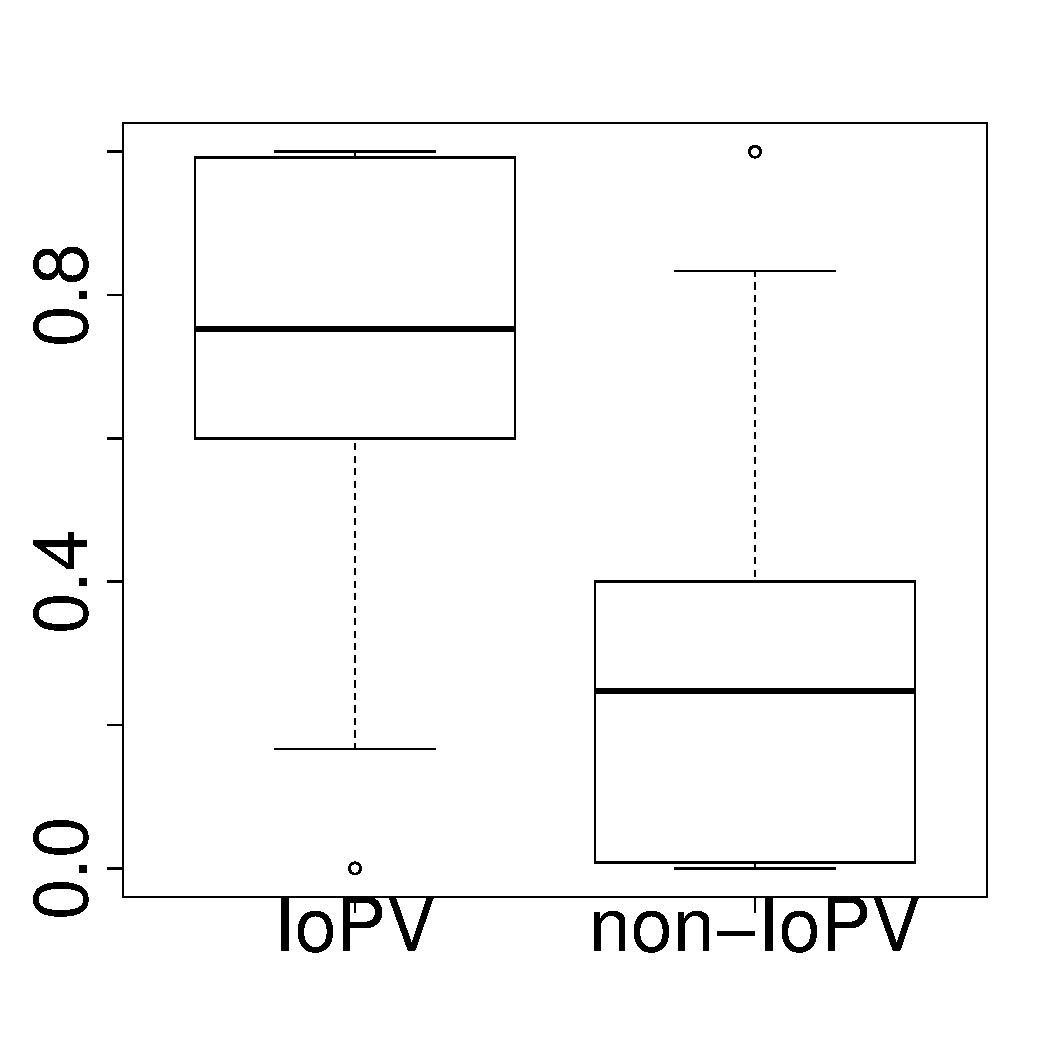
\includegraphics[width=\linewidth]{Figures/ioread-cassandra-boxplot.pdf}
                \caption{I/O read}
        \end{subfigure}
        \begin{subfigure}{0.19\textwidth}
                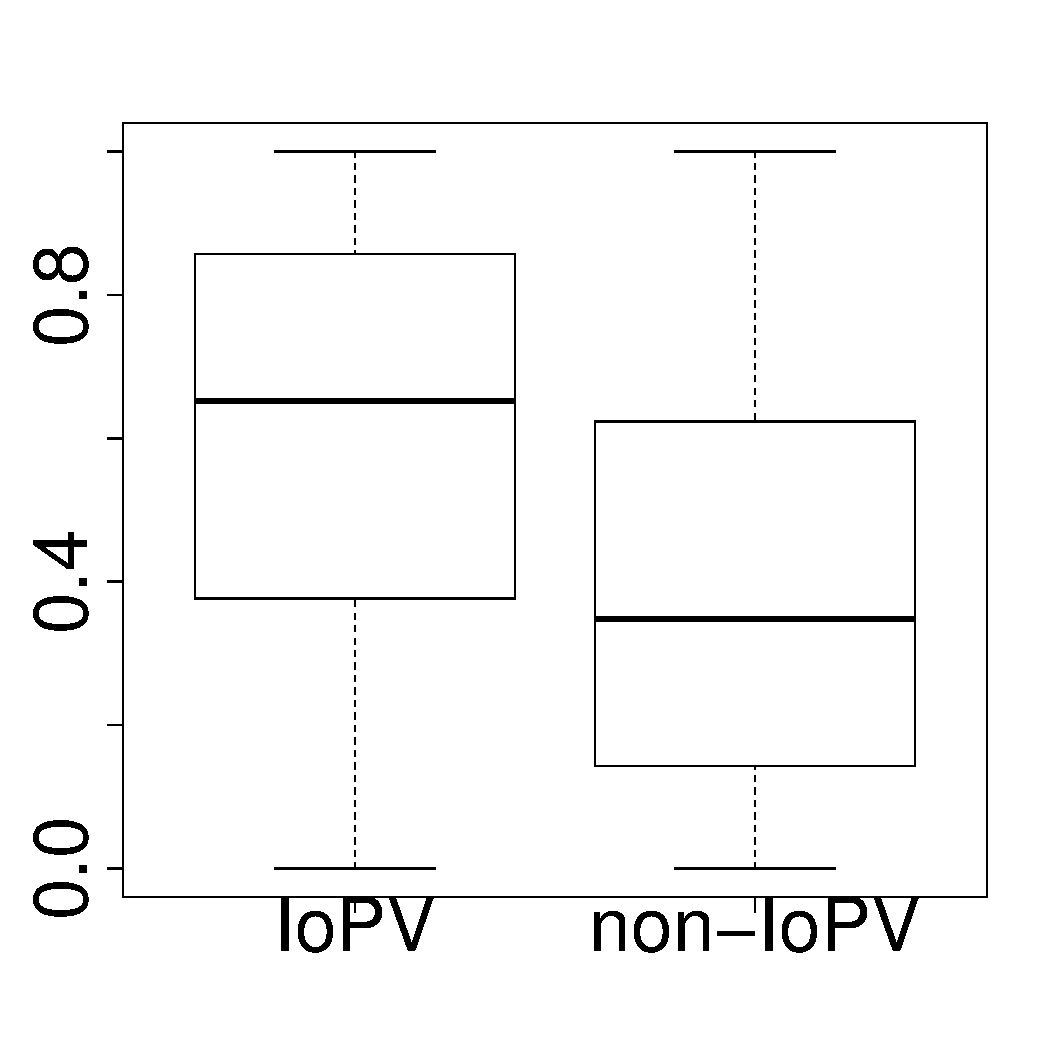
\includegraphics[width=\linewidth]{Figures/iowrite-cassandra-boxplot.pdf}
                \caption{I/O write}
        \end{subfigure}
        
	\caption{Percentage of \inconsistent for each commit of \emph{Cassandra}.}
	\label{fig:iopv_per_commit_cassandra}
% 	\vspace{-0.15cm}
\end{figure}


24\% and 54\% of the \instance in \emph{Hadoop} and \emph{Cassandra}, respectively, show a performance regression on at least one performance measure when the default configuration does not show any performance regression. %\noindent \textbf{The choice of \bram{default?} configuration option values may have a direct impact on the manifestations of performance regressions in a given code change compared to the previous state of the code base.} 
68\% and 89\% of our studied commits in \emph{Hadoop} and \emph{Cassandra} have at least one \instance that shows a performance regression under one non-default configuration while showing no regression under the default configuration, which indicates that having a hidden performance regression is common. For instance, we observe a performance regression in terms of response time on 42 and 1,023 out of 4,902 and 4,197 \emph{Hadoop} and \emph{Cassandra} \instance, respectively, when the default configuration does not show any regression, as shown in Table~\ref{tab:option_regression}. As shown in the same Table, the performance measure that suffers the most from the \inconsistent problem %\instance that show a performance regression when no regression is observed on the default configuration corresponds to 
are the I/O write and CPU measures. %, with 626 Hadoop and 1,446 Cassandra \instance cases, respectively. 
In addition, these are not minor regression differences, as 78\% of the regressions are large based on our effect size analysis. 

%The impact of different configurations on the manifestations of performance regression is shown in Table~\ref{tab:option_regression}. %We executed a total of 4,902 and 4,785 commit-test-option (\instance) cases in \emph{Hadoop} and \emph{Cassandra}, respectively. \instance means the same option with different option values in a specific test within a specific commit. For each \instance, we execute the impacted tests with default value and other option values (see subsection~\ref{evaluation}). We find that there exist a large number of options with performance regression. 

%For example, 70 and 1,567 out of a total of 4,902 \emph{Hadoop} \instance and 4,785 \emph{Cassandra} \instance % from , 70 and 1,567 
%have statistically significantly slower response time, respectively. 
%\bram{this means that out of the 2 non-default values at least one showed slowdown? or would a slowdown for both non-default values be counted twice?} \bram{also, what is the range of slowdown, e.g., X\% of cases had up to a Y-fold slowdown, while Z\% had a slowdown of more than W-fold}

14\% and 20\% of the \instance in \emph{Hadoop} and \emph{Cassandra} show a performance regression when the default configuration shows a performance improvement. Therefore, improving the performance of a system should consider different configurations. For example, 439 and 594 \emph{Hadoop} and \emph{Cassandra} \instance show a CPU performance regression when the default configuration shows an improvement, as shown in Table~\ref{tab:option_improvement_default}. This problem occurs for all of the studied performance measures. Similarly to our last finding, 58\% and 65\% of the commits in \emph{Hadoop} and \emph{Cassandra}, and a median of 10\% and 14\% of \instance per commit in \emph{Hadoop} and \emph{Cassandra} are impacted by such a problem.

Note that we also observe cases for which an option manifests a regression under the default value, but a non-regression or even an improvement under other values of the same option, as shown in Table~\ref{tab:option_regression_default}.% problem on the default value of an option 



%More importantly, we find that there also exist \instance cases with no regression or improvement compared to the previous revision of the code for the default option value, while there are performance regressions for other option values. For example, 42 and 1,093 \instance cases do not show any performance regression for the default value, but show performance regressions for the other values in terms of response time in \emph{Hadoop} and \emph{Cassandra}, respectively. 

%We also use four popular physical performance metrics \bram{shouldn't this have been mentioned in the approach? also, previous paragraphs seem to have used those metrics already, or what metric was used? seems to be response time}, i.e., CPU usage, Memory allocation, I/O read, and I/O write to measure performance regression. We find that we can detect more \instance cases with performance regression than are identified with response time. For example, 1,092 and 2,529 option cases have performance regression in different option values in \emph{Hadoop} and \emph{Cassandra}, respectively. \bram{again, what factors of slowdown/memory blow-up?}
%When examining the effect size of the detected performance regressions, we find that there exist more large performance regressions than medium performance regression. \bram{boxplot with this information?} Such results confirm the need for performance assurance related to configuration options in practice, since they may have a large impact on system performance.

\begin{table}[t]
\tabcolsep=0.04cm
\caption{Number of \instance with no regression under the default option value but with regression under other option values. Medium (large) means the effect size \emph{Cliff\textquotesingle s delta} of performance regression is medium (large).} %\heng{Briefly explain median and large to make the table self-explainable}} %\med{This Table should have (default with no regression vs non default with regression) and (default with improvement vs non default with regression) and (default with regression, non-default without regression or with improvement). I think the first two are there, but not the last one. }}
    \begin{tabular}{|c|c|c|r|c|r|c|r|c|r|c|r|}
    \hline
    %\multicolumn{12}{|c|}{Number of \instance with no regression in default   value but regression in other values}              \\ \hline
    \multirow{2}{*}{subject} & \multirow{2}{*}{\#CTO}    & \multicolumn{2}{c|}{Response time}    & \multicolumn{2}{c|}{CPU}               & \multicolumn{2}{c|}{Memory}           & \multicolumn{2}{c|}{I/O read}          & \multicolumn{2}{c|}{I/O write}         \\ \cline{3-12} 
            &          & large   & \multicolumn{1}{c|}{medium} & large    & \multicolumn{1}{c|}{medium} & large   & \multicolumn{1}{c|}{medium} & large    & \multicolumn{1}{c|}{medium} & large    & \multicolumn{1}{c|}{medium} \\ \hline
    Hadoop  & \multicolumn{1}{r|}{4,902} & \multicolumn{1}{r|}{24}  & 18         & \multicolumn{1}{r|}{517}  & 84         & \multicolumn{1}{r|}{208} & 214        & \multicolumn{1}{r|}{208}  & 214        & \multicolumn{1}{r|}{528}  & 98         \\ \hline
    Cassandra                & \multicolumn{1}{r|}{4,197} & \multicolumn{1}{r|}{600} & 423        & \multicolumn{1}{r|}{1,094} & 352        & \multicolumn{1}{r|}{788} & 404        & \multicolumn{1}{r|}{1,033} & 363        & \multicolumn{1}{r|}{921} & 326        \\ \hline
    \end{tabular}
\label{tab:option_regression}
\end{table}

\begin{table}[t]
\tabcolsep=0.04cm
\caption{Number of \instance with improvement under the default option value but with regression under other option values.}
    \begin{tabular}{|c|c|c|r|c|r|c|r|c|r|c|r|}
    \hline
    %\multicolumn{12}{|c|}{Number of \instance with improvement in default   value but regression in other values} \\ \hline
    \multirow{2}{*}{subject} & \multirow{2}{*}{\#CTO}    & \multicolumn{2}{c|}{Response time}    & \multicolumn{2}{c|}{CPU}       & \multicolumn{2}{c|}{Memory}    & \multicolumn{2}{c|}{I/O read}  & \multicolumn{2}{c|}{I/O write} \\ \cline{3-12} 
     &   & large   & \multicolumn{1}{c|}{medium} & large   & \multicolumn{1}{c|}{medium} & large   & \multicolumn{1}{c|}{medium} & large   & \multicolumn{1}{c|}{medium} & large   & \multicolumn{1}{c|}{medium} \\ \hline
    Hadoop  & \multicolumn{1}{r|}{4,902} & \multicolumn{1}{r|}{4}   & 3   & \multicolumn{1}{r|}{425} & 14  & \multicolumn{1}{r|}{102} & 36  & \multicolumn{1}{r|}{170} & 30  & \multicolumn{1}{r|}{426} & 46  \\ \hline
    Cassandra                & \multicolumn{1}{r|}{4,197} & \multicolumn{1}{r|}{122} & 53  & \multicolumn{1}{r|}{450} & 95 & \multicolumn{1}{r|}{220} & 52  & \multicolumn{1}{r|}{412} & 93 & \multicolumn{1}{r|}{327} & 74  \\ \hline
    \end{tabular}
\label{tab:option_improvement_default}
\end{table}

\begin{table}[t]
\tabcolsep=0.04cm
\caption{Number of \instance with regression under the default option value and  non-regression/improvement under other values.}
    \begin{tabular}{|c|c|c|r|c|r|c|r|c|r|c|r|}
    \hline
    %\multicolumn{12}{|c|}{Number of \instance with regression in default value and  non-regression/improvement in other values}             \\ \hline
    \multirow{2}{*}{subject} & \multirow{2}{*}{\#CTO}    & \multicolumn{2}{c|}{Response time}                     & \multicolumn{2}{c|}{CPU}     & \multicolumn{2}{c|}{Memory}  & \multicolumn{2}{c|}{I/O read}& \multicolumn{2}{c|}{I/O write}   \\ \cline{3-12} 
       & & large                    & \multicolumn{1}{c|}{medium} & large                    & \multicolumn{1}{c|}{medium} & large                    & \multicolumn{1}{c|}{medium} & large                    & \multicolumn{1}{c|}{medium} & large                    & \multicolumn{1}{c|}{medium} \\ \hline
    Hadoop                   & \multicolumn{1}{r|}{4,902} & \multicolumn{1}{r|}{17}  & 9 & \multicolumn{1}{r|}{431} & 60& \multicolumn{1}{r|}{128} & 200   & \multicolumn{1}{r|}{228} & 64& \multicolumn{1}{r|}{441} & 86\\ \hline
    Cassandra                & \multicolumn{1}{r|}{4,197} & \multicolumn{1}{r|}{236} & 222   & \multicolumn{1}{r|}{592} & 298   & \multicolumn{1}{r|}{314} & 229   & \multicolumn{1}{r|}{553} & 264   & \multicolumn{1}{r|}{439} & 229   \\ \hline
    \end{tabular}
\label{tab:option_regression_default}
\end{table}




\subsection*{\textbf{PQ2. \PQII}}

\subsubsection*{Motivation}

The goal of this preliminary question is to understand how difficult the manual prediction of \inconsistent (i.e., identification of \inconsistent without running the tests) is. For instance, the higher the number of options that manifest an \inconsistent in a large number of commits and tests, the more difficult the identification of \inconsistent is, as it indicates that an \inconsistent can occur in an unexpected way and any option can be responsible for such a problem. On the other hand, the lower the number of options that suffer from an \inconsistent, the easiest it is to test all of these \inconsistent responsible options. 

\subsubsection*{Approach}

%For instance, the higher the number of options that manifest an \inconsistent in a larger number of commits and tests, the more difficult the identification of \inconsistent is. That indicates that an \inconsistent can occur in an unexpected way and any option can be responsible for such a problem. On the other hand, the lower the number of options that suffer from an \inconsistent, the easiest it is to test all of these \inconsistent responsible options. 
%To understand how common a performance regression can be hidden by certain configuration, we further investigate whether a hidden performance regression occurs just under a handful set of configurations or under different configurations. In fact, a regression that is shown under a few number of configurations might be easy to fix, while a performance regression that is caused by different configurations can be more difficult to predict. %In addition, we would like to know whether the configuration options that may cause the different manifestations of performance regressions are consistent across commits of the subjects systems. In other words, there may exist a small set of configuration options that always cause the different manifestations of performance regressions. 
To investigate the difficulty of identifying an \inconsistent, we calculate the intersection of the $<$test, option, \inconsistent$>$ triplets between each pair of commits %for each commit, we collect all the configuration options that show an \inconsistent. Then, %For every two consecutive commits, 
%we compare each pair of commits % their two sets of configuration options 
using the Jaccard similarity defined as follows:
\begin{equation}
% \vspace{-0.2cm}
% J(C1,C2) = \frac{C1 \cap C2}{C1 \cup C2}
J(C1,C2) = \frac{|CTO_{C1} \cap CTO_{C2}|}{|CTO_{C1} \cup CTO_{C2}|}
\end{equation} 
where $C1$ and $C2$ refer to every pair of commits (both consecutive and non-consecutive commits). $|CTO_{C1} \cap CTO_{C2}|$ is the number of \instance that share the same $<$test, option, \inconsistent$>$ (i.e., the intersection). 
%cause performance regression in both commits $C1$ and $C2$.
$|CTO_{C1} \cup CTO_{C2}|$ is the total number of unique $<$test, option, \inconsistent$>$ in commits $C1$ and $C2$ (i.e., the union). %We then transform the Jaccard similarity to Jaccard distance using \emph{$1-J(C1,C2)$}. 
The Jaccard distance ranges %from 
between 0 %to 
and 1, where a value of 1 means that the pair of commits share the same $<$test, option, \inconsistent$>$, while 0 indicates that the pair of commits does not share any $<$test, option, \inconsistent$>$.

%configurations under which a performance regression or \med{improvement too? right?}improvement is observed have no overlapping while 0 means that the two sets of configurations %options 
%are identical. 

%\heng{We can downplay the manual analysis; 1) do not mentioning it in the approach; 2) only use the manual analysis results to explain why different commits do not share similar tests/options with \inconsistent } Finally, \med{No need for a manual analysis, we reached our goal from the quantitative analysis} \jinfu{Removed?} we manually examine the options that may show the different manifestations of performance regressions are consistent across different commits. \ian{TODO} 

\subsubsection*{Results}

\noindent \textbf{\inconsistent problems are hard to manually predict.} In particular, 81\% and 100\% of the \emph{Hadoop} and \emph{Cassandra} %\heng{need to make the font of the system names consistent throughout the paper} 
commits show at least one \instance with an \inconsistent. Similarly, all the options of \emph{Hadoop} and \emph{Cassandra} suffer at least once from a \inconsistent through the studied commits. Table~\ref{tab:dimemssion_regression} shows more details about how common are \inconsistent for the studied commits, tests, and options. 
In summary, our results indicate that the \inconsistent problem is not limited to a small set of commits, tests, or options, which makes it challenge to predict which \instance would have an \inconsistent.

Even if most of the commits show at least one \inconsistent, it is not easy to predict which test and option may suffer from the \inconsistent. 
%That is supported by our investigation on how different $<$test, option, \inconsistent$>$ intersects, whose results are shown in 
Figure~\ref{fig:across-commit-hadoop} and Figure~\ref{fig:across-commit-cassandra} show the pairwise Jaccard distance between the $<test, option, \inconsistent>$ triplets of the studied commits in the \emph{Hadoop} and \emph{Cassandra} systems, respectively.
The figures indicate that most of the commits do not share any $<$test, option, \inconsistent$>$ (i.e., with dark cells), especially for the \emph{Cassandra} system (i.e., more dark cells).
In other words, different commits are unlikely to have the same tests and options that can lead to \inconsistent problems. % to execute and when they do, the tests and options do not show similar \inconsistent results.
Therefore, it is difficult for developers to manually identify which tests and options that they need to run and configure to verify the existence of \inconsistent.
%For example, when two commits share a test and an option \emph{O} to test, one commit does not show any \inconsistent for \emph{O}, when the other commits shows an \inconsistent for the same option.  

\begin{figure}[t]
	\centering
        \begin{subfigure}{0.19\textwidth}
                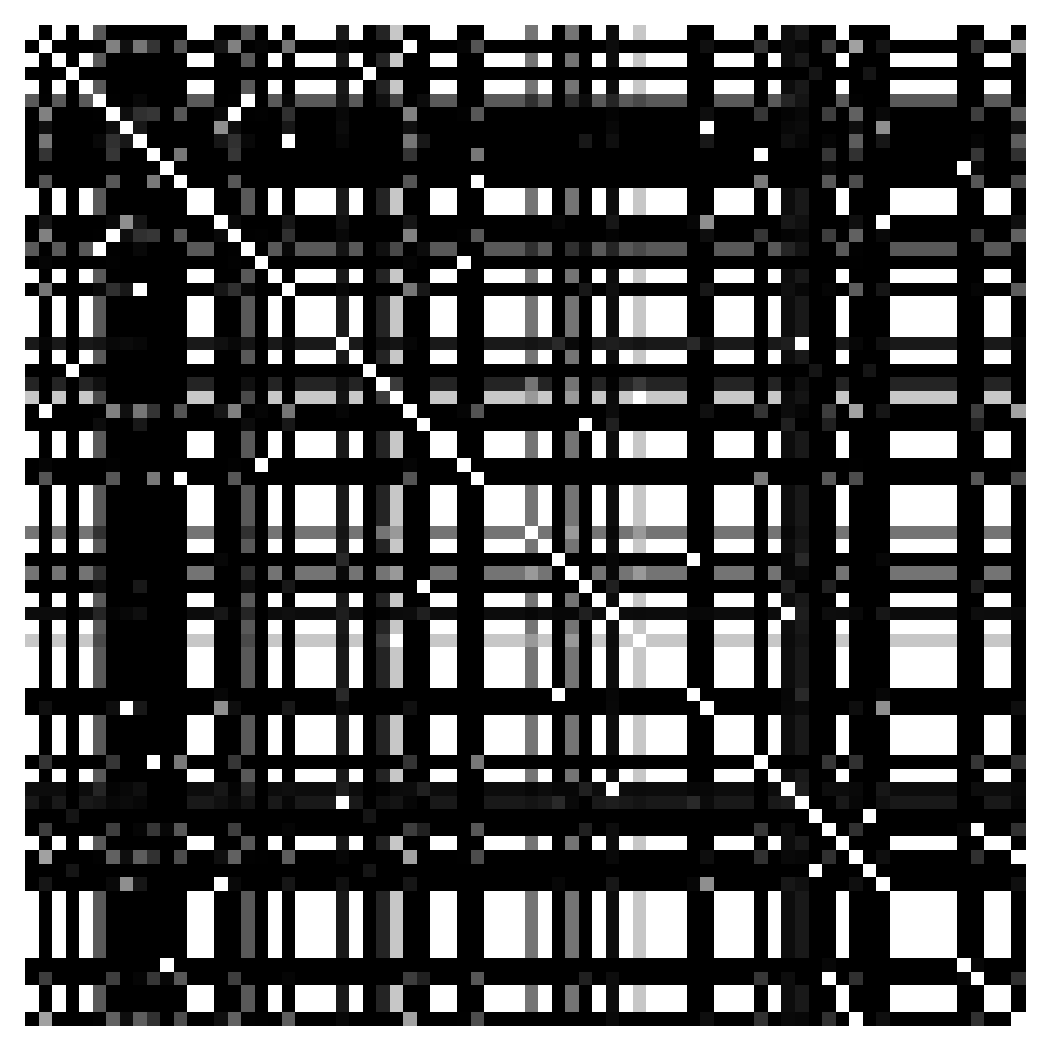
\includegraphics[width=\linewidth]{Figures/hadoop-runtime-commitX.pdf}
                \caption{Res. time}
        \end{subfigure}%
        \begin{subfigure}{0.19\textwidth}
                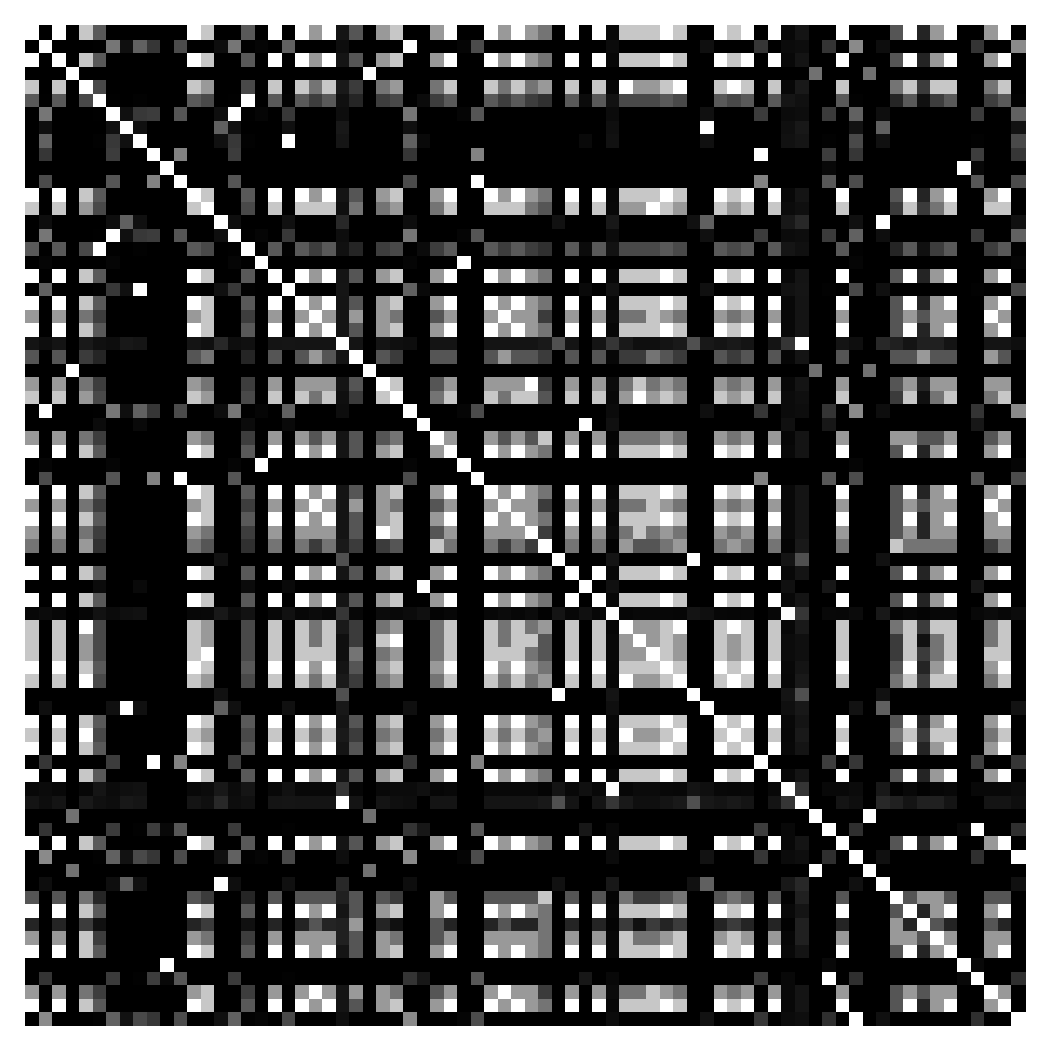
\includegraphics[width=\linewidth]{Figures/hadoop-cpu-commitX.pdf}
                \caption{CPU}
        \end{subfigure}%
        \begin{subfigure}{0.19\textwidth}
                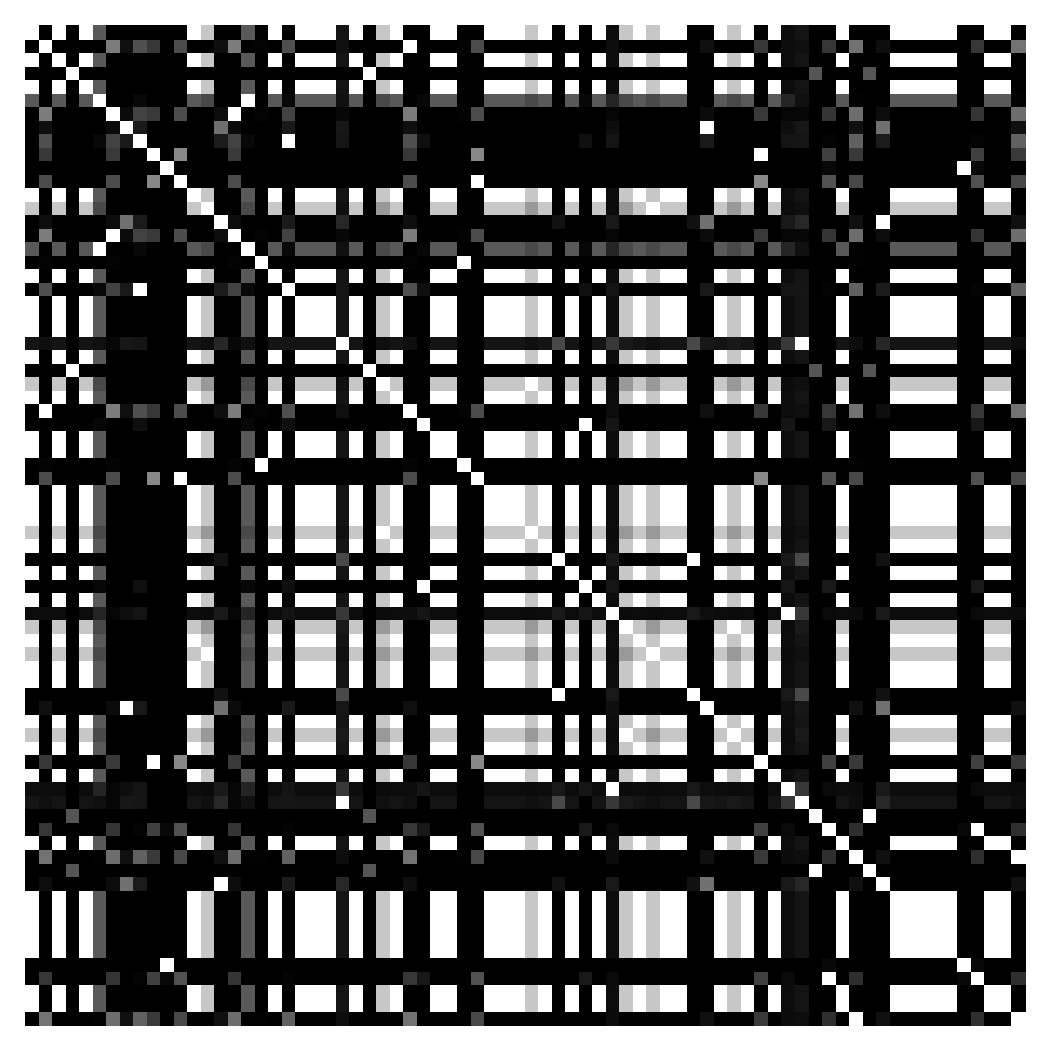
\includegraphics[width=\linewidth]{Figures/hadoop-mem-commitX.pdf}
                \caption{Memory}
        \end{subfigure}%
        \begin{subfigure}{0.19\textwidth}
                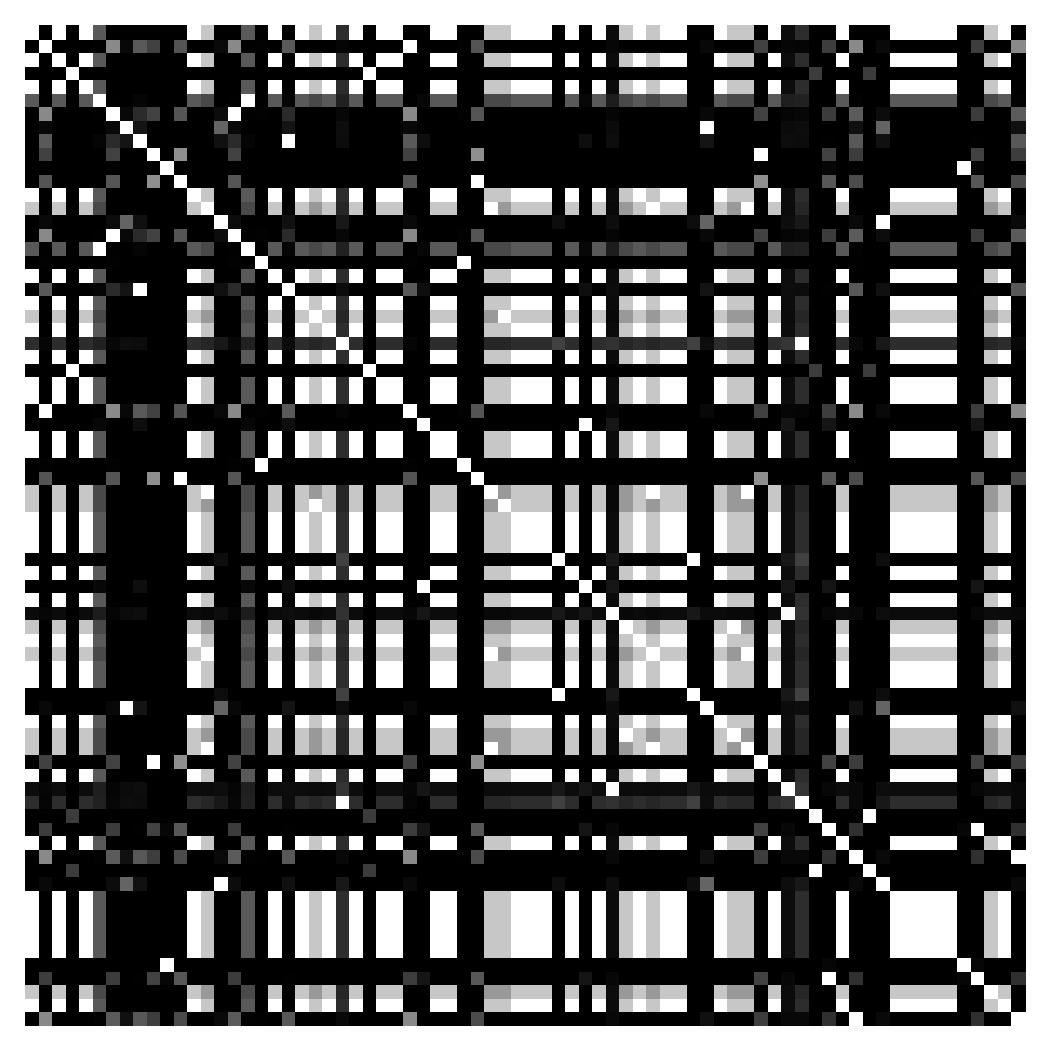
\includegraphics[width=\linewidth]{Figures/hadoop-ioread-commitX.pdf}
                \caption{I/O read}
        \end{subfigure}
        \begin{subfigure}{0.19\textwidth}
                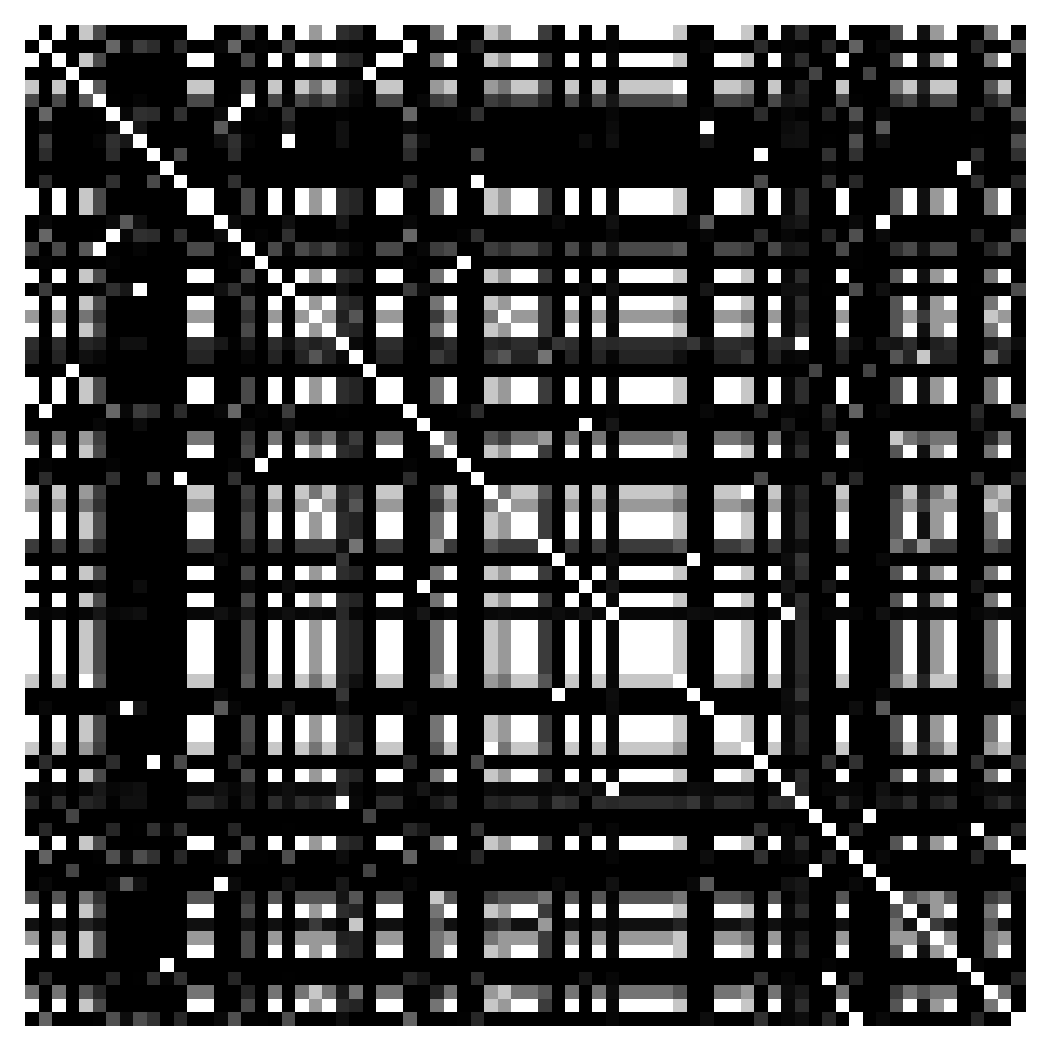
\includegraphics[width=\linewidth]{Figures/hadoop-iowrite-commitX.pdf}
                \caption{I/O write}
        \end{subfigure}
	\caption{Pairwise Jaccard distance between the $<test, option, \inconsistent>$ triplets of the studied commits of the \emph{Hadoop} system. The $x$-axis and $y$-axis show the studied commits, ordered chronologically from left to right on the $x$-axis and bottom to top on the $y$-axis. Each cell of the Figure refers to the Jaccard distance of any pair of commits: the darker the color is, the larger the distance is.}
	\label{fig:across-commit-hadoop}
% 	\vspace{-0.15cm}
\end{figure}

\begin{figure}[t]
	\centering
        \begin{subfigure}{0.19\textwidth}
                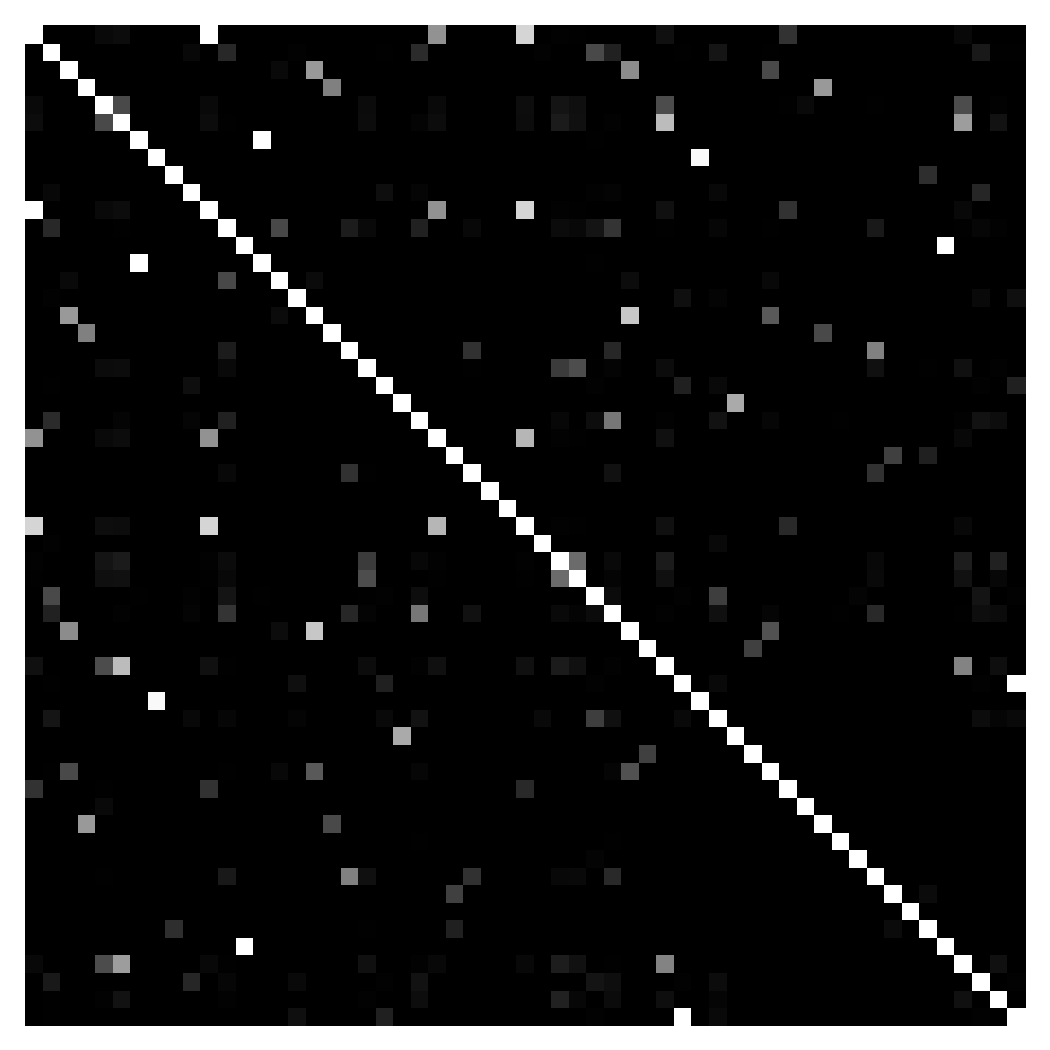
\includegraphics[width=\linewidth]{Figures/cassandra-runtime-commitX.pdf}
                \caption{Res. time}
        \end{subfigure}%
        \begin{subfigure}{0.19\textwidth}
                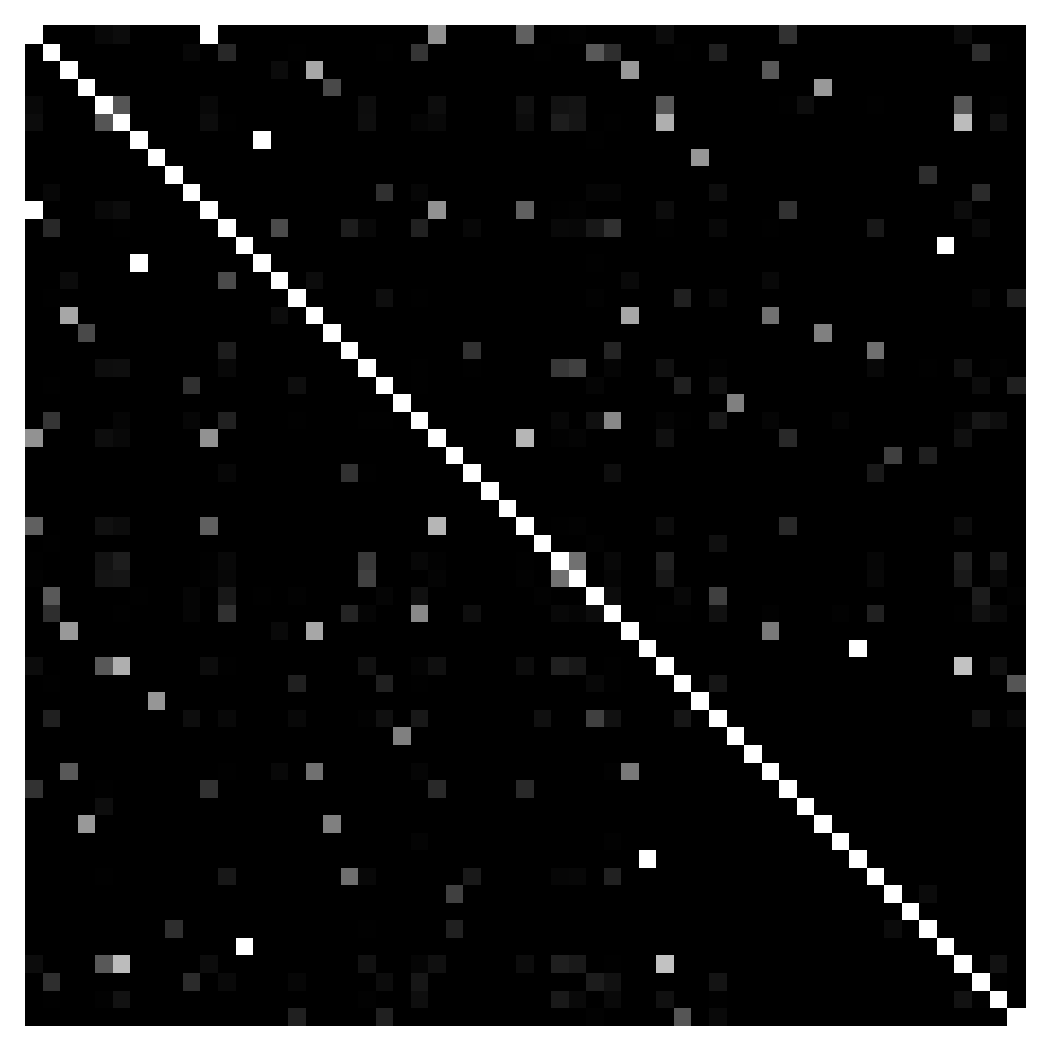
\includegraphics[width=\linewidth]{Figures/cassandra-cpu-commitX.pdf}
                \caption{CPU}
        \end{subfigure}%
        \begin{subfigure}{0.19\textwidth}
                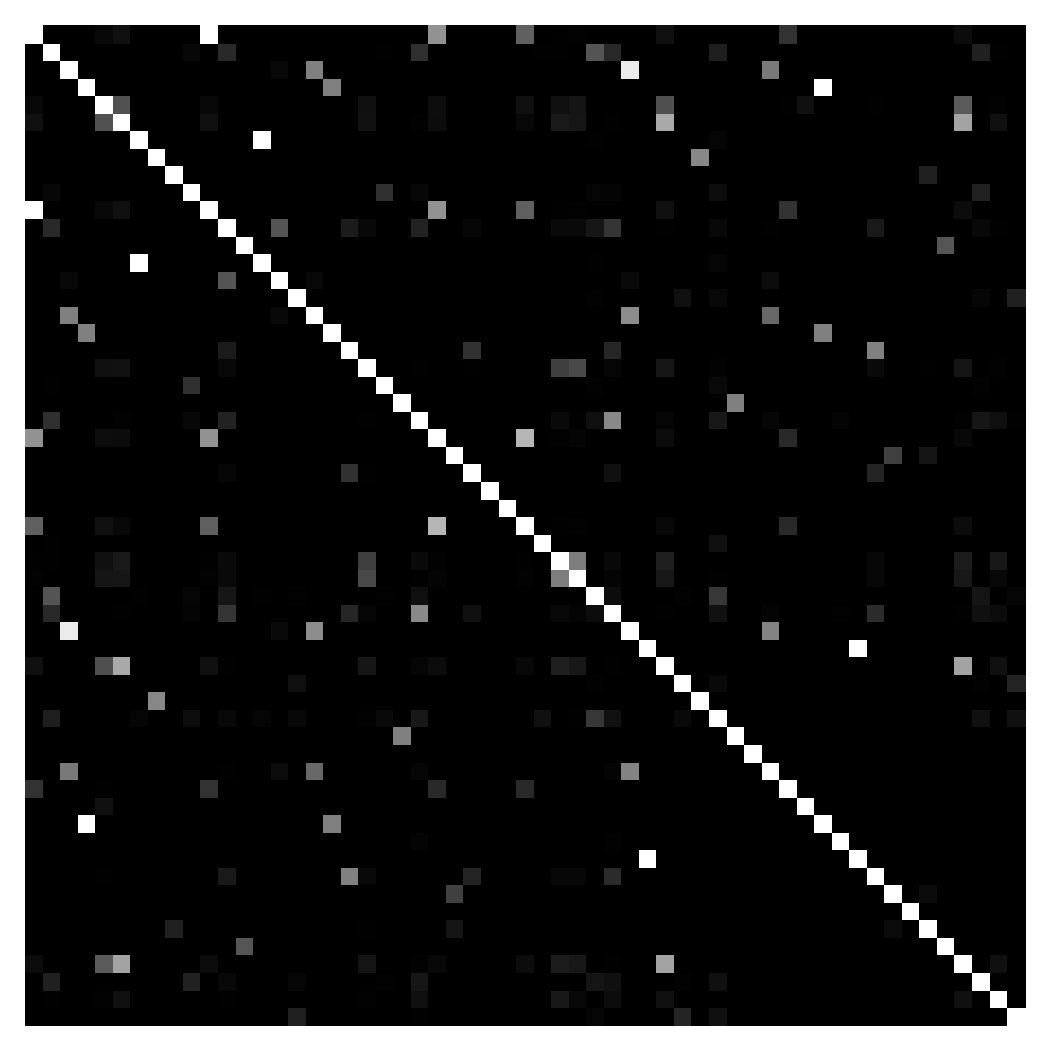
\includegraphics[width=\linewidth]{Figures/cassandra-mem-commitX.pdf}
                \caption{Memory}
        \end{subfigure}%
        \begin{subfigure}{0.19\textwidth}
                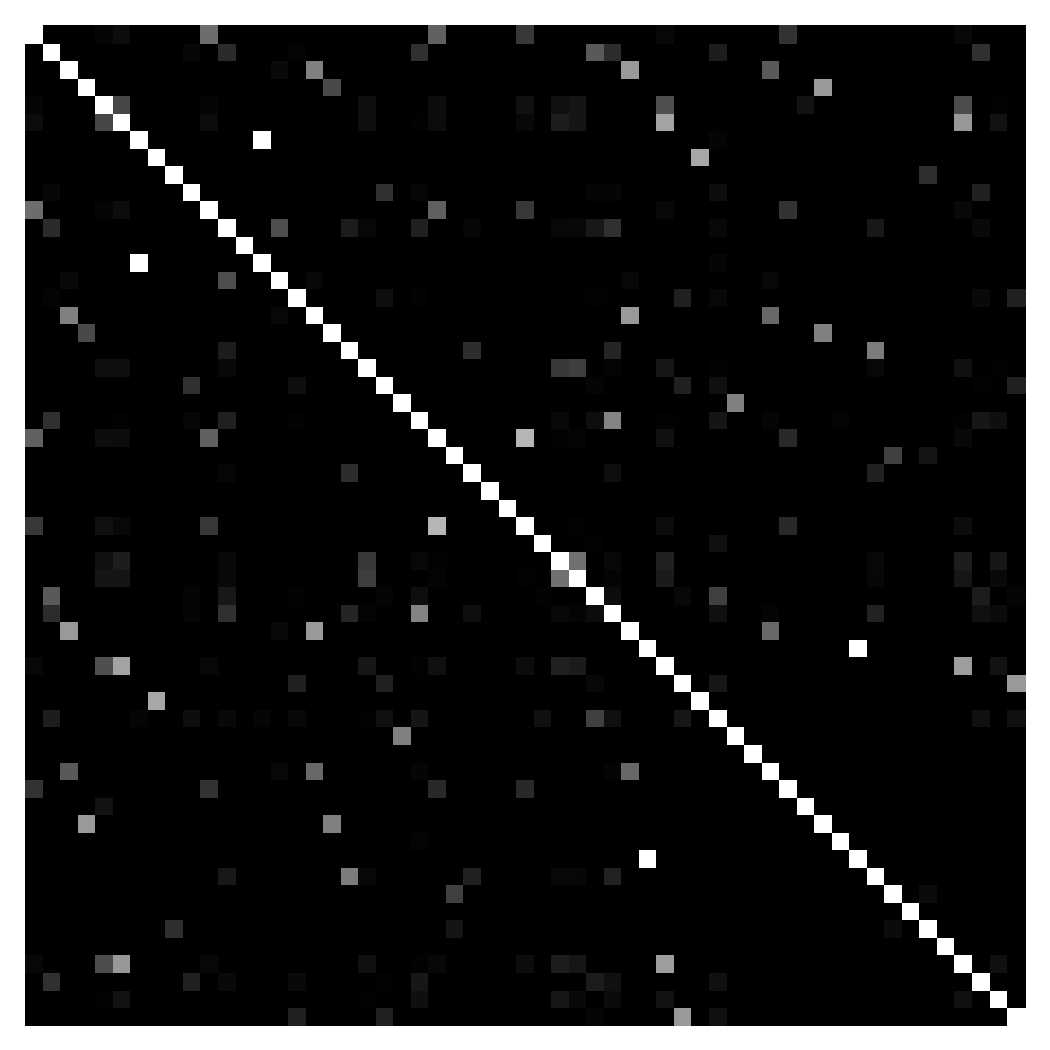
\includegraphics[width=\linewidth]{Figures/cassandra-ioread-commitX.pdf}
                \caption{I/O read}
        \end{subfigure}
        \begin{subfigure}{0.19\textwidth}
                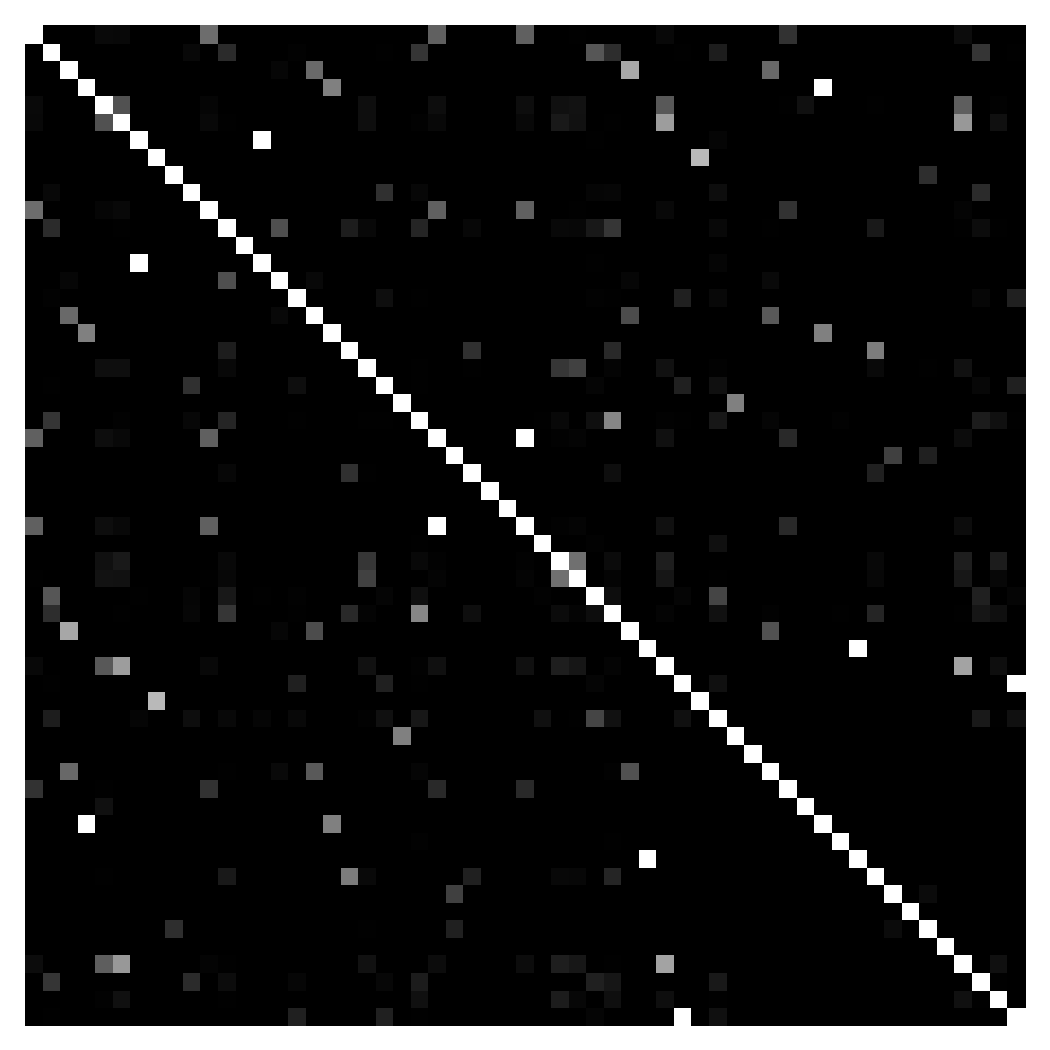
\includegraphics[width=\linewidth]{Figures/cassandra-iowrite-commitX.pdf}
                \caption{I/O write}
        \end{subfigure}
        
	\caption{Pairwise Jaccard distance between the $<test, option, \inconsistent>$ triplets of the studied commits of the \emph{Cassandra} system. The $x$-axis and $y$-axis show the studied commits, ordered chronologically from left to right on the $x$-axis and bottom to top on the $y$-axis. Each cell of the Figure refers to the Jaccard distance of any pair of commits: the darker the color is, the larger the distance is.}
	\label{fig:across-commit-cassandra}
% 	\vspace{-0.15cm}
\end{figure}

%we can note from Figure~\ref{fig:across-commit-hadoop}
%and Figure~\ref{fig:across-commit-cassandra} that most of the pairs of commits (cells) have a small distance (light blue color), with only a limited number of cases (dark horizontal/vertical lines) that have substantially different regressing options. 


%\med{-----------}

%\noindent \textbf{Performance regression manifested under a subset of the possible configurations is common.} We observe that 69\% (51 out of 74) of the \emph{Hadoop} and 93\% (53 out of 57) of the \emph{Cassandra} commits have at least one configuration with a performance regression manifested by one of our five studied performance measurement and under one of the executed tests. Similarly, we observe that 69 out of 74 of the \emph{Hadoop} and 202 out of 216 of the \emph{Cassandra} unit tests show at least one performance regression through the whole history and across different configurations. Table~\ref{tab:dimemssion_regression} shows more details about how common the performance is manifested for the studied commits, tests, configurations, and options' values. 


%Almost all the options 100\% (122 out of 122) and 80\% (43 out of 54) of \emph{Hadoop} and \emph{Cassandra} options) lead at least once (in one commit and test) to a performance regression, which indicate how difficult it is to identify configurations that hide a performance regression. That is in particular since the number of possible values leading to such issues is just \med{xyz\%} and \med{xyz\%} for \emph{Hadoop} and \emph{Cassandra}, respectively. The number of options manifesting a performance regression in our studied dataset is large for all the performance metrics, when the optoins' values leading to a regression issue is small as shown in Table~\ref{tab:dimemssion_regression}. 


%\noindent \textbf{The set of configuration options that may cause the different manifestations of performance regressions are not similar between commits.}
%The results of the number of commits, tests, and options with performance regressions are shown in Table~\ref{tab:dimemssion_regression}. \bram{where do these numbers occur in the table?} We note that 51 out of 74 (69\%) of the commits from \emph{Hadoop} and 53 out of 57 (93\%) of the commits from \emph{Cassandra} have at least one option with performance regression in any of the performance metrics. \bram{other observations in the table (a lot of numbers)?}

%When we measure the configuration options with performance regressions across commits of the subject systems, we find that the configuration options with performance regressions are not consistent across consecutive commits (see Figure~\ref{fig:across-commit-hadoop} and Figure~\ref{fig:across-commit-cassandra}). 
%\med{move to the figure caption}



%\med{I stopped here for this RQ, I would suggest to consider the value of options as well for figure 2. that can give better results. According to the previous paragraph, a lot of options have a regression somewhere but few values have a regression.}For instance, the configuration options with performance regressions are not consistent across consecutive commits, as shown in Figure~\ref{fig:across-commit-hadoop} and Figure~\ref{fig:across-commit-cassandra}. 


%\med{to review after discussing/addressing my previous comment}The two figures show that the set of configuration options that cause performance regressions mostly are the same in between commits. In particular, we can note from Figure~\ref{fig:across-commit-hadoop}
%and Figure~\ref{fig:across-commit-cassandra} that most of the pairs of commits (cells) have a small distance (light blue color), with only a limited number of cases (dark horizontal/vertical lines) that have substantially different regressing options. For example, in the case of response time for Hadoop, we notice two commits with entirely different sets of regressing options from the others, while the other options' regressing have substantial overlap. Response time for Cassandra has a higher number of medium to dark colored cells, but overall still features a majority of ligthly colored cells. In contrast, the plot for I/O write for Hadoop features a high density of dark lines, suggesting less consistent regressions.

%\med{That should move to the motivation of RQ2}These observations suggest that prediction models might obtain good performance in pinpointing regressing options for the cases with few dark lines. Especially Hadoop features substantial overlap between commits in terms of regression options. The next RQ builds and empirically validates such prediction models, aimed at warning developers of potential performance regressions for specific configuration options.%However, there exist a set of pairs of commits that have a large distance (dark blue color cell). For example, we find that \jinfu{give an example.}
 
%\noindent\med{I don't see the value for this manual analysis. What already exists (too much options, few values, and a lot of differences among the commits especially for Hadoop and Cassand I/O write) is good enough to motivate an automatic approach to predict the regressions.} \textbf{place holder for the manual examination} \bram{manually analyze interesting cases of response time Hadoop vs. Cassandra? i.e., few options responsible for large changes?} 

%To further understand the reason that configuration options cause different manifestations of performance regression between commit pairs, 
In order to understand why different commits show inconsistent $<test, option, \inconsistent>$ triplets, 
we manually analyze some commits that show the largest Jaccard distance from other commits (i.e., with dark horizontal/vertical lines in Figure~\ref{fig:across-commit-hadoop} and Figure~\ref{fig:across-commit-cassandra}). We consider the response time measure as an example in our manual analysis. 
In particular, there are two and six commits with large Jaccard distance ($>0.5$) to all other commits in \emph{Hadoop} and \emph{Cassandra}, respectively. 
%We find that many of the configuration options manifest performance regression in those commits. 
For \emph{Hadoop}, we find that most of the options cause \inconsistent in the test named \emph{TestKMS.java} in the \emph{Hadoop-common} sub-project. 
%Therefore, configuration practitioners can assign more focuses on the test \emph{TestKMS.java}. 
Then, we pick up one\footnote{\url{https://github.com/apache/hadoop/commit/b17d365f}} out of the two commits of \emph{Hadoop} to manually examine the configuration option and the commit changes. %\heng{Check if the following is right}
We find that the options that cause \inconsistent are usually related to connection time, such as the options \emph{dfs.ha.fencing.ssh.connect-timeout} and \emph{fs.s3a.connection.timeout}. By examining the code in the test \emph{TestKMS.java}, we find that \emph{TestKMS.java} loads the connection timeout configuration options. 
Thus, the commits that impact such connection time related options and the test may lead to \inconsistent problems while other commits may not lead to the same \inconsistent.
For \emph{Cassandra}, we select one commit \footnote{\url{https://github.com/apache/cassandra/commit/0fe82be8}} with the largest Jaccard distance to other commits. Our results show that two tests named \emph{EmbeddedCassandraServiceTest} and \emph{DebuggableScheduledThreadPoolExecutorTest} manifest the largest performance regression regarding options \emph{max\_hints\_file\_size\_in\_mb} and \emph{memtable\_heap\_space\_in\_mb}, respectively. By manually examining the commit changes covered by the tests, we find that there exist code changes in the method \emph{start} within the Java file \emph{EmbeddedCassandraService.java}\footnote{\url{https://github.com/apache/cassandra/blob/0fe82be83cceceb12172d63913388678253413bc/src/java/org/apache/cassandra/service/EmbeddedCassandraService.java#L53}}. Such a change adds function calls to initialize the options and leads to performance regressions. 
In summary, different commits may lead to different options and tests that exhibit \inconsistent problems.




\begin{table}[t]
    \centering
    \caption{Number of unique commits, tests, options with \inconsistent problems.} %\med{change regression by \inconsistent. In other words, drop this table and add a similar one for \inconsistent, as regression is just one case of \inconsistent which we discuss in just one bold statement to give an idea about how things are dangerous}}
    % \tabcolsep=0.1cm
    \begin{tabular}{|c|c|r|r|r|r|r|r|}
    \hline
    \multirow{2}{*}{}          & \multirow{2}{*}{} & \multicolumn{2}{c|}{Commit}      & \multicolumn{2}{c|}{Test}        & \multicolumn{2}{c|}{Option}      \\ \cline{3-8} 
         &                   & \multicolumn{1}{c|}{Total} & \multicolumn{1}{c|}{IoPV} & \multicolumn{1}{c|}{Total} & \multicolumn{1}{c|}{IoPV} & \multicolumn{1}{c|}{Total} & \multicolumn{1}{c|}{IoPV} \\ \hline
    \multirow{6}{*}{Hadoop}    & Res. time         & 74   & 27  & 74   & 13  & 122  & 74  \\ \cline{2-8} 
         & CPU               & 74   & 47  & 74   & 62  & 122  & 113 \\ \cline{2-8} 
         & Memory            & 74   & 38  & 74   & 59  & 122  & 113 \\ \cline{2-8} 
         & I/O read          & 74   & 45  & 74   & 53  & 122  & 108 \\ \cline{2-8} 
         & I/O write         & 74   & 47  & 74   & 57  & 122  & 117 \\ \cline{2-8} 
         & Any metric        & 74   & 60  & 74   & 67  & 122  & 117 \\ \hline
    \multirow{6}{*}{Cassandra} & Res. time         & 57   & 55  & 216  & 189 & 54   & 43  \\ \cline{2-8} 
         & CPU               & 57   & 55  & 216  & 204 & 54   & 49  \\ \cline{2-8} 
         & Memory            & 57   & 53  & 216  & 202 & 54   & 43  \\ \cline{2-8} 
         & I/O read          & 57   & 56  & 216  & 202 & 54   & 44  \\ \cline{2-8} 
         & I/O write         & 57   & 53  & 216  & 192 & 54   & 39  \\ \cline{2-8} 
         & Any metric        & 57   & 56  & 216  & 208 & 54   & 50  \\ \hline
    \end{tabular}
    \label{tab:dimemssion_regression}
\end{table}

\begin{comment}
\begin{table}[t]
  \centering
  \caption{Number of executed tests with performance regression \bram{following is confusing:} in different configuration options with different values}
  \tabcolsep=0.1cm
  \begin{tabular}{|c|c|c|r|c|r|c|r|c|r|c|r|}
    \hline
    \multirow{2}{*}{subject} & \multirow{2}{*}{\begin{tabular}[c]{@{}c@{}} \#Executed\\ tests\end{tabular}} & \multicolumn{2}{c|}{Response time}   & \multicolumn{2}{c|}{CPU}   & \multicolumn{2}{c|}{Memory}& \multicolumn{2}{c|}{I/O   read} & \multicolumn{2}{c|}{I/O   write}\\ \cline{3-12} 
     && large  & \multicolumn{1}{c|}{medium} & large  & \multicolumn{1}{c|}{medium} & large  & \multicolumn{1}{c|}{medium} & large  & \multicolumn{1}{c|}{medium} & large  & \multicolumn{1}{c|}{medium} \\ \hline
    Hadoop& \multicolumn{1}{r|}{13566}  & \multicolumn{1}{r|}{1708} & 128 & \multicolumn{1}{l|}{4180} & 342 & \multicolumn{1}{r|}{836}  & 562 & \multicolumn{1}{r|}{966}  & 178 & \multicolumn{1}{r|}{2626} & 292 \\ \hline
    Cassandra & \multicolumn{1}{r|}{30825}  & \multicolumn{1}{r|}{2353} & \multicolumn{1}{r|}{1852}   & \multicolumn{1}{r|}{6116} & \multicolumn{1}{r|}{2049}   & \multicolumn{1}{r|}{2729} & \multicolumn{1}{r|}{1749}   & \multicolumn{1}{r|}{5573} & \multicolumn{1}{r|}{2176}   & \multicolumn{1}{r|}{5595} & \multicolumn{1}{r|}{1829}   \\ \hline
    \end{tabular}
  \label{tab:perf_regression}
\end{table}
\end{comment}


% \begin{figure*}[tbh]
% 	\centering
% 		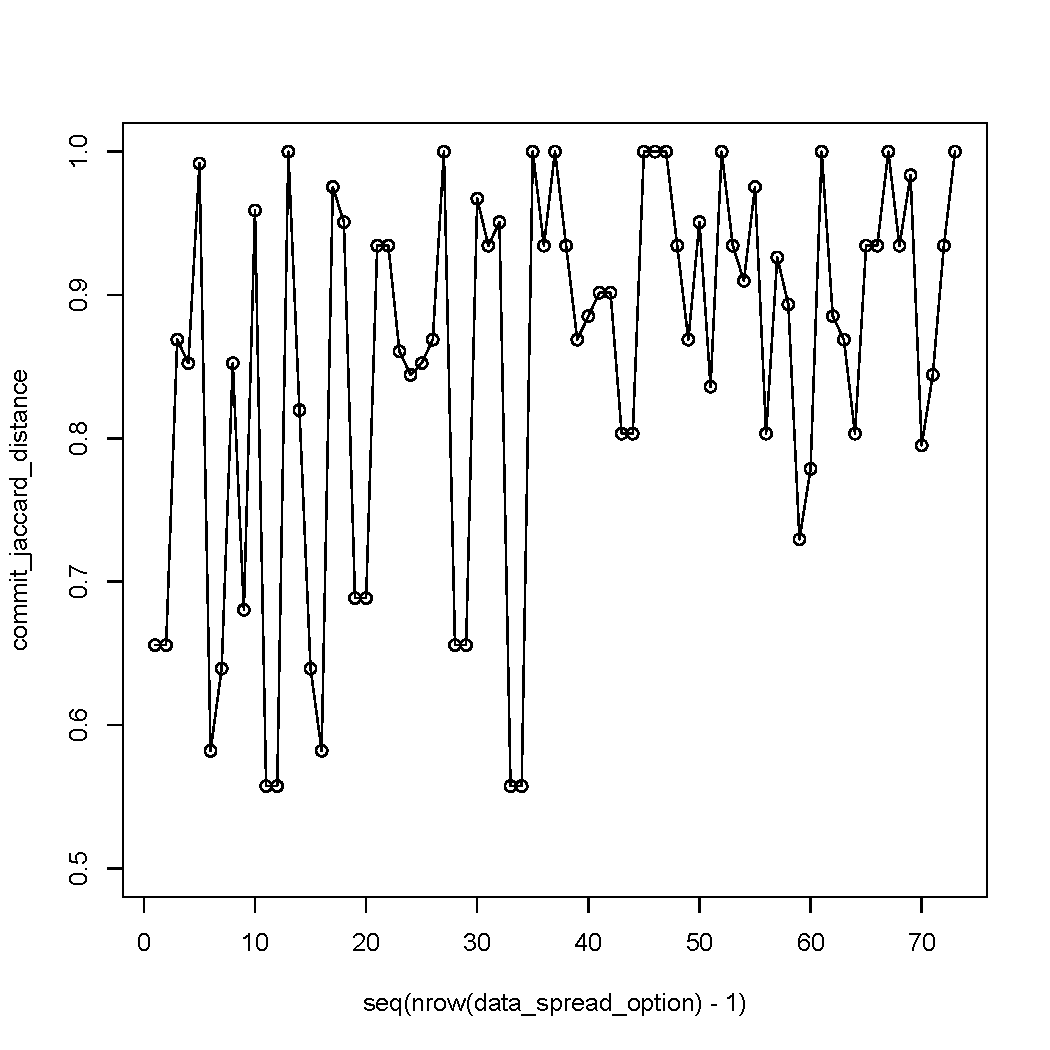
\includegraphics[width=.9\textwidth]{Figures/hadoop_restime.pdf}
% 	\caption{option change across commits.} 
% 	\label{fig:across-commit} 
% \end{figure*}



\begin{Summary}{Summary of Preliminary Study}{}
\inconsistent is a common problem and it is difficult to manually identify \inconsistent without exhaustively running the tests. Our results suggest the need for an approach that automatically identifies which \instance manifests an \inconsistent. 
\end{Summary}

\section{Predicting \inconsistent Problems} \label{sec:rq-results}

\subsection*{\textbf{RQ1. \RQII}}
\label{sec:rq2}

%\med{IMPORTANT NOTE: it's not ``caused'' by configuration, but just manifested under a subset of the existing configurations. The problem is not the configuration itself. }

%\med{we can add 2 RQs or enrich this RQ, by considering different dependent variables: if a config is different from the default config + when a config and a commit have a regression (which is the straightforward extension for Jinfu's prior work model) + what you already have, which is when we have a statistically significant variations of regression between different configurations}

%\med{todo: use option instead of parameter and make a clear distinction between configuration and option}
%\heng{Model is for per option, per commit, per test}\heng{TODO: update motivation and approach} 

%\heng{TODO: check and update results}

\subsubsection*{Motivation}

The goal of this research question is to evaluate different classification approaches on predicting for which \instance one has to check multiple option's values. %whether a commit, test, and configuration (i.e., \instance) will spot a performance regression. 
In our preliminary study, we observe that the \inconsistent is common and hard to manually predict, %is not equally manifested throughout all the configurations. %For instance, even if the default configuration does not show any performance regression, other configurations can badly suffer from a performance regression. %different settings of the configuration options significantly impact the results of performance regression detection. 
which indicates that developers need to test different values for each option. However, as there are typically a large number of configuration options (e.g., \emph{Hadoop} version 2.7.3 has 355 configuration options) with different possible values, exhaustively experimenting with all different options for each test in performance testing is time- and resource-consuming. In this RQ, we aim to reduce the effort of conducting configuration-aware performance testing by predicting the need for testing with different values for a given configuration option when a code change is made (i.e., for a \instance). Specifically, our approach predicts whether a \instance manifests an \inconsistent, such that developers can make an informed decision on whether they should consider different values for that option in their performance testing.

\subsubsection*{Approach}

In this RQ, we build ML models to predict whether a \instance manifests an \inconsistent. % detection after a code change is committed by developers 
%(i.e., the need to adjusting the configuration value of an \instance). 
Below, we describe the detailed steps involved in our modeling process.

\noindent\textbf{Step 1. Data preparation.}

\textit{Step 1.1. Defining the target variable.} Our target variable is a binary variable that indicates whether an \instance manifests an \inconsistent, which we obtained following the approach discussed in Section~\ref{sec:datacollection}. In particular, after collecting performance measurements, we calculated the performance variation for each option, and discretize each \instance into \inconsistent or non-\inconsistent following the discretization approach of Section~\ref{sec:statisticalAnalysis}.
%For each \instance, we use the maximum difference between the performance regression detection results with different values of a configuration option as the target variable.
%First, for each \instance, %commit, each test, and each configuration option, 
%we run performance testing using all different values of the option (repeated 30 times) and record the maximum difference between the performance regression detection results (i.e., the Cliff's delta effect size) using the default option value and other option values.


\begin{table}[t]
\tabcolsep=0.05cm
\scriptsize
\caption{Overview of our selected metrics.%\heng{the code tokens also include tokens from the test file right?}
}
\begin{tabular}{|l|l|l|}
\hline
Dimension & Metric           & Rationale \\ \hline
\multirow{8}{*}{\begin{tabular}[c]{@{}l@{}}Code \\      change\end{tabular}}    & \begin{tabular}[c]{@{}l@{}}Number   of modified\\      subsystems\end{tabular}   & \begin{tabular}[c]{@{}l@{}}The   more subsystems are changed, the higher risk\\      the change may be~\cite{mockus2000predicting}.\end{tabular}\\ \cline{2-3} 
  & \begin{tabular}[c]{@{}l@{}}Number of modified\\      directories\end{tabular}    & \begin{tabular}[c]{@{}l@{}}Changing   more directories may more likely introduce\\      performance regressions~\cite{mockus2000predicting}.\end{tabular}     \\ \cline{2-3} 
  & \begin{tabular}[c]{@{}l@{}}Number of modified\\      files\end{tabular}          & \begin{tabular}[c]{@{}l@{}}Changing   many source files are more likely to cause\\      performance regressions~\cite{Nagappan:2006:MMP}.\end{tabular}         \\ \cline{2-3} 
  & \begin{tabular}[c]{@{}l@{}}Distribution of modified\\      code across files\end{tabular}      & \begin{tabular}[c]{@{}l@{}}Scattered   changes are more possible to introduce\\      performance regressions~\cite{Hassan:2009:PFU}.\end{tabular}\\ \cline{2-3} 
  & \begin{tabular}[c]{@{}l@{}}Number of modified\\      methods\end{tabular}        & \begin{tabular}[c]{@{}l@{}}Changes   altering many methods are more likely \\      introduce performance regressions~\cite{Zimmermann:2007:PDE}.\end{tabular}  \\ \cline{2-3} 
  & \begin{tabular}[c]{@{}l@{}}Number of lines SOC\\ in tests\end{tabular} & \begin{tabular}[c]{@{}l@{}}Program   with more lines is more likely to \\      suffer from performance regressions~\cite{Koru2009tse}.\end{tabular}            \\ \cline{2-3} 
  & Lines of code added      & \begin{tabular}[c]{@{}l@{}}The   more lines of code added, the higher risk that the\\      program will suffer from performance   regressions~\cite{Nagappan:2005:URC,Zimmermann:2007:PDE}.\end{tabular} \\ \cline{2-3} 
  & Lines of code deleted    & \begin{tabular}[c]{@{}l@{}}The   more lines of code deleted, the higher risk of \\      performance regression is   introduced~\cite{Nagappan:2005:URC,Zimmermann:2007:PDE}.\end{tabular} \\ \hline
\multirow{4}{*}{\begin{tabular}[c]{@{}l@{}}Code \\      structure\end{tabular}} & \begin{tabular}[c]{@{}l@{}}Number of methods in\\      impacted test\end{tabular}& \begin{tabular}[c]{@{}l@{}}Program with   large number of methods is more\\      likely to suffer from performance regressions.\end{tabular}     \\ \cline{2-3} 
  & \begin{tabular}[c]{@{}l@{}}McCabe Cyclomatic\\      complexity\end{tabular}      & \begin{tabular}[c]{@{}l@{}}Program   with higher complexity is more likely to suffer\\      from performance regressions~\cite{Hassan:2009:PFU}.\end{tabular}  \\ \cline{2-3} 
  & \begin{tabular}[c]{@{}l@{}}Number of called\\      subprograms\end{tabular}      & \begin{tabular}[c]{@{}l@{}}Large   called subprograms will amplify the regression if \\      there exists performance regressions in the called   program~\cite{Nagappan:2006:MMP}.\end{tabular}         \\ \cline{2-3} 
  & \begin{tabular}[c]{@{}l@{}}Number of calling\\      subprograms\end{tabular}     & \begin{tabular}[c]{@{}l@{}}Large   calling subprograms will amplify the regressions if \\      there exists performance regressions in the called   program~\cite{Nagappan:2006:MMP}.\end{tabular}        \\ \hline
Code token& \begin{tabular}[c]{@{}l@{}}Code   tokens of the\\      changed source code\end{tabular}        & \begin{tabular}[c]{@{}l@{}}Some   code tokens may be more related to performance \\      than other tokens.\end{tabular}          \\ \hline
\begin{tabular}[c]{@{}l@{}}Configuration\\       option\end{tabular}            & \begin{tabular}[c]{@{}l@{}}Split   configuration\\      option names\end{tabular}            & \begin{tabular}[c]{@{}l@{}}The name components of a configuration option may be \\      related to a specific performance metric.\end{tabular}             \\ \hline
\end{tabular}
\label{tab:metrics}
\end{table}

\textit{Step 1.2. Selecting the features.}
We consider four dimensions of software metrics that are related to the likelihood of a configuration option impacting the performance testing of a code commit for each test (i.e., of an \instance). Table~\ref{tab:metrics} lists the detailed metrics used in our models. %\med{the hypothesis that link the four dimensions to the configuration performance regression doesn't make sense. I would suggest to say that ``
We already found in our prior work~\cite{jinfu_tse2020} that code structure, and code change dimensions are important for predicting performance regressions, but there we did not consider the impact of different configurations on the manifestation of performance regressions. Therefore, we use the prior dimensions as well as an additional dimension about the configuration options.

%\med{To reomve the following itemize about the dimensions:}
%\begin{itemize}
    %\item \heng{todo later: motivate the choice of metrics from RQ1 findings and Jinfu's prior performance regression model}
    \textbf{Code change metrics}. This dimension contains metrics that capture the code changes in a commit (e.g., the number of changed lines of code). Some code changes (e.g., big code changes) might be more likely to impact how different values of a configuration option make a difference in performance testing.
    
    \textbf{Code structure metrics}. This dimension contains metrics that describe the static structure of the source code files (e.g., cyclomatic complexity). %\med{not clear why? how a code change is related to a configuration? \jinfu{We have option-test mapping.}}
    Our intuition is that changing certain code (e.g., complex code) is more likely to alter the performance impact of a configuration option.
    
    \textbf{Code token metrics}. This dimension considers the code tokens of the methods that are changed in the commit and the test file.%\heng{can we separate the tokens from the source code and the test files into two dimensions?}. 
    Some code tokens (e.g., ``speed'') may be more related to performance than other tokens. We use the \emph{lscp}\footnote{Lscp is a lightweight source code preprocesser that can be used to isolate and manipulate the linguistic data (i.e., identifier names, comments, and string literals) from the source code: \url{https://github.com/doofuslarge/lscp}} tool to extract the code tokens from the source code. 
    
    \textbf{Configuration option metrics}. This dimension considers the characteristics of the configuration option, in particular the tokens in the configuration option names. We assume that some options (e.g., system resource-related options) are more likely to impact the performance regressions detection results of a commit.
%\end{itemize}


\textit{Step 1.3. Pre-processing the features.}
The code token metrics include thousands of unique code tokens. Thus, we need to pre-process such metrics into a numeric representation. We consider three different approaches to pre-process the code token metrics. 
\begin{itemize}
    \item Term frequency–inverse document frequency (tf-idf). Tf-idf~\cite{ramos2003using} generates a feature for each unique token. The value of a feature for a commit is the term frequency of the corresponding token (i.e., $tf(t,c) = f_{t,c}$, where $f_{t,c}$ is the number of times a token $t$ appears in commit $c$) times the inverse frequency of the commits that contain the token ($idf(t) = \log{(N/N_t)}$, where $N$ is the total number of commits while $N_t$ is the number of commits containing the token $t$.) %heng{to confirm the detailed calculation}
    
    \item Principal component analysis (PCA). Using tf-idf generates a large %\bram{than what?} \jinfu{traditional features}
    number of features that may lead to very complex models. Therefore, we apply PCA~\cite{wold1987principal} on the features resulting from tf-idf to reduce the number of features. Specifically, we only consider the top principal components that contribute to 95\% of the variance in the features together.
    
    \item Word embeddings. We use word2vec~\cite{Mikolov:2013:DRW:2999792.2999959,Mikolov2013} to code each token into a vector of 128 numerical values. Specifically, we pre-train the embeddings from a large code base\footnote{\url{https://doi.org/10.5281/zenodo.3801975}}, %\bram{is that still anonymous, or are authors known by now?}, 
    then apply the pre-trained embeddings on the tokens in our data. Then we use a mean aggregation of the vectors representing the tokens in a given commit.
    
    
    
\end{itemize}

\noindent\textbf{Step 2. Model construction.}
%\textit{Considered ML algorithms.}
%\textit{Model training.}
We build %\jinfu{three types of models, including logistic regression, random forest, and XGBosst}, 
machine learning models to predict whether a configuration option suffers from an \inconsistent on a given \instance. %a code commit using a test case. 
For the generalization of our results, we consider five different types of models, including random forest (RF), logistic regression (LR), XGBoost (XG), neural network (NN), and convolutional neural network (CNN). %, which are widely used in software engineering studies~\heng{cite}. 
A random forest is a classifier consisting of a collection of decision tree classifiers and each tree casts a vote for the most popular class for a given input~\cite{breiman2001random}. 
%Each internal tree is constructed using a different bootstrap sample of the input data. Random forests are naturally robust against overfitting~\cite{breiman2001random} and they usually perform very well for software engineering tasks~\cite{ghotra2015revisiting, DBLP:journals/tse/Tantithamthavorn17,DBLP:journals/tosem/LiJLHHHZWC20,DBLP:journals/ese/LiSZH17}. 
%\med{we don't have to say this. somebody might argue why trying all these models when ~\cite{ghotra2015revisiting} already found that random forest is the best}Prior work~\cite{ghotra2015revisiting} compares 31 classifiers in software defects prediction and suggests that random forests outperform other classifiers. %Besides, random forests provide us a way to do sensitivity analysis on the measures so that we can understand the most influential factors in our models~\cite{breiman2002manual,liaw2002classification}.
A logistic regression is a statistical model that uses a logit function to model a binary variable (the target variable) as a linear combination of the independent variables~\cite{hosmer2013applied}, which is widely used in software analytics~\cite{tantithamthavorn2018impact,shang2015automated}. 
XGBoost is an efficient and accurate implementation of the gradient boosting algorithm~\cite{chen2016xgboost}, which is reported to perform better than other machine learning models in software engineering applications~\cite{Liao2020LogPerfReg}.
The neural network model~\cite{DBLP:journals/jmlr/GlorotBB11} used in our study consists of four layers and are trained with batch size 100, and 10 epochs.
The CNN model~\cite{DBLP:journals/tnn/LawrenceGTB97} in our study consists of five layers, and are trained with batch size 100, and 10 epochs.


Prior to constructing our models, we check the pairwise correlation between our features using the Pearson correlation test (\(\rho\))~\cite{benesty2009pearson}. We choose the Pearson correlation method because it is robust to non-normally distributed data. In this work, we choose the correlation value $0.7$ as the threshold to remove collinearity. In other words, if the correlation between a pair of features is greater than 0.7 (\(|\rho|>0.7\)), we only keep one of the two features in the model.
%\med{what about redundancy analysis?} 
We then perform redundancy analysis on the features. In particular, we use each feature as a dependent variable and use the remaining features as independent variables to build a regression model and calculate the $R^2$ of each model. If the $R^2$ is more than 0.9~\cite{markASE}, the current dependent variable is considered redundant. 

\noindent\textbf{Step 3. Model evaluation.}
%\textit{Evaluation metrics.}
%\textit{Ten-fold cross-validation.}
We use a 10-fold cross-validation to evaluate the performance of our models. %\bram{did we evaluate actual prediction? if not, we should talk about ``explanatory models'' instead of ``prediction models''}
In each repetition of the 10-fold cross-validation, the whole data set is randomly partitioned into 10 sets of roughly equal size. One subset is used as the testing set (i.e., the held-out set) and the other nine subsets are used as the training set. 
We train our models using the training set and evaluate the performance of our models on the held-out set.
The process repeats 10 times until all subsets are used as a testing set once.

In each fold of the cross-validation, we use precision, recall and 
AUC to measure the performance of our models.
Precision measures the ratio of cases when a configuration option actually impacts the performance regression detection among all the cases that our models predict to adjust a configuration option (i.e., $\frac{\textnormal{true positives}}{\textnormal{true positives} + \textnormal{false positives}}$). Recall measures the ratio of cases when our models predict to adjust a configuration option among all the cases when a configuration option actually impacts the performance regressions detection (i.e., $\frac{\textnormal{true positives}}{\textnormal{true positives} + \textnormal{false negatives}}$). 
AUC measures our models' ability to discriminate the \instance cases into \inconsistent and non-\inconsistent cases. Specifically, AUC is the area under the ROC curve, which plots the true positive rate against the false positive rate under different classification thresholds. 
Prior work recommends the use of AUC over threshold-dependent measures (e.g., precision and recall) when measuring the model performance~\cite{tantithamthavorn18experience}.
%\med{we should instead say data is not equally distributed, so precision and recall are not good performance metrics + drop precision and recall from the tables.}We also included the evaluation results of other metrics (precision and recall) in our replication package~\heng{to do: add replication package}. \jinfu{After update Precision and recall in NN and CNN, we can keep precision and recall.}


\subsubsection*{Results} 
%\heng{Check RQ2 results}

%\heng{update the numbers}
%\heng{We only keep AUC in the paper and put all metrics in the replication package.}
\begin{table}
 \tabcolsep=0.18cm
\caption{\emph{Hadoop}'s results of using different models to predict whether configuration options cause the manifesting of \inconsistent. The best results for each performance metric and each model are highlighted in \textit{italic}. The best results for each performance metric across different models are highlighted in \textbf{\textit{bold-italic}}.} %\heng{Still a few results show very low precision and recall but high AUC (e.g., NN with tf-idf on Hadoop for Res. time and CPU, CNN with tf-idf on Hadoop for CPU} \heng{Todo: only keep AUC} \jinfu{Update Table6 and Table7}}

\begin{tabular}{|c|r|r|r|r|r|r|r|r|r|}
\hline
\multicolumn{10}{|c|}{Hadoop}    \\ \hline
\multirow{2}{*}{} & \multicolumn{3}{c|}{RF with tf-idf}        & \multicolumn{3}{c|}{RF with PCA}           & \multicolumn{3}{c|}{RF with code embedding}\\ \cline{2-10} 
                  & \multicolumn{1}{c|}{Pre.} & \multicolumn{1}{c|}{Recall} & \multicolumn{1}{c|}{AUC} & \multicolumn{1}{c|}{Pre.} & \multicolumn{1}{c|}{Recall} & \multicolumn{1}{c|}{AUC} & \multicolumn{1}{c|}{Pre.} & \multicolumn{1}{c|}{Recall} & \multicolumn{1}{c|}{AUC} \\ \hline
Res. time         & 0.68  & 0.39    & \textit{0.93}            & 0.68  & 0.39    & 0.66 & 0.73  & 0.33    & \textit{0.93}            \\ \hline
Cpu               & 0.70  & 0.51    & 0.90 & 0.55  & 0.02    & 0.71 & 0.77  & 0.60    & \textit{\textbf{0.92}}   \\ \hline
Memory            & 0.64  & 0.36    & 0.87 & 0.48  & 0.04    & 0.69 & 0.75  & 0.41    & \textit{\textbf{0.91}}   \\ \hline
I/O Read          & 0.68  & 0.54    & 0.91 & 0.58  & 0.02    & 0.76 & 0.79  & 0.56    & \textit{\textbf{0.93}}   \\ \hline
I/O Write         & 0.63  & 0.44    & 0.82 & 0.44  & 0.02    & 0.59 & 0.72  & 0.49    & \textit{\textbf{0.85}}   \\ \hline
Average           & 0.67  & 0.45    & 0.89 & 0.55  & 0.10    & 0.68 & 0.75  & 0.48    & \textit{\textbf{0.91}}   \\ \hline
\multirow{2}{*}{} & \multicolumn{3}{c|}{LR with tf-idf}        & \multicolumn{3}{c|}{LR with PCA}           & \multicolumn{3}{c|}{LR with code embedding}\\ \cline{2-10} 
                  & \multicolumn{1}{c|}{Pre.} & \multicolumn{1}{c|}{Recall} & \multicolumn{1}{c|}{AUC} & \multicolumn{1}{c|}{Pre.} & \multicolumn{1}{c|}{Recall} & \multicolumn{1}{c|}{AUC} & \multicolumn{1}{c|}{Pre.} & \multicolumn{1}{c|}{Recall} & \multicolumn{1}{c|}{AUC} \\ \hline
Res. time         & 0.38  & 0.03    & 0.67 & 0.12  & 0.46    & 0.54 & 0.53  & 0.09    & \textit{0.77}            \\ \hline
Cpu               & 0.66  & 0.06    & 0.73 & 0.27  & 0.29    & 0.61 & 0.48  & 0.14    & \textit{0.76}            \\ \hline
Memory            & 0.49  & 0.04    & 0.71 & 0.16  & 0.40    & 0.55 & 0.48  & 0.10    & \textit{0.73}            \\ \hline
I/O Read          & 0.70  & 0.05    & 0.71 & 0.22  & 0.33    & 0.57 & 0.46  & 0.18    & \textit{0.80}            \\ \hline
I/O Write         & 0.50  & 0.06    & 0.64 & 0.33  & 0.22    & 0.57 & 0.50  & 0.14    & \textit{0.66}            \\ \hline
Average           & 0.55  & 0.05    & 0.69 & 0.22  & 0.34    & 0.57 & 0.49  & 0.13    & \textit{0.74}            \\ \hline
\multirow{2}{*}{} & \multicolumn{3}{c|}{XG with tf-idf}        & \multicolumn{3}{c|}{XG with PCA}           & \multicolumn{3}{c|}{XG with code embedding}\\ \cline{2-10} 
                  & \multicolumn{1}{c|}{Pre.} & \multicolumn{1}{c|}{Recall} & \multicolumn{1}{c|}{AUC} & \multicolumn{1}{c|}{Pre.} & \multicolumn{1}{c|}{Recall} & \multicolumn{1}{c|}{AUC} & \multicolumn{1}{c|}{Pre.} & \multicolumn{1}{c|}{Recall} & \multicolumn{1}{c|}{AUC} \\ \hline
Res. time         & 0.65  & 0.42    & \textit{\textbf{0.94}}   & 1.00  & 0.05    & 0.60 & 0.71  & 0.31    & 0.93 \\ \hline
Cpu               & 0.66  & 0.48    & \textit{0.88}            & 0.32  & 0.06    & 0.62 & 0.67  & 0.50    & \textit{0.88}            \\ \hline
Memory            & 0.66  & 0.32    & \textit{0.87}            & 0.41  & 0.04    & 0.68 & 0.72  & 0.32    & \textit{0.87}            \\ \hline
I/O Read          & 0.66  & 0.49    & \textit{0.91}            & 0.49  & 0.08    & 0.73 & 0.73  & 0.50    & \textit{0.91}            \\ \hline
I/O Write         & 0.66  & 0.38    & \textit{0.82}            & 0.41  & 0.16    & 0.58 & 0.67  & 0.40    & 0.80 \\ \hline
Average           & 0.66  & 0.42    & \textit{0.88}            & 0.52  & 0.08    & 0.64 & 0.70  & 0.41    & 0.88 \\ \hline
\multirow{2}{*}{} & \multicolumn{3}{c|}{NN with tf-idf}        & \multicolumn{3}{c|}{NN with PCA}           & \multicolumn{3}{c|}{NN with code embedding}\\ \cline{2-10} 
                  & \multicolumn{1}{c|}{Pre.} & \multicolumn{1}{c|}{Recall} & \multicolumn{1}{c|}{AUC} & \multicolumn{1}{c|}{Pre.} & \multicolumn{1}{c|}{Recall} & \multicolumn{1}{c|}{AUC} & \multicolumn{1}{c|}{Pre.} & \multicolumn{1}{c|}{Recall} & \multicolumn{1}{c|}{AUC} \\ \hline
Res. time         & 0.34  & 0.54    & 0.79 & 0.27  & 0.83    & \textit{0.80}            & 0.27  & 0.64    & 0.75 \\ \hline
Cpu               & 0.53  & 0.30    & 0.72 & 0.63  & 0.41    & \textit{0.73}            & 0.39  & 0.33    & 0.65 \\ \hline
Memory            & 0.43  & 0.27    & \textit{0.67}            & 0.52  & 0.34    & \textit{0.67}            & 0.31  & 0.42    & 0.66 \\ \hline
I/O Read          & 0.53  & 0.44    & 0.73 & 0.60  & 0.46    & \textit{0.76}            & 0.48  & 0.33    & 0.72 \\ \hline
I/O Write         & 0.50  & 0.38    & \textit{0.68}            & 0.53  & 0.32    & 0.65 & 0.39  & 0.41    & \textit{0.68}            \\ \hline
Average           & 0.47  & 0.39    & \textit{0.72}            & 0.51  & 0.47    & \textit{0.72}            & 0.37  & 0.43    & 0.69 \\ \hline
\multirow{2}{*}{} & \multicolumn{3}{c|}{CNN with tf-idf}       & \multicolumn{3}{c|}{CNN with PCA}          & \multicolumn{3}{c|}{CNN with code embedding}                   \\ \cline{2-10} 
                  & \multicolumn{1}{c|}{Pre.} & \multicolumn{1}{c|}{Recall} & \multicolumn{1}{c|}{AUC} & \multicolumn{1}{c|}{Pre.} & \multicolumn{1}{c|}{Recall} & \multicolumn{1}{c|}{AUC} & \multicolumn{1}{c|}{Pre.} & \multicolumn{1}{c|}{Recall} & \multicolumn{1}{c|}{AUC} \\ \hline
Res. time         & 0.29  & 0.48    & 0.75 & 0.06  & 0.90    & 0.73 & 0.23  & 0.51    & \textit{0.79}            \\ \hline
Cpu               & 0.22  & 0.68    & 0.78 & 0.18  & 0.78    & 0.76 & 0.63  & 0.25    & \textit{0.81}            \\ \hline
Memory            & 0.47  & 0.25    & 0.69 & 0.13  & 0.87    & 0.74 & 0.20  & 0.57    & \textit{0.76}            \\ \hline
I/O Read          & 0.32  & 0.41    & \textit{0.68}            & 0.27  & 0.25    & \textit{0.68}            & 0.20  & 0.38    & 0.66 \\ \hline
I/O Write         & 0.27  & 0.31    & 0.64 & 0.14  & 0.64    & 0.65 & 0.19  & 0.60    & \textit{0.67}            \\ \hline
Average           & 0.31  & 0.43    & 0.71 & 0.16  & 0.69    & 0.71 & 0.29  & 0.46    & \textit{0.74}            \\ \hline
\end{tabular}

\label{tab:model_evaluation_hadoop}
\end{table}




\begin{table}
\tabcolsep=0.18cm
\caption{\emph{Cassandra}'s results of using different models to predict whether configuration options cause the manifesting of \inconsistent. The best results for each performance metric and each model are highlighted in \textit{italic}. The best results for each performance metric across different models are highlighted in \textbf{\textit{bold-italic}}.}
\begin{tabular}{|c|r|r|r|r|r|r|r|r|r|}
\hline
\multicolumn{10}{|c|}{Cassandra}          \\ \hline
\multirow{2}{*}{} & \multicolumn{3}{c|}{RF with tf-idf}      & \multicolumn{3}{c|}{RF with PCA}         & \multicolumn{3}{c|}{RF with code embedding}                   \\ \cline{2-10} 
                  & \multicolumn{1}{c|}{Pre.} & \multicolumn{1}{c|}{Recall} & \multicolumn{1}{c|}{AUC} & \multicolumn{1}{c|}{Pre.} & \multicolumn{1}{c|}{Recall} & \multicolumn{1}{c|}{AUC} & \multicolumn{1}{c|}{Pre.} & \multicolumn{1}{c|}{Recall} & \multicolumn{1}{c|}{AUC} \\ \hline
Res. time         & 0.74 & 0.37   & 0.74& 0.45 & 0.13   & 0.62& 0.67 & 0.46   & \textit{0.75}            \\ \hline
Cpu               & 0.68 & 0.39   & 0.76& 0.46 & 0.15   & 0.61& 0.73 & 0.59   & \textit{0.82}            \\ \hline
Memory            & 0.71 & 0.37   & 0.78& 0.35 & 0.04   & 0.61& 0.71 & 0.58   & \textit{\textbf{0.84}}   \\ \hline
I/O Read          & 0.74 & 0.48   & 0.79& 0.54 & 0.32   & 0.67& 0.74 & 0.63   & \textit{\textbf{0.83}}   \\ \hline
I/O Write         & 0.76 & 0.50   & 0.82& 0.58 & 0.32   & 0.68& 0.77 & 0.65   & \textit{\textbf{0.86}}   \\ \hline
Average           & 0.73 & 0.42   & 0.78& 0.47 & 0.19   & 0.64& 0.72 & 0.58   & \textit{0.82}            \\ \hline
\multirow{2}{*}{} & \multicolumn{3}{c|}{LR with tf-idf}      & \multicolumn{3}{c|}{LR with PCA}         & \multicolumn{3}{c|}{LR with code embedding}                   \\ \cline{2-10} 
                  & \multicolumn{1}{c|}{Pre.} & \multicolumn{1}{c|}{Recall} & \multicolumn{1}{c|}{AUC} & \multicolumn{1}{c|}{Pre.} & \multicolumn{1}{c|}{Recall} & \multicolumn{1}{c|}{AUC} & \multicolumn{1}{c|}{Pre.} & \multicolumn{1}{c|}{Recall} & \multicolumn{1}{c|}{AUC} \\ \hline
Res. time         & 0.38 & 0.38   & 0.59& 0.28 & 0.54   & 0.54& 0.38 & 0.51   & \textit{0.63}            \\ \hline
Cpu               & 0.49 & 0.42   & 0.64& 0.33 & 0.41   & 0.53& 0.46 & 0.58   & \textit{0.65}            \\ \hline
Memory            & 0.44 & 0.26   & 0.62& 0.29 & 0.28   & 0.55& 0.43 & 0.47   & \textit{0.66}            \\ \hline
I/O Read          & 0.50 & 0.50   & 0.63& 0.35 & 0.44   & 0.55& 0.49 & 0.61   & \textit{0.67}            \\ \hline
I/O Write         & 0.53 & 0.51   & \textit{0.69}            & 0.36 & 0.37   & 0.54& 0.47 & 0.63   & 0.68\\ \hline
Average           & 0.47 & 0.41   & 0.64& 0.32 & 0.41   & 0.54& 0.44 & 0.56   & \textit{0.66}            \\ \hline
\multirow{2}{*}{} & \multicolumn{3}{c|}{XG with tf-idf}      & \multicolumn{3}{c|}{XG with PCA}         & \multicolumn{3}{c|}{XG with code embedding}                   \\ \cline{2-10} 
                  & \multicolumn{1}{c|}{Pre.} & \multicolumn{1}{c|}{Recall} & \multicolumn{1}{c|}{AUC} & \multicolumn{1}{c|}{Pre.} & \multicolumn{1}{c|}{Recall} & \multicolumn{1}{c|}{AUC} & \multicolumn{1}{c|}{Pre.} & \multicolumn{1}{c|}{Recall} & \multicolumn{1}{c|}{AUC} \\ \hline
Res. time         & 0.66 & 0.38   & \textit{0.75}            & 0.37 & 0.20   & 0.60& 0.63 & 0.44   & 0.74\\ \hline
Cpu               & 0.65 & 0.49   & 0.77& 0.49 & 0.32   & 0.63& 0.70 & 0.60   & \textit{0.82}            \\ \hline
Memory            & 0.65 & 0.49   & 0.80& 0.45 & 0.13   & 0.60& 0.70 & 0.56   & \textit{0.83}            \\ \hline
I/O Read          & 0.69 & 0.55   & 0.79& 0.46 & 0.35   & 0.61& 0.72 & 0.62   & \textit{0.81}            \\ \hline
I/O Write         & 0.74 & 0.59   & 0.84& 0.48 & 0.33   & 0.65& 0.74 & 0.64   & \textit{0.85}            \\ \hline
Average           & 0.68 & 0.50   & 0.79& 0.45 & 0.27   & 0.62& 0.70 & 0.57   & \textit{0.81}            \\ \hline
\multirow{2}{*}{} & \multicolumn{3}{c|}{NN with tf-idf}      & \multicolumn{3}{c|}{NN with PCA}         & \multicolumn{3}{c|}{NN with code embedding}                   \\ \cline{2-10} 
                  & \multicolumn{1}{c|}{Pre.} & \multicolumn{1}{c|}{Recall} & \multicolumn{1}{c|}{AUC} & \multicolumn{1}{c|}{Pre.} & \multicolumn{1}{c|}{Recall} & \multicolumn{1}{c|}{AUC} & \multicolumn{1}{c|}{Pre.} & \multicolumn{1}{c|}{Recall} & \multicolumn{1}{c|}{AUC} \\ \hline
Res. time         & 0.55 & 0.36   & 0.71& 0.53 & 0.40   & \textit{0.73}            & 0.47 & 0.41   & 0.67\\ \hline
Cpu               & 0.27 & 0.94   & 0.88& 0.31 & 0.96   & \textit{\textbf{0.90}}   & 0.26 & 0.88   & 0.84\\ \hline
Memory            & 0.56 & 0.51   & 0.76& 0.64 & 0.57   & \textit{\textbf{0.84}}   & 0.61 & 0.49   & 0.76\\ \hline
I/O Read          & 0.66 & 0.46   & 0.75& 0.67 & 0.57   & \textit{\textbf{0.83}}   & 0.60 & 0.54   & 0.74\\ \hline
I/O Write         & 0.67 & 0.39   & 0.77& 0.70 & 0.57   & \textit{0.84}            & 0.63 & 0.55   & 0.77\\ \hline
Average           & 0.54 & 0.53   & 0.77& 0.57 & 0.62   & \textit{\textbf{0.83}}   & 0.51 & 0.57   & 0.76\\ \hline
\multirow{2}{*}{} & \multicolumn{3}{c|}{CNN with tf-idf}     & \multicolumn{3}{c|}{CNN with PCA}        & \multicolumn{3}{c|}{CNN with code embedding}                  \\ \cline{2-10} 
                  & \multicolumn{1}{c|}{Pre.} & \multicolumn{1}{c|}{Recall} & \multicolumn{1}{c|}{AUC} & \multicolumn{1}{c|}{Pre.} & \multicolumn{1}{c|}{Recall} & \multicolumn{1}{c|}{AUC} & \multicolumn{1}{c|}{Pre.} & \multicolumn{1}{c|}{Recall} & \multicolumn{1}{c|}{AUC} \\ \hline
Res. time         & 0.30 & 0.28   & 0.75& 0.37 & 0.35   & \textit{\textbf{0.79}}   & 0.33 & 0.34   & 0.75\\ \hline
Cpu               & 0.29 & 0.37   & \textit{0.76}            & 0.25 & 0.67   & 0.75& 0.11 & 0.96   & \textit{0.76}            \\ \hline
Memory            & 0.37 & 0.21   & \textit{0.77}            & 0.37 & 0.21   & \textit{0.77}            & 0.33 & 0.30   & 0.74\\ \hline
I/O Read          & 0.19 & 0.53   & \textit{0.69}            & 0.30 & 0.37   & 0.68& 0.24 & 0.47   & \textit{0.69}            \\ \hline
I/O Write         & 0.23 & 0.40   & \textit{0.70}            & 0.19 & 0.38   & 0.67& 0.23 & 0.33   & 0.69\\ \hline
Average           & 0.28 & 0.36   & \textit{0.73}            & 0.30 & 0.40   & \textit{0.73}            & 0.25 & 0.48   & \textit{0.73}            \\ \hline
\end{tabular}
\label{tab:model_evaluation_cassandra}
\end{table}

%\med{what about adding (1) a model that predicts when a \instance suffers from an \inconsistent on at least one performance measure and (3) another model on all the performance measures. the goal of this is to simulate different use cases. the first use case (1) is for people who are interested on any performance metric, what (2) we already have is for people who are interested on one precise performance metric, and the (3) is for people who are looking for very bad options that cause problems on all the performance metrics. } \jinfu{If practitioners want to predict whether a \instance suffers from \inconsistent in any of performance metric, practitioners can combine the five predictors. In other words, any of the model in five performance metrics predicts a \instance suffers from \inconsistent.}

\noindent \textbf{Our models can effectively explain when a \instance is manifesting an \inconsistent for all of our five studied performance measures,} as shown in Table~\ref{tab:model_evaluation_hadoop} and Table~\ref{tab:model_evaluation_cassandra}. % show the performance of our models for predicting whether adjusting a configuration option would cause difference in the results of performance regression detection. 
Our best models (i.e., as indicated by the \textbf{\textit{bold-italic}} values) achieve an AUC of 0.85 to 0.94 on the \emph{Hadoop} project and 0.79 to 0.90 on the \emph{Cassandra} project, for different performance metrics.
For the \emph{Hadoop} project, %~\heng{make the wording system or project consistent throughout the paper}, 
RF is the best model for four out of the five performance metrics, achieving an AUC of 0.85 to 0.93. Even if XG shows the best AUC performance for the fifth performance metric (i.e., Response time), the difference between RF and XG is only 0.01. 
For the \emph{Cassandra} project, RF shows the best performance on three out of five performance metrics. NN shows the best performance on also three performance metrics (Memory and I/O read have the same performance as the RF model). The average AUC of the best NN model is 0.83, while the average AUC of the best RF model is 0.82. 
Note that %\med{is the following correct?} 
NN, on the other side, requires a large amount of resources to train and test a model, while the improvements it shows over RF is trivial.
CNN shows the best performance on only one performance metric (i.e., with an AUC of 0.79 for the Response time). However, the average AUC of the best CNN model is 0.09 lower than that of RF. 
%Note that NN and RF show similar AUC performance on two performance metrics. % the best models for different performance metrics. 
%In summary, most of the performance metrics can be effectively predicted by RF, while other metrics show a low AUC performance differences with other models. 
In summary, we suggest that developers consider the RF model for predicting when a \instance has a \inconsistent problem. 
%, a precision of 0.72 to 0.79, a recall of 0.33 to 0.60 for the Hadoop project, and an AUC of 0.75 to 0.86, a precision of 0.67 to 0.77, a recall of 0.46 to 0.65 for the Cassandra project.
%an average \emph{AUC} of 0.83 and 0.75 in \emph{Hadoop} and \emph{Cassandra}, respectively. 

%\med{I don't see any value on this comparison. both of them are good}\noindent\textbf{Our models are better at distinguishing the \instance cases that need adjustments of the configuration options and that do not for the Hadoop project than for the Cassandra project.} 
%Table~\ref{tab:model_evaluation_hadoop} and Table~\ref{tab:model_evaluation_cassandra} show that 
Our best models achieve a better performance for the \emph{Hadoop} system 
%(with an AUC of 0.85 to 0.94) 
than for the \emph{Cassandra} system. % (with an AUC of 0.79 to 0.90).  %for the Hadoop project (best average AUC is 0.91) and a lower AUC of 0.84 to 0.90 for the Cassandra project (best average AUC is 0.83). 
As discussed in RQ1, the different commits show more inconsistent $<$test, option, \inconsistent$>$ triplets (i.e., more dark cells in Figure~\ref{fig:across-commit-cassandra}) in the \emph{Cassandra} system than in the \emph{Hadoop} system, i.e., most of commits different from each other. Therefore, it is more difficult to predict \inconsistent for the \emph{Cassandra} system, which could explain the reason that our models perform better for the \emph{Hadoop} project. %\bram{in that figure for Cassandra, is every commit totally different from each other?} 
%In particular, for the Hadoop project, our models achieve the best performance for predicting the impact of adjusting configurations on the detection of response time regressions (with best AUC of 0.97) and worst performance on I/O write regressions (with best AUC of 0.85). For the Cassandra project, our models achieve more consistent performance across different performance metrics.

\noindent \textbf{The choice of representation of the code tokens significantly impacts the performance of our models.} As shown in Table~\ref{tab:model_evaluation_hadoop} and Table~\ref{tab:model_evaluation_cassandra}, for the traditional models (RF, LR, and XG), using code embeddings to represent the code tokens often achieves the best performance, while using PCA usually results in the worst performance. For example, for the \emph{Hadoop} project, the RF model achieves an AUC of 0.85 to 0.93 using code embeddings, 0.82 to 0.93 using tf-idf, and only 0.59 to 0.76 using PCA. The reason for the poor performance of the models using PCA might be that PCA significantly reduced the information in the tokens through dimension reduction, even though we considered the principal components that account for 95\% of the variance in the original variables.

In contrast, for the deep neural network models (NN and CNN), using PCA to represent the code tokens may achieve better results than the other two representations. For example, for the \emph{Cassandra} project, the CNN model combined with PCA achieves the best AUC for two out of the five performance metrics, across all different models.
The reason might be that there are much more options in our studied systems %\bram{in what sense?} 
in the deep neural network models, while using PCA could significantly reduce the number of options to be trained.

%\noindent \textbf{Our models can be used to equally predict performance regression introduced by adjusting configuration option in all performance metrics.} By examining the prediction results with all performance metrics, we find that all the performance metrics have similar \emph{AUC}s. 
%\noindent \textbf{For the Hadoop project, our models achieve the best performance for predicting the impact of adjusting configurations on the detection of response time regressions and worst performance on I/O write regressions. For the Cassandra project, our models achieve more consistent performance across different performance metrics.} As shown in Table~\ref{tab:model_evaluation_hadoop} and Table~\ref{tab:model_evaluation_cassandra}, for the Hadoop project, our best models achieve an AUC of 0.97 for the response time metric and an AUC of 0.85 for the I/O write metric. 
%In comparison, our best models achieve an AUC of 0.84 to 0.90 for the different performance metrics of the Cassandra project.
%our RF model with code embeddings achieves an AUC of 0.93 on reponse time regressions and an AUC of 0.85 on I/O write regressions. On the contrary, the same model achieves an AUC of 0.74 on response time regressions and an AUC of 0.85 on I/O write regressions.
%The difference can be resulted from the different characteristics of the two systems: as a distributed computing platform, the response time of Hadoop is sensitive to many factors including the configuration options; as a database system, there are frequent I/O write in the Cassandra system, thus the I/O write performance could be significantly impacted by the configuration options.

%\heng{Using tree-based models (RF and XGBoost together with TF-IDF or code embeddings for encoding the code tokens achieves the best performance for predicting whether a configuration will have a significant impact on the performance testing results.}

%\heng{Add a discussion referring to the heatmaps in Figure 3 and Figure 5 to discuss why Hadoop gets better performance than Cassandra: the impact of the configuration options are more consistent in Hadoop.}


\vspace{0.5cm}
\begin{Summary}{Summary of RQ1}{}
Our models can effectively predict whether a \instance manifests an \inconsistent problem. Random forest based on code embedding shows the best performance on predicting \inconsistent for most of the performance measures.
\end{Summary}


%%% Local Variables:
%%% mode: latex
%%% TeX-master: "../main"
%%% End:


\subsection*{\textbf{RQ2. \RQIII}}
\label{sec:rq3}

%\heng{Go through RQ3}

\subsubsection*{Motivation}
The goal of this research question is to analyze the models (of RQ1) that predict the \inconsistent to understand the factors that play important roles in determining the impact of adjusting a configuration parameter. In particular, we focus on the random forest model with code embeddings, as it shows the best performance in predicting \inconsistent. 
%Our results in RQ2 show that our models can effectively predict the impact of a configuration parameter on the results of performance regression detection.
%In this RQ, we analyze the models to understand the factors that play important roles in determining the impact of adjusting a configuration parameter.
Our results can help practitioners understand the scenarios where they need to adjusting their configuration parameters in their performance tests.

\subsubsection*{Approach}


To analyze the most important metrics for predicting \inconsistent, we consider the following experiments:
%In this RQ, we study the influence of the used metrics in our models that predict the impact of a configuration parameter on performance regression detection. We consider the best model (RF with code embeddings) and analyze the influential metrics in the model.

%\med{Todo: make noindent consistent throughout the whole paper}
\noindent\textbf{Measuring the importance of each dimension of metrics by removing the dimension from the model.} 
%\med{I think we should drop this, it doesn't show a big difference. what do you think?}
In order to study the importance of each dimension of metrics, we build a model with all the dimensions and compare it to a model with one dropped dimension at a time. That comparison consists of statistically comparing both models' AUC values. The larger the difference is for a dimension, the more important that dimension is. Then, we compare the differences between the model with all dimensions and each of the other models that drop one dimension at a time. 

%the dimension from our original data and rebuild the model. We then measure the performance of the resulting model and compare it to the original model in terms of AUC value. The more the AUC values decrease, the more important the dimension of metrics is. 

\noindent\textbf{Measuring the importance of each dimension of metrics by only keeping the dimension in the model.} 
Since metrics from different dimensions can be correlated, we also consider comparing models that are built using one dimension at a time. %However, there might exist correlation between different dimensions of metrics. 
For example, some tokens from the code token dimension can be correlated with tokens from the configuration dimension. Therefore, we build a model using one dimension at a time, which results in four models. We compare these models based on their respective AUC values. 
%keep only one dimension metrics to build random forest model. We then compare the performance of the resulting model to the original model. 

%\heng{Do we need to do the importance of individual metrics?}
\begin{comment}

\noindent\textbf{Measuring the importance of each individual metric.}
To determine the importance of each metric on our random forest model, we use the \emph{Mean Decrease Accuracy}~\cite{breiman2001random}. The metrics' importance value is calculated by permuting the values of the corresponding metric while keeping the values of the other metrics unchanged. In particular, we use function \emph{importance} of the \emph{randomForest} R package to compute the metric importance values. 

To ensure a robust conclusion and avoid bias caused by only building the model once, we build random forest models using 100 bootstrap samples. %to resample our training data and build a random forest model with the bootstrap sample data. We repeat the bootstrap process 10 times. 
Therefore, we end up for each metric with 10 importance ranks, which we classify by leveraging the Scott-Knott test~\cite{scott1974cluster}.% to classify the metrics based on their respective ranks. % which we classify 
%collect 10 importance values for each performance metric. 
\end{comment}
%In particular, we use the function \emph{boot} from R package \emph{boot} to perform bootstrap resampling. 
%Since there might exist no statistically significant difference in the importance ranks of a pair of metrics, we classify the metrics based on their respective ranks by leveraging the Scott-Knott test~\cite{scott1974cluster} classification. % to rank the metrics based on their importance values in the random forest model.
%In each of fold of our 10-fold cross validation, we built an RF model and measure the importance of each metric in the model. As a result, we get 10 measures of the importance values of each metric.
%Then, we use a Scott-Knott test~\cite{scott1974cluster} to rank the metrics based on their importance in the RF model.




\begin{comment}

\begin{table}
\tabcolsep=0.05cm
\caption{An average of AUC, and AUC changes after removing each dimension of metrics. (- and + means there is a decrease and increase of AUC). \heng{Do we repeat them ten times? Shall we show the SK ranks of the dimensions?}\med{change to boxplots, same for table 9}}
\begin{tabular}{|c|r|r|r|r|r|r|r|r|r|}
\hline
\multicolumn{10}{|c|}{Hadoop}          \\ \hline
          & \multicolumn{1}{c|}{All metrics} & \multicolumn{2}{c|}{\begin{tabular}[c]{@{}c@{}}Metrics   without\\       code change\\       dimension\end{tabular}} & \multicolumn{2}{c|}{\begin{tabular}[c]{@{}c@{}}Metrics   without\\       code structure\\       dimension\end{tabular}} & \multicolumn{2}{c|}{\begin{tabular}[c]{@{}c@{}}Metrics   without\\       code token\\       dimension\end{tabular}} & \multicolumn{2}{c|}{\begin{tabular}[c]{@{}c@{}}Metrics   without \\      configuration\\       dimension\end{tabular}} \\ \hline
          & \multicolumn{1}{c|}{AUC}         & \multicolumn{1}{c|}{AUC}     & \multicolumn{1}{c|}{Change}     & \multicolumn{1}{c|}{AUC}       & \multicolumn{1}{c|}{Change}      & \multicolumn{1}{c|}{AUC}     & \multicolumn{1}{c|}{Change}    & \multicolumn{1}{c|}{AUC}      & \multicolumn{1}{c|}{Change}      \\ \hline
Res. time & 0.94  & 0.91 & -0.03& 0.92& -0.02 & 0.92 & -0.02  & 0.9& -0.04 \\ \hline
Cpu       & 0.91  & 0.86 & -0.05& 0.90& -0.01 & 0.88 & -0.03  & 0.85  & -0.06 \\ \hline
Memory    & 0.90  & 0.87 & -0.03& 0.90& -0.01 & 0.88 & -0.02  & 0.85  & -0.05 \\ \hline
I/O Read  & 0.90  & 0.88 & -0.03& 0.89& -0.01 & 0.87 & -0.03  & 0.85  & -0.05 \\ \hline
I/O Write & 0.83  & 0.78 & -0.05& 0.79& -0.04 & 0.81 & -0.02  & 0.74  & -0.09 \\ \hline
Average   & 0.90  & 0.86 & -0.04& 0.88& -0.02 & 0.87 & -0.02  & 0.84  & -0.06 \\ \hline
\multicolumn{10}{|c|}{Cassandra}       \\ \hline
          & \multicolumn{1}{c|}{All metrics} & \multicolumn{2}{c|}{\begin{tabular}[c]{@{}c@{}}Metrics   without\\       code change\\       dimension\end{tabular}} & \multicolumn{2}{c|}{\begin{tabular}[c]{@{}c@{}}Metrics   without\\       code structure\\       dimension\end{tabular}} & \multicolumn{2}{c|}{\begin{tabular}[c]{@{}c@{}}Metrics   without\\       code token\\       dimension\end{tabular}} & \multicolumn{2}{c|}{\begin{tabular}[c]{@{}c@{}}Metrics   without \\      configuration\\       dimension\end{tabular}} \\ \hline
          & \multicolumn{1}{c|}{AUC}         & \multicolumn{1}{c|}{AUC}     & \multicolumn{1}{c|}{Change}     & \multicolumn{1}{c|}{AUC}       & \multicolumn{1}{c|}{Change}      & \multicolumn{1}{c|}{AUC}     & \multicolumn{1}{c|}{Change}    & \multicolumn{1}{c|}{AUC}      & \multicolumn{1}{c|}{Change}      \\ \hline
Res. time & 0.78  & 0.76 & -0.02& 0.76& -0.02 & 0.75 & -0.03  & 0.76  & -0.02 \\ \hline
Cpu       & 0.82  & 0.77 & -0.05& 0.78& -0.04 & 0.78 & -0.04  & 0.79  & -0.03 \\ \hline
Memory    & 0.84  & 0.77 & -0.07& 0.79& -0.05 & 0.83 & -0.01  & 0.8& -0.04 \\ \hline
I/O Read  & 0.83  & 0.79 & -0.04& 0.81& -0.02 & 0.78 & -0.05  & 0.8& -0.03 \\ \hline
I/O Write & 0.84  & 0.81 & -0.03& 0.83& -0.01 & 0.80 & -0.04  & 0.83  & -0.01 \\ \hline
Average   & 0.82  & 0.78 & -0.04& 0.79& -0.03 & 0.79 & -0.03  & 0.80  & -0.03 \\ \hline
\end{tabular}

\label{tab:dimension_importance}
\end{table}

\begin{table}
\tabcolsep=0.12cm
\caption{An average of AUC, and AUC changes using only one dimension metrics. (- and + means there is a decrease and increase of AUC).}
\begin{tabular}{|c|r|r|r|r|r|r|r|r|r|}
\hline
\multicolumn{10}{|c|}{Hadoop}                      \\ \hline
          & \multicolumn{1}{c|}{All metrics} & \multicolumn{2}{c|}{\begin{tabular}[c]{@{}c@{}}code change\\       dimension\end{tabular}} & \multicolumn{2}{c|}{\begin{tabular}[c]{@{}c@{}}code structure\\       dimension\end{tabular}} & \multicolumn{2}{c|}{\begin{tabular}[c]{@{}c@{}}code token\\       dimension\end{tabular}} & \multicolumn{2}{c|}{\begin{tabular}[c]{@{}c@{}}configuration\\       dimension\end{tabular}} \\ \hline
          & \multicolumn{1}{c|}{AUC}         & \multicolumn{1}{c|}{AUC}                   & \multicolumn{1}{c|}{Change}                   & \multicolumn{1}{c|}{AUC}                     & \multicolumn{1}{c|}{Change}                    & \multicolumn{1}{c|}{AUC}                   & \multicolumn{1}{c|}{Change}                  & \multicolumn{1}{c|}{AUC}                    & \multicolumn{1}{c|}{Change}                    \\ \hline
Res. time & 0.94  & 0.83  & -0.11    & 0.80    & -0.14     & 0.89  & -0.05   & 0.89   & -0.05     \\ \hline
Cpu       & 0.91  & 0.82  & -0.09    & 0.75    & -0.16     & 0.84  & -0.07   & 0.86   & -0.05     \\ \hline
Memory    & 0.90  & 0.82  & -0.08    & 0.79    & -0.11     & 0.85  & -0.05   & 0.85   & -0.05     \\ \hline
I/O Read  & 0.90  & 0.81  & -0.09    & 0.79    & -0.11     & 0.82  & -0.08   & 0.86   & -0.04     \\ \hline
I/O Write & 0.83  & 0.73  & -0.10    & 0.68    & -0.15     & 0.75  & -0.08   & 0.75   & -0.08     \\ \hline
Average   & 0.90  & 0.80  & -0.10    & 0.76    & -0.14     & 0.83  & -0.07   & 0.84   & -0.06     \\ \hline
\multicolumn{10}{|c|}{Cassandra}                   \\ \hline
          & \multicolumn{1}{c|}{All metrics} & \multicolumn{2}{c|}{\begin{tabular}[c]{@{}c@{}}code change\\       dimension\end{tabular}} & \multicolumn{2}{c|}{\begin{tabular}[c]{@{}c@{}}code structure\\       dimension\end{tabular}} & \multicolumn{2}{c|}{\begin{tabular}[c]{@{}c@{}}code token\\       dimension\end{tabular}} & \multicolumn{2}{c|}{\begin{tabular}[c]{@{}c@{}}configuration\\       dimension\end{tabular}} \\ \hline
          & \multicolumn{1}{c|}{AUC}         & \multicolumn{1}{c|}{AUC}                   & \multicolumn{1}{c|}{Change}                   & \multicolumn{1}{c|}{AUC}                     & \multicolumn{1}{c|}{Change}                    & \multicolumn{1}{c|}{AUC}                   & \multicolumn{1}{c|}{Change}                  & \multicolumn{1}{c|}{AUC}                    & \multicolumn{1}{c|}{Change}                    \\ \hline
Res. time & 0.78  & 0.72  & -0.06    & 0.70    & -0.08     & 0.75  & -0.03   & 0.72   & -0.06     \\ \hline
Cpu       & 0.82  & 0.74  & -0.08    & 0.72    & -0.10     & 0.79  & -0.03   & 0.76   & -0.06     \\ \hline
Memory    & 0.84  & 0.72  & -0.12    & 0.73    & -0.11     & 0.8   & -0.04   & 0.8    & -0.04     \\ \hline
I/O Read  & 0.83  & 0.76  & -0.07    & 0.75    & -0.08     & 0.77  & -0.06   & 0.8    & -0.03     \\ \hline
I/O Write & 0.84  & 0.73  & -0.11    & 0.71    & -0.13     & 0.8   & -0.04   & 0.73   & -0.11     \\ \hline
Average   & 0.82  & 0.73  & -0.09    & 0.72    & -0.10     & 0.78  & -0.04   & 0.76   & -0.06     \\ \hline
\end{tabular}

\label{tab:one_dimension_importance}
\end{table}

\end{comment}


\subsubsection*{Results}

\textbf{Every dimension of metrics plays a statistically significant role in predicting \inconsistent cases.}
Table~\ref{tab:difference} shows the results of using the Mann-Whitney U test to compare the complete RF model with the RF model that uses only one dimension of metrics or that excludes one dimension of metrics. A p-value that is smaller than 0.05 indicates a statistically significant difference.
Table~\ref{tab:difference} shows that, when only keeping one dimension of metrics, all the resulting models show a statistically different (worse) performance.
When excluding each dimension of metrics, the resulting models show a statistically different (worse) performance in most of the cases (in 16 out of the 20 combinations of the four metric dimensions and the five performance measures for \emph{Hadoop}, and in 14 out of the 20 combinations for \emph{Cassandra}).
Our results highlight that one should consider all the four dimensions of metrics together when building a model to predict which \instance manifests a \inconsistent.


\begin{comment}
\textbf{All the dimensions have a good explanatory power in predicting \inconsistent cases}, as all of the one dimension's models have an AUC higher than 0.50 (i.e., which corresponds to the AUC of a random guess), as shown in Figure~\ref{fig:importance-dimenssion-keep-hadoop} and \ref{fig:importance-dimenssion-keep-cassandra}. %\med{figure of the boxplots}. 
The model that combines all the dimensions show a better AUC performance compared to the one-dimension models, which indicates that combining all the dimensions show an AUC improvement over each dimension in any performance metric. 
Removing one dimension at a time shows similar results. In fact, all the dimensions are important in predicting \inconsistent for \instance instances, as shown in Figure~\ref{fig:importance-dimenssion-remove-hadoop} and~\ref{fig:importance-dimenssion-remove-cassandra}. \med{double check if this is correct:}Finally, the AUC of all the one-dimension models as well as the models that use all except one dimension are statistically significantly (Mann-Whitney U test; $\alpha$ = 0.05) %\jinfu{update to 100 times} 
different from the model that combines all the metrics. %\med{just drop table 10}. 
\end{comment}

\begin{table}
\tabcolsep=0.05cm
\tiny
\caption{The results (p-values) of using the Mann-Whitney U test to statistically compare the AUC of RF with the complete set of metrics vs. with a subset of metrics.}
    \begin{tabular}{|c|r|r|r|r|r|r|r|r|r|}
    \hline
    \multicolumn{10}{|c|}{Hadoop}   \\ \hline
              & \multicolumn{1}{c|}{Without   CC} & \multicolumn{1}{c|}{Without   CS} & \multicolumn{1}{c|}{Without CT} & \multicolumn{1}{c|}{Without   CON} & \multicolumn{1}{c|}{} & \multicolumn{1}{c|}{Only CC}   & \multicolumn{1}{c|}{Only  CS} & \multicolumn{1}{c|}{Only  CT} & \multicolumn{1}{c|}{Only  CON} \\ \cline{1-5} \cline{7-10} 
    Res. time & \textless{}\textless{}0.0001      & 0.001    & 0.001  & \textless{}\textless{}0.0001       &                       & \textless{}\textless{}0.0001   & \textless{}\textless{}0.0001  & \textless{}\textless{}0.0001  & \textless{}\textless{}0.0001   \\ \cline{1-5} \cline{7-10} 
    Cpu       & 0.002    & 0.052    & \textless{}\textless{}0.0001    & \textless{}\textless{}0.0001       &                       & \textless{}\textless{}0.0001   & \textless{}\textless{}0.0001  & \textless{}\textless{}0.0001  & \textless{}\textless{}0.0001   \\ \cline{1-5} \cline{7-10} 
    Memory    & 0.016    & 0.396    & 0.019  & \textless{}\textless{}0.0001       &                       & \textless{}\textless{}0.0001   & \textless{}\textless{}0.0001  & \textless{}\textless{}0.0001  & 0.001 \\ \cline{1-5} \cline{7-10} 
    I/O Read  & 0.052    & 0.154    & 0.027  & 0.002     &                       & \textless{}\textless{}0.0001   & \textless{}\textless{}0.0001  & \textless{}\textless{}0.0001  & 0.005 \\ \cline{1-5} \cline{7-10} 
    I/O Write & \textless{}\textless{}0.0001      & 0.001    & 0.005  & \textless{}\textless{}0.0001       &                       & \textless{}\textless{}0.0001   & \textless{}\textless{}0.0001  & \textless{}\textless{}0.0001  & \textless{}\textless{}0.0001   \\ \hline
    \multicolumn{10}{|c|}{Cassandra}\\ \hline
              & \multicolumn{1}{c|}{Without   CC} & \multicolumn{1}{c|}{Without   CS} & \multicolumn{1}{c|}{Without CT} & \multicolumn{1}{c|}{Without   CON} & \multicolumn{1}{c|}{} & \multicolumn{1}{c|}{Only   CC} & \multicolumn{1}{c|}{Only  CS} & \multicolumn{1}{c|}{Only  CT} & \multicolumn{1}{c|}{Only  CON} \\ \cline{1-5} \cline{7-10} 
    Res. time & 0.093    & 0.061    & 0.052  & 0.038     &                       & \textless{}\textless{}0.0001   & \textless{}\textless{}0.0001  & 0.019& \textless{}\textless{}0.0001   \\ \cline{1-5} \cline{7-10} 
    Cpu       & \textless{}\textless{}0.0001      & 0.001    & \textless{}\textless{}0.0001    & \textless{}\textless{}0.0001       &                       & \textless{}\textless{}0.0001   & \textless{}\textless{}0.0001  & 0.011& \textless{}\textless{}0.0001   \\ \cline{1-5} \cline{7-10} 
    Memory    & \textless{}\textless{}0.0001      & 0.009    & 0.093  & 0.013     &                       & \textless{}\textless{}0.0001   & \textless{}\textless{}0.0001  & 0.002& 0.011 \\ \cline{1-5} \cline{7-10} 
    I/O Read  & 0.001    & 0.016    & \textless{}\textless{}0.0001    & 0.006     &                       & \textless{}\textless{}0.0001   & \textless{}\textless{}0.0001  & \textless{}\textless{}0.0001  & 0.005 \\ \cline{1-5} \cline{7-10} 
    I/O Write & 0.001    & 0.312    & \textless{}\textless{}0.0001    & 0.192     &                       & \textless{}\textless{}0.0001   & \textless{}\textless{}0.0001  & \textless{}\textless{}0.0001  & \textless{}\textless{}0.0001   \\ \cline{1-5} \cline{7-10} 
    \end{tabular}
\label{tab:difference}
\footnotesize{CC is Code Change, CS is Code Structure, CT is Code Token, CON is Configuration.}
\end{table}

%\med{to double check if this is correct:}
\textbf{The code token and configuration dimensions show the best performance among the four dimensions of metrics.} Figure~\ref{fig:importance-dimenssion-keep-hadoop}, \ref{fig:importance-dimenssion-keep-cassandra} show the results of keeping only one dimension of metrics. For both \emph{Hadoop} and \emph{Cassandra}, for all the performance measures, using only the code token metrics or the configuration metrics in the model achieves a better AUC than using other single dimension of metrics, except that the configuration dimension leads to a relatively worse performance for the I/O write measure of \emph{Cassandra}.
The results indicate that the context of the change as well as the goal of configuration options expressed through their tokens are the most important predictors for \inconsistent.
However, when exclude each dimension of metrics from the model (Figures~\ref{fig:importance-dimenssion-remove-hadoop} and~\ref{fig:importance-dimenssion-remove-cassandra}), the differences resulting from excluding each dimension are less significant, and removing the code tokens and the configuration dimensions may not lead to the worst performance.
For example, removing the code change dimension from the model for the response time measure of \emph{Hadoop} actually lead to a worse performance than removing the code tokens dimension. 
This is because the different dimensions of metrics are highly correlated, thus the impact of removing one dimension of metrics may be partially mitigated by other dimensions of metrics.

\begin{figure}[t]
	\centering
        \begin{subfigure}{0.19\textwidth}
                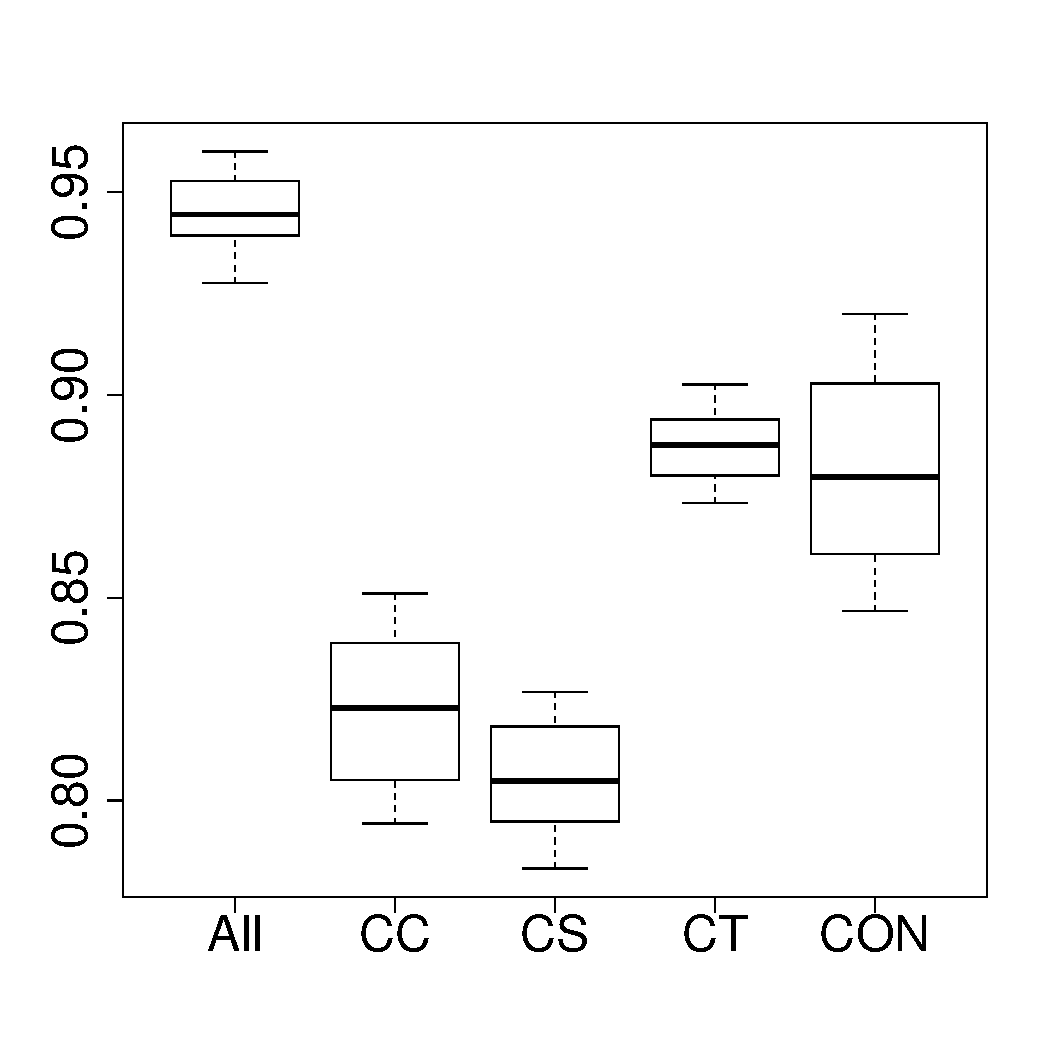
\includegraphics[width=\linewidth]{Figures/runtime-hadoopkeep-importance.pdf}
                \caption{Res. time}
        \end{subfigure}%
        \begin{subfigure}{0.19\textwidth}
                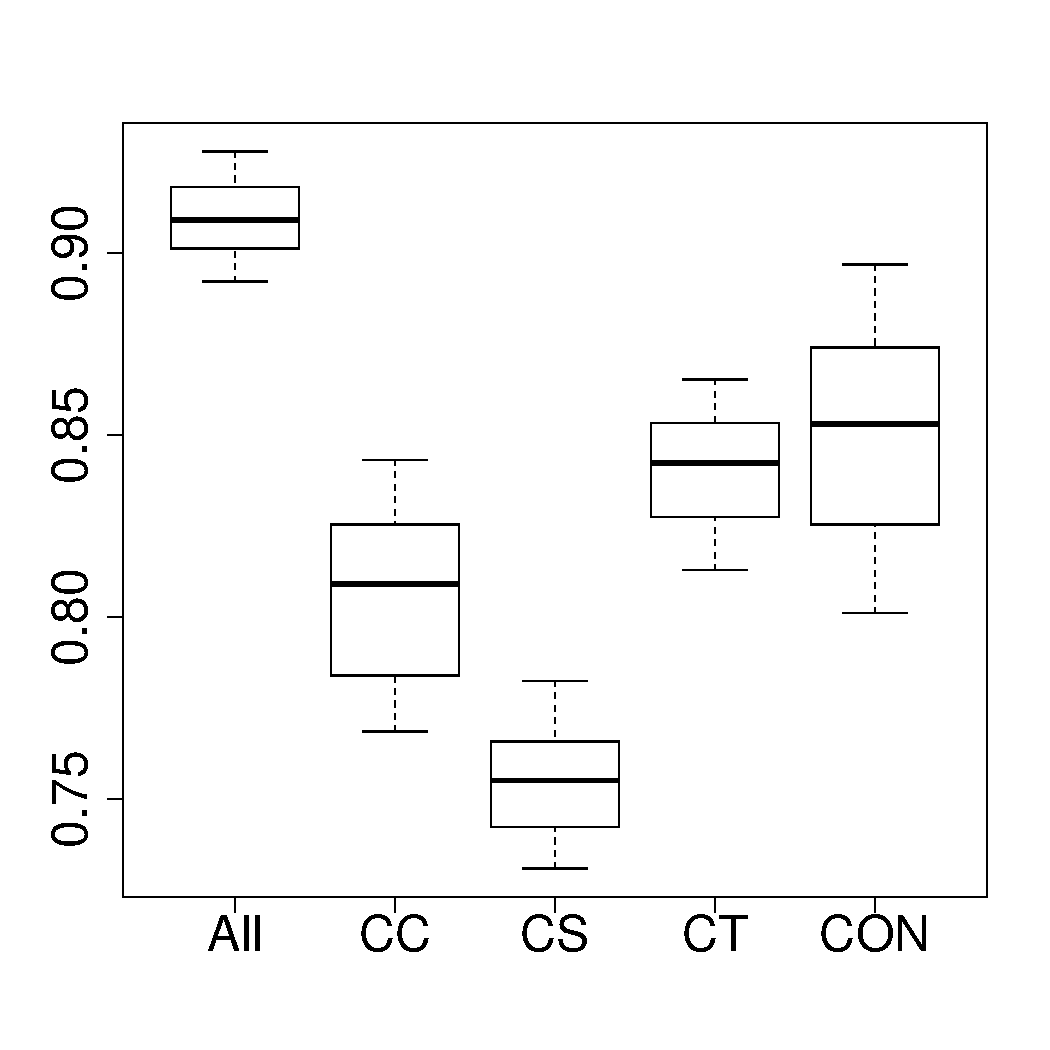
\includegraphics[width=\linewidth]{Figures/cpu-hadoopkeep-importance.pdf}
                \caption{CPU}
        \end{subfigure}%
        \begin{subfigure}{0.19\textwidth}
                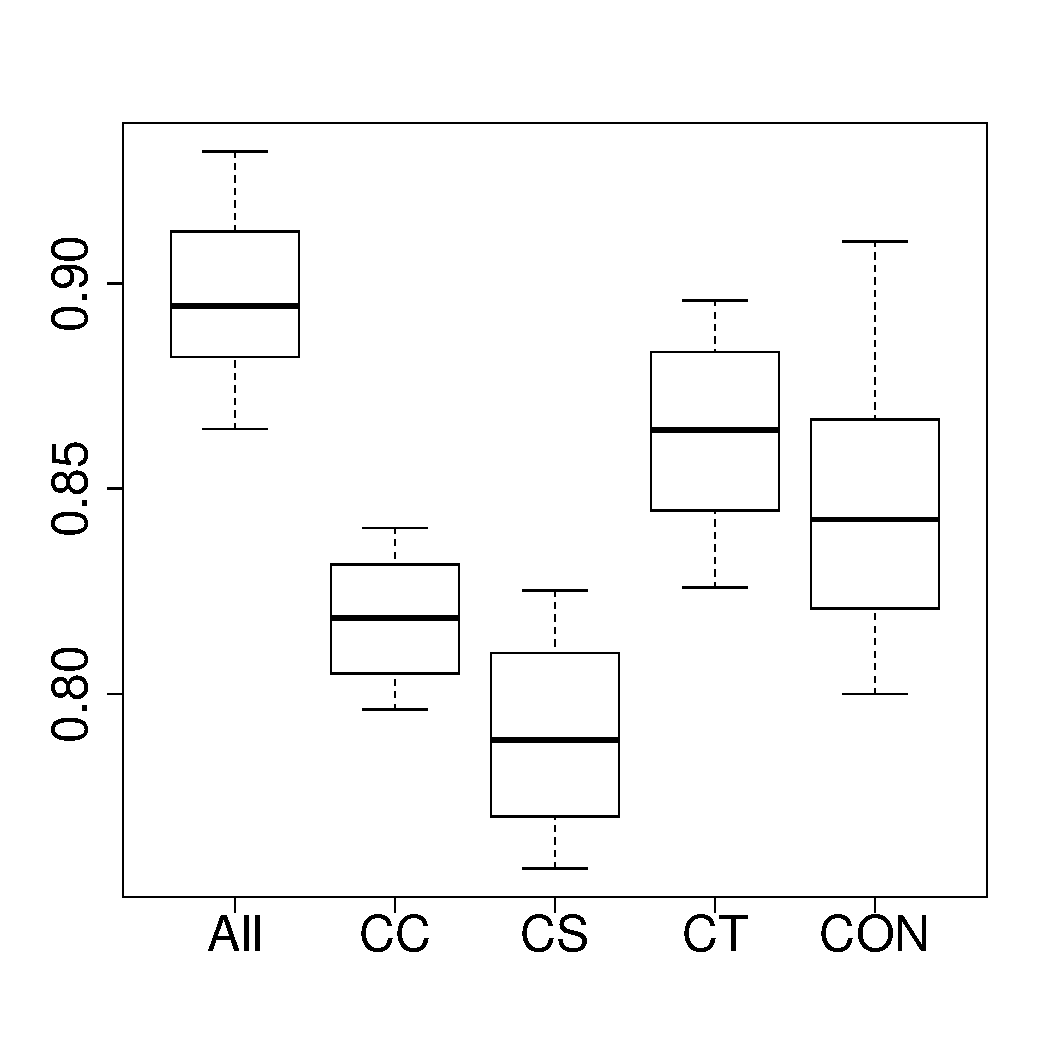
\includegraphics[width=\linewidth]{Figures/mem-hadoopkeep-importance.pdf}
                \caption{Memory}
        \end{subfigure}%
        \begin{subfigure}{0.19\textwidth}
                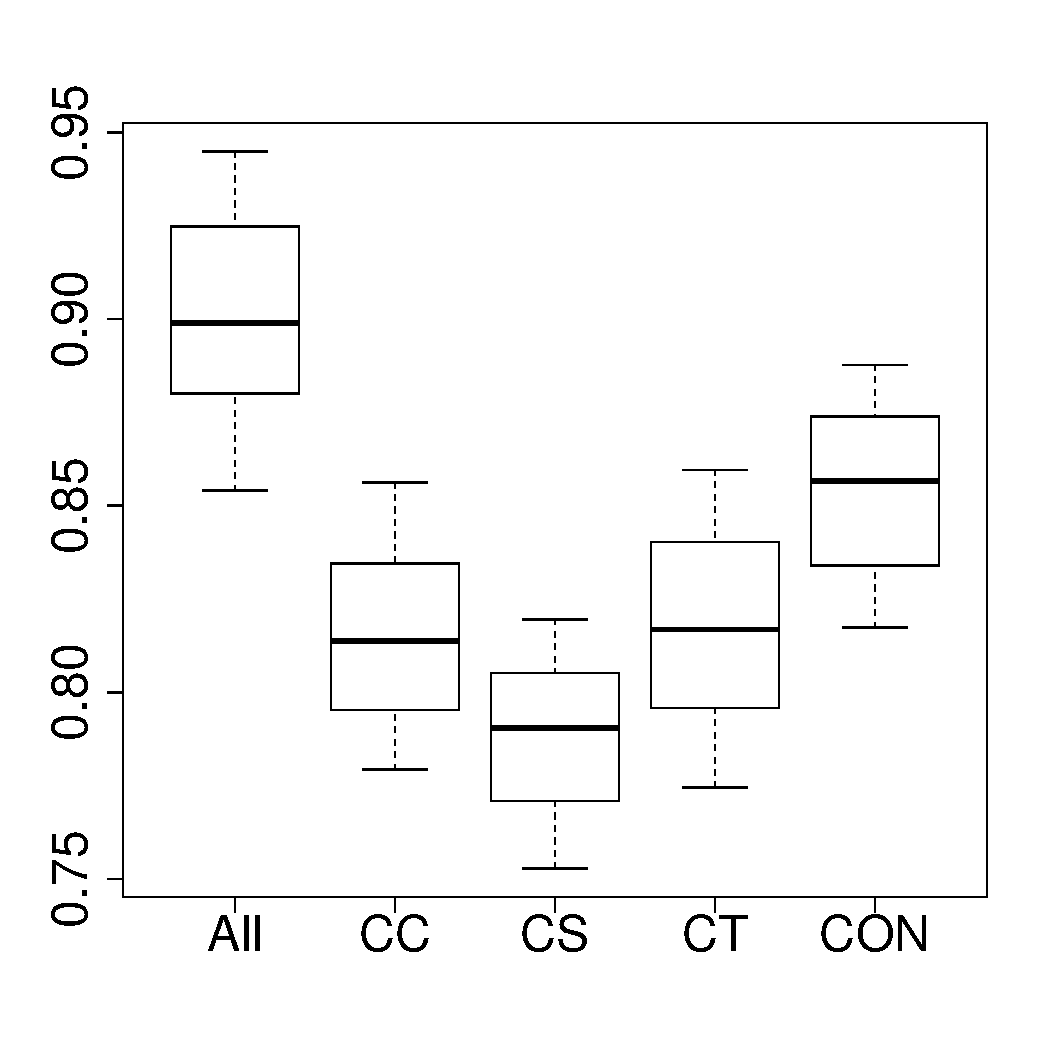
\includegraphics[width=\linewidth]{Figures/ioread-hadoopkeep-importance.pdf}
                \caption{I/O read}
        \end{subfigure}
        \begin{subfigure}{0.19\textwidth}
                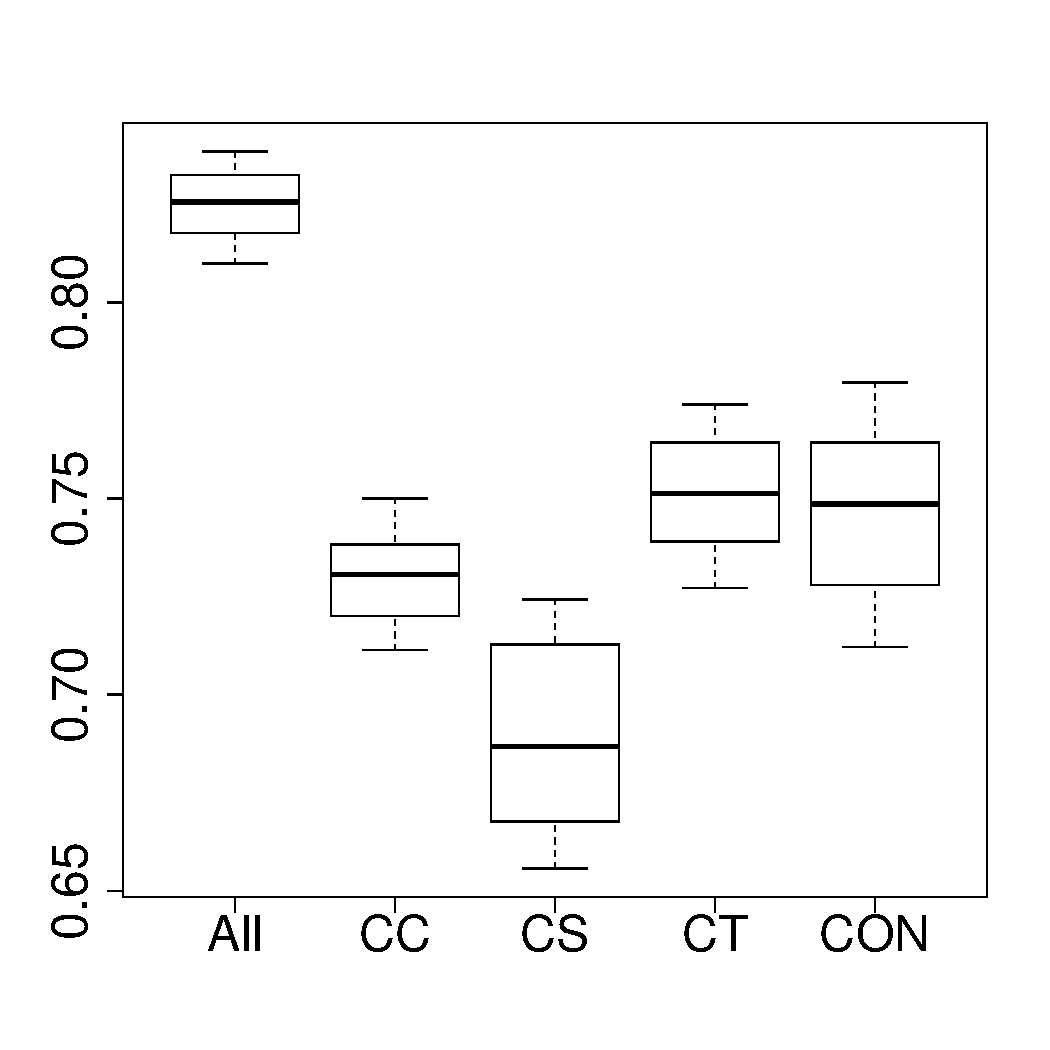
\includegraphics[width=\linewidth]{Figures/iowrite-hadoopkeep-importance.pdf}
                \caption{I/O write}
        \end{subfigure}
        
	\caption{AUC of RF for \emph{Hadoop} when only keeping one dimension of metrics.}
	\label{fig:importance-dimenssion-keep-hadoop}
\end{figure}

\begin{figure}[t]
	\centering
        \begin{subfigure}{0.19\textwidth}
                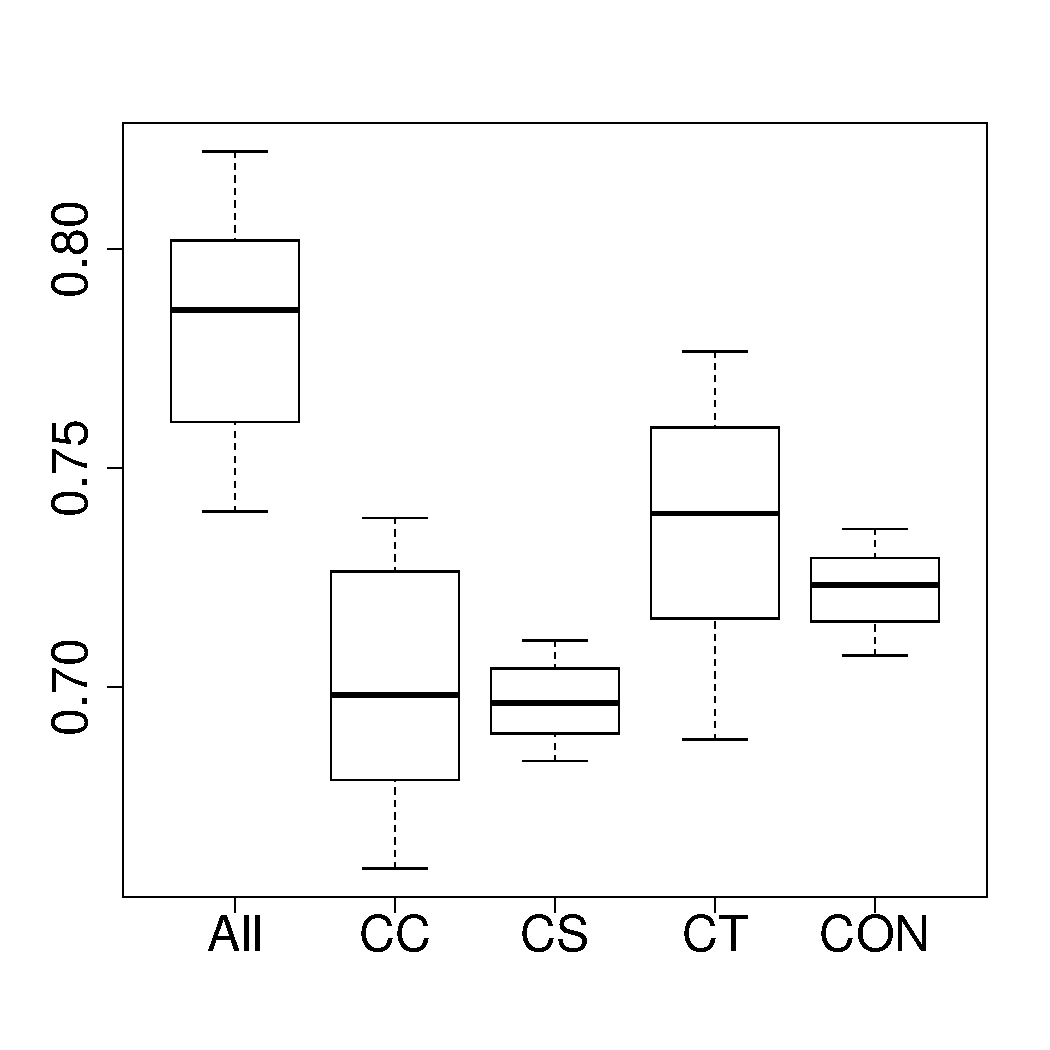
\includegraphics[width=\linewidth]{Figures/runtime-cassandrakeep-importance.pdf}
                \caption{Res. time}
        \end{subfigure}%
        \begin{subfigure}{0.19\textwidth}
                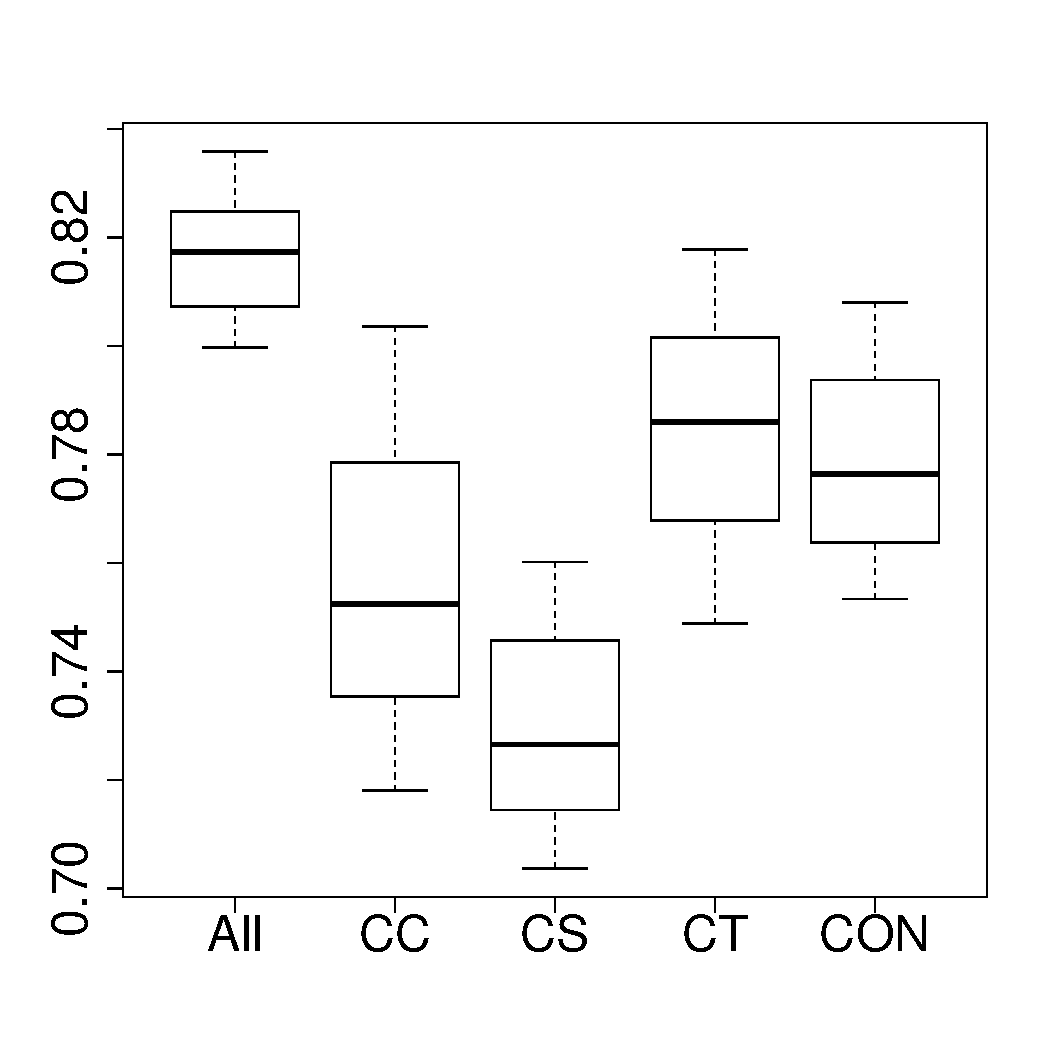
\includegraphics[width=\linewidth]{Figures/cpu-cassandrakeep-importance.pdf}
                \caption{CPU}
        \end{subfigure}%
        \begin{subfigure}{0.19\textwidth}
                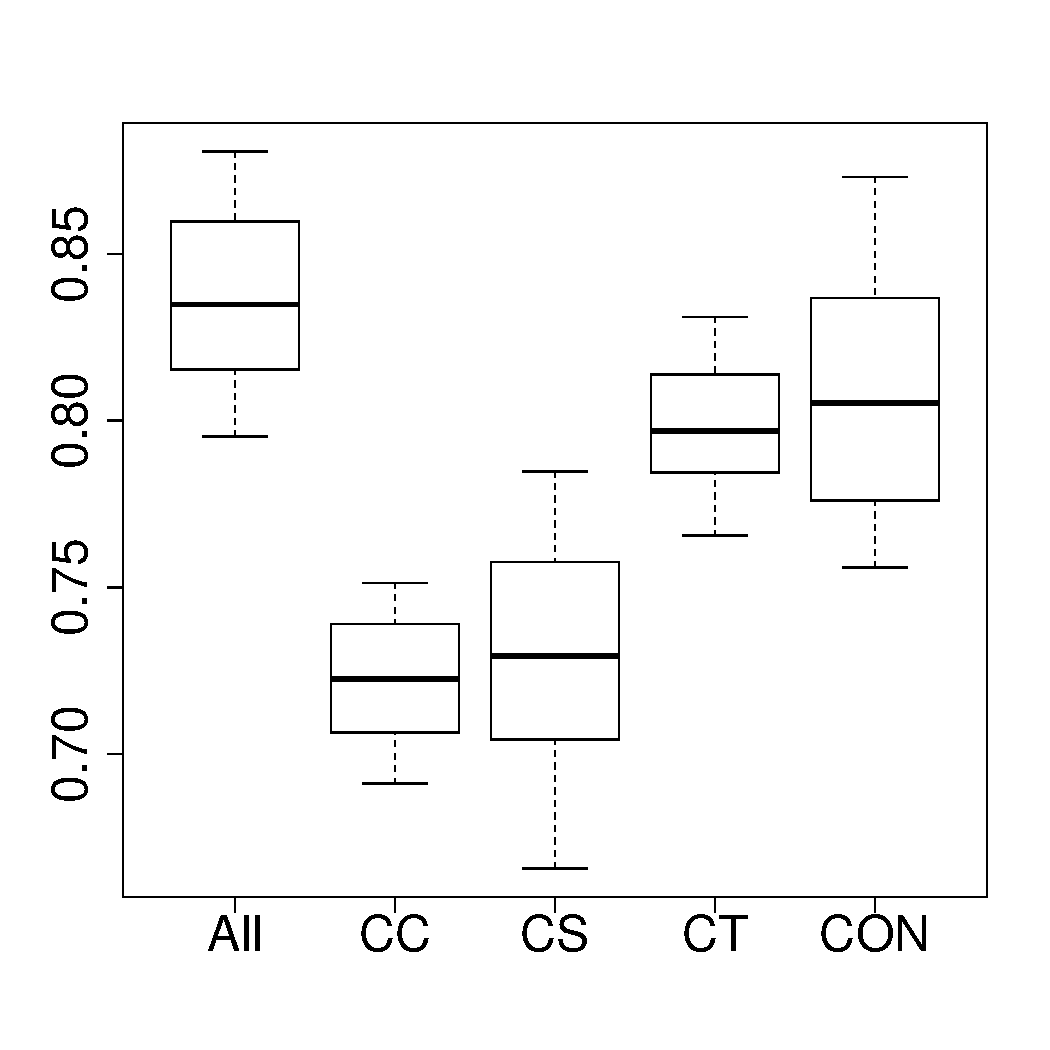
\includegraphics[width=\linewidth]{Figures/mem-cassandrakeep-importance.pdf}
                \caption{Memory}
        \end{subfigure}%
        \begin{subfigure}{0.19\textwidth}
                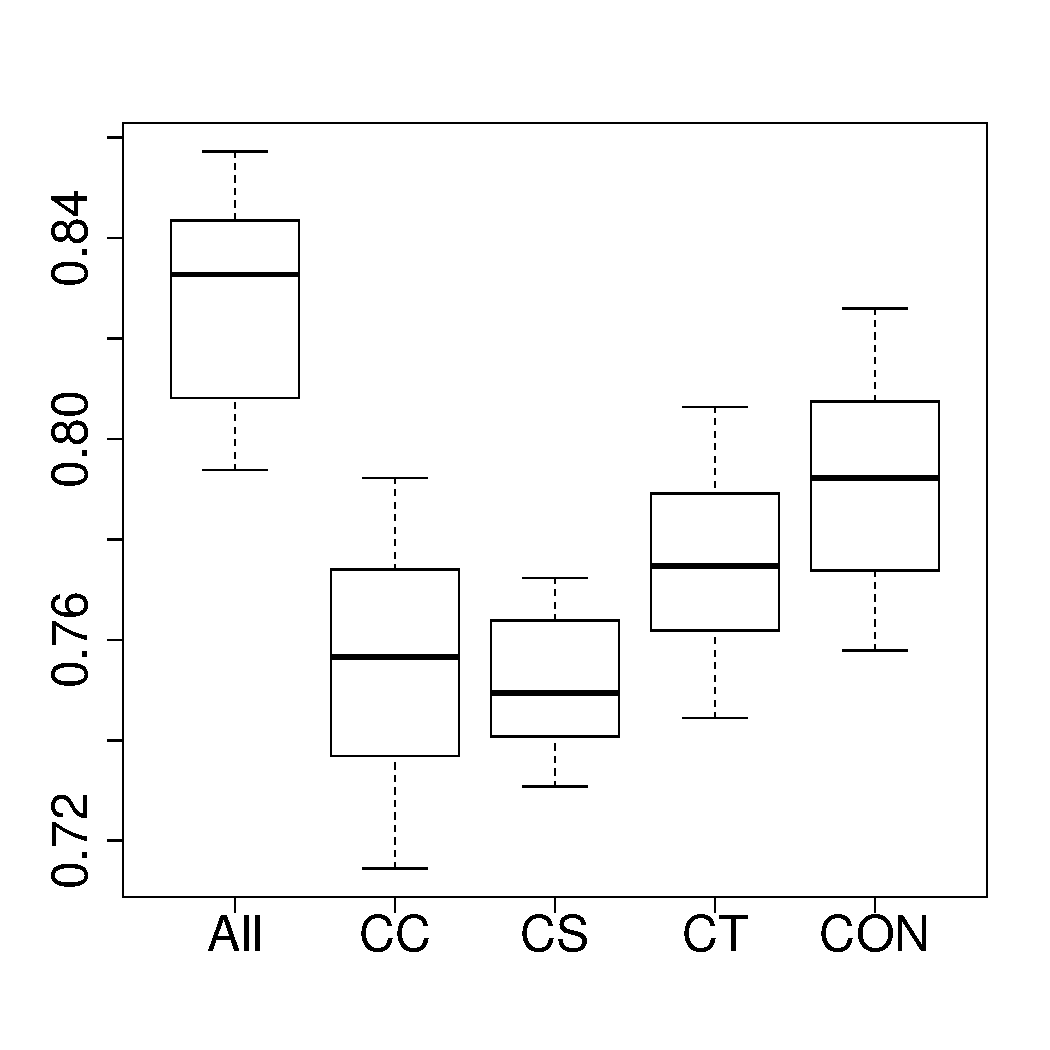
\includegraphics[width=\linewidth]{Figures/ioread-cassandrakeep-importance.pdf}
                \caption{I/O read}
        \end{subfigure}
        \begin{subfigure}{0.19\textwidth}
                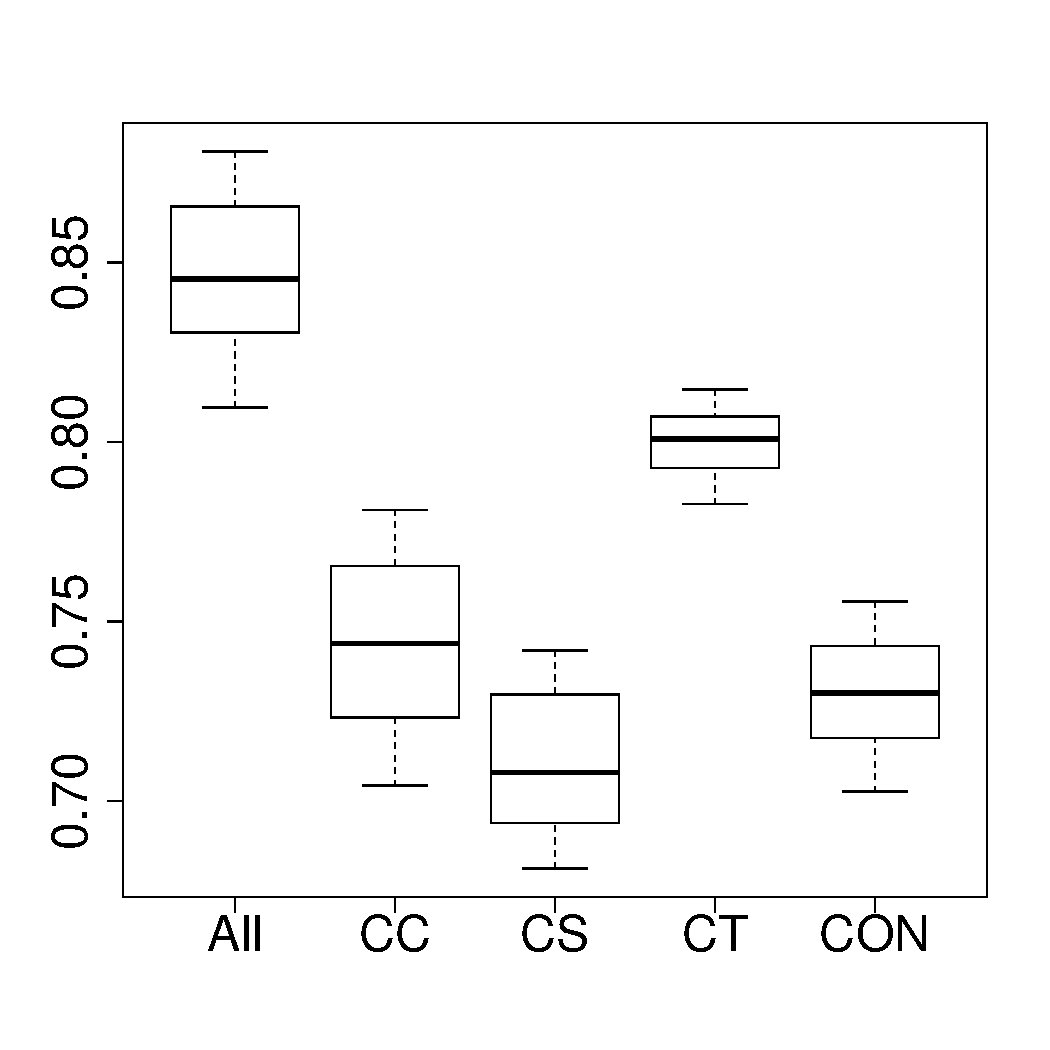
\includegraphics[width=\linewidth]{Figures/iowrite-cassandrakeep-importance.pdf}
                \caption{I/O write}
        \end{subfigure}
        
	\caption{AUC of RF for \emph{Cassandra} when only keeping one dimension of metrics.}
	\label{fig:importance-dimenssion-keep-cassandra}
\end{figure}

\begin{figure}[t]
	\centering
        \begin{subfigure}{0.19\textwidth}
                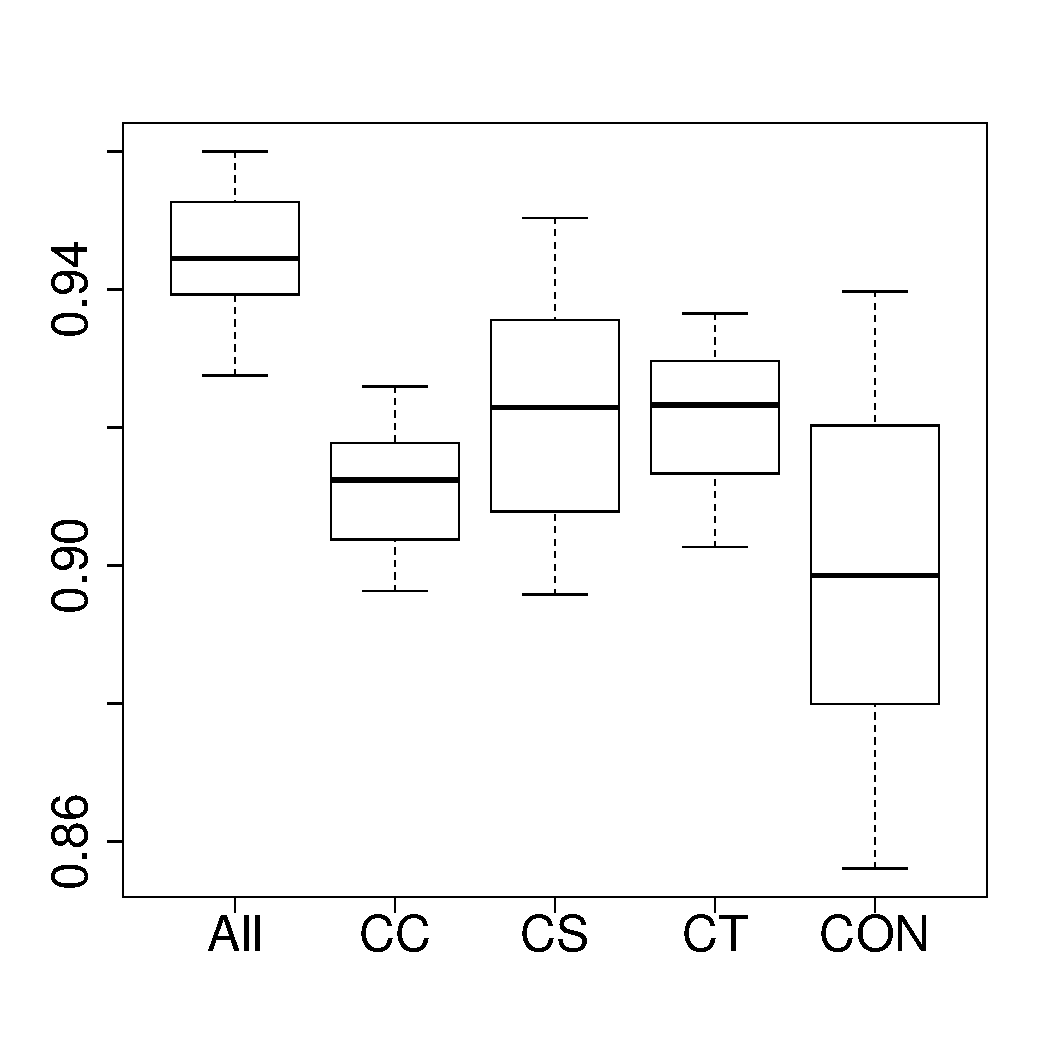
\includegraphics[width=\linewidth]{Figures/runtime-hadoopremove-importance.pdf}
                \caption{Res. time}
        \end{subfigure}%
        \begin{subfigure}{0.19\textwidth}
                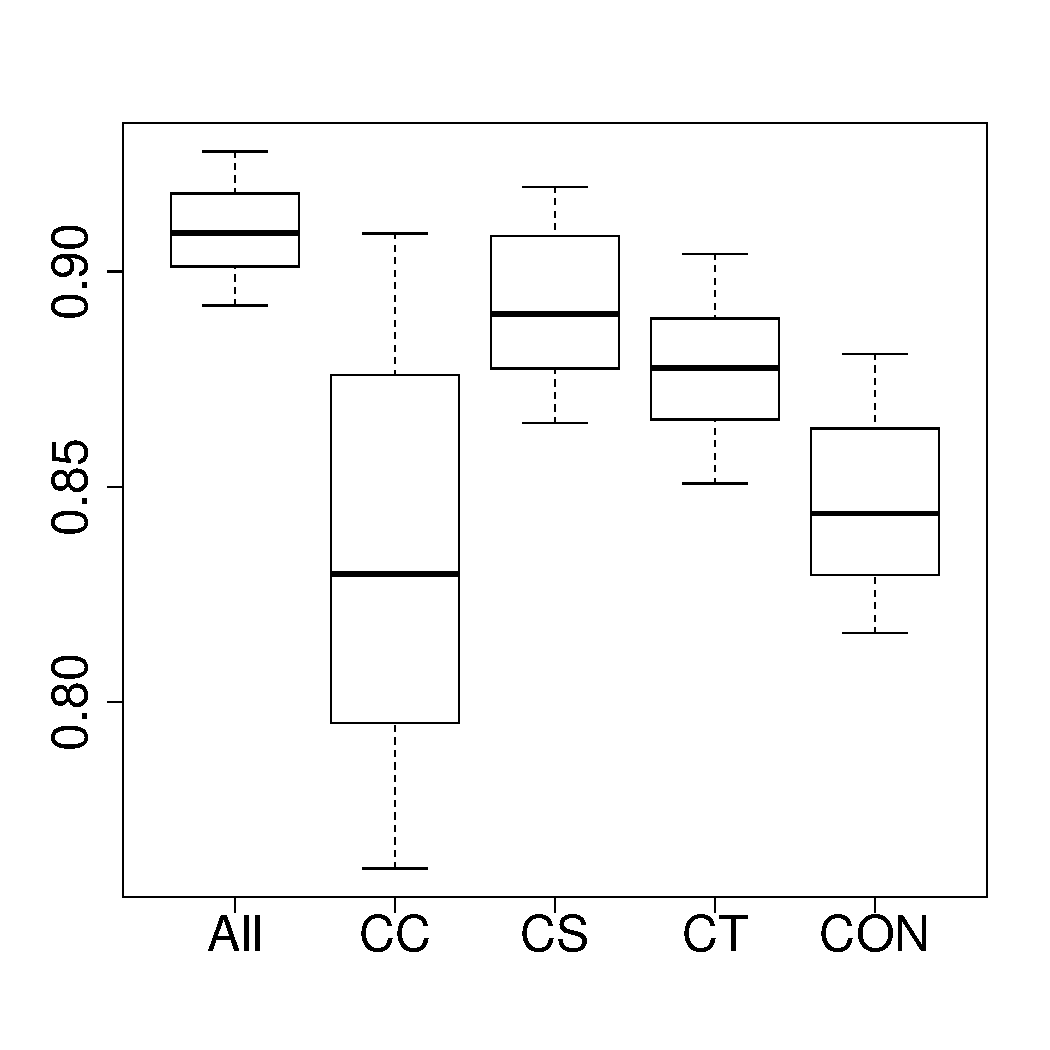
\includegraphics[width=\linewidth]{Figures/cpu-hadoopremove-importance.pdf}
                \caption{CPU}
        \end{subfigure}%
        \begin{subfigure}{0.19\textwidth}
                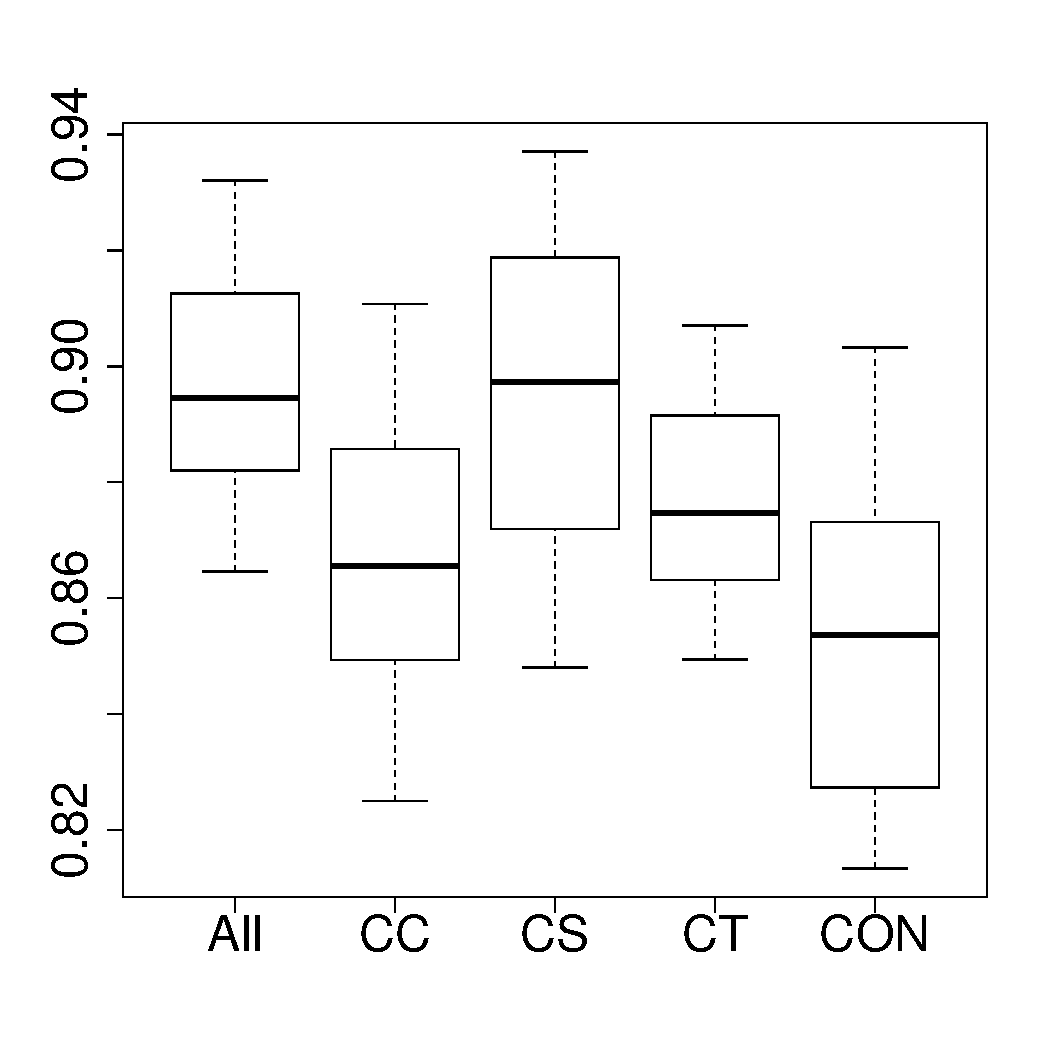
\includegraphics[width=\linewidth]{Figures/mem-hadoopremove-importance.pdf}
                \caption{Memory}
        \end{subfigure}%
        \begin{subfigure}{0.19\textwidth}
                \includegraphics[width=\linewidth]{Figures/ioread-hadoopremove-importance.pdf}
                \caption{I/O read}
        \end{subfigure}
        \begin{subfigure}{0.19\textwidth}
                \includegraphics[width=\linewidth]{Figures/iowrite-hadoopremove-importance.pdf}
                \caption{I/O write}
        \end{subfigure}
        
	\caption{AUC of RF for \emph{Hadoop} when removing one dimension of metrics.}
	\label{fig:importance-dimenssion-remove-hadoop}
\end{figure}

\begin{figure}[t]
	\centering
        \begin{subfigure}{0.19\textwidth}
                \includegraphics[width=\linewidth]{Figures/runtime-cassandraremove-importance.pdf}
                \caption{Res. time}
        \end{subfigure}%
        \begin{subfigure}{0.19\textwidth}
                \includegraphics[width=\linewidth]{Figures/cpu-cassandraremove-importance.pdf}
                \caption{CPU}
        \end{subfigure}%
        \begin{subfigure}{0.19\textwidth}
                \includegraphics[width=\linewidth]{Figures/mem-cassandraremove-importance.pdf}
                \caption{Memory}
        \end{subfigure}%
        \begin{subfigure}{0.19\textwidth}
                \includegraphics[width=\linewidth]{Figures/ioread-cassandraremove-importance.pdf}
                \caption{I/O read}
        \end{subfigure}
        \begin{subfigure}{0.19\textwidth}
                \includegraphics[width=\linewidth]{Figures/iowrite-cassandraremove-importance.pdf}
                \caption{I/O write}
        \end{subfigure}
        
	\caption{AUC of RF for \emph{Cassandra} when removing one dimension of metrics.} %\heng{the last box-plots have no label.} \heng{Make all the x/y labels bigger}}
	\label{fig:importance-dimenssion-remove-cassandra}
\end{figure}

%\noindent\textbf{All dimensions of metrics play important roles in our models, while the metrics may have different influence for different performance metrics and subject systems. } \heng{Test the significance of the difference between the models using all metrics and the models excluding one dimension of metrics. Alternative: use SK to rank the dimensions, including all metrics.}

%\noindent \textbf{\jinfu{Configuration and code token dimensions of metrics play more important roles in our model.}} The result of average AUC and AUC changes after removing each dimension of metrics is shown in Table~\ref{tab:dimension_importance}. 
%The results show that after removing each dimension of metrics, the AUC values decreases ranging from 0.02 to 0.09. The results of only keeping one dimension metrics is shown in Table~\ref{tab:one_dimension_importance}. The values of average AUC changes ranging from 0.04 to 0.14. Intuitively, the most important dimension metrics are the metrics from configuration dimension. %In particular, for \emph{Hadoop}, the average AUC value in configuration dimension decreases by 0.06 compared to the original model. The second most important dimension metrics is code change dimension metrics. 

%To examine whether there exist statistically significantly difference in AUC between original model and the resulting model, we apply e Mann-Whitney U test on our resulting AUC data. The result is shown in Table~\ref{tab:difference}. The results show that there exist statistically significant difference (p\_value  \textless  0.05) in the predictions between most of the dimension metrics and all metrics. Such results imply that any of dimension metrics play important roles in our models.



\begin{comment}

\med{to remove with table 10}\noindent\textbf{For the Hadoop project, the \textit{configuration option} dimension has the most top-ranked metrics; while for the Cassandra project, the \textit{code change} and \textit{code token} dimensions have the most top-ranked metrics.}
\med{not sure to understand this ->}As discussed in RQ1, the configuration options show more consistent influence on the performance regression detection in the Hadoop project than in the Cassandra project, which could explain that the configuration metrics are ranked higher in the Hadoop project. 
%\heng{Detailed examples of individual metrics and their meanings.}
The results of average rank of the top important individual metrics is shown in Table~\ref{tab:individual_importance}. For \emph{Hadoop}, the results show that the most important metric is the token named \emph{groups} in dimension configuration. For \emph{Cassandra}, the most important metric is \emph{Entropy} in dimension code change. 

\begin{table}
\tabcolsep=0.05cm
\tiny
\caption{Average rank of the top ten important metrics and their corresponding dimension.}

\begin{tabular}{|c|c|c|c|c|c|c|c|c|c|c|}
\hline
\multicolumn{11}{|c|}{Hadoop}                                                                                                                                                    \\ \hline
\multirow{2}{*}{Rank} & \multicolumn{2}{c|}{Res. Time} & \multicolumn{2}{c|}{CPU} & \multicolumn{2}{c|}{Memory} & \multicolumn{2}{c|}{I/O read} & \multicolumn{2}{c|}{I/O write} \\ \cline{2-11} 
                      & dimension    & metric          & dimension  & metric      & dimension      & metric     & dimension   & metric          & dimension    & metric          \\ \hline
1                     & config       & groups          & config     & groups      & Change    & Entropy    & config      & stream          & config       & groups          \\ \hline
2                     & config       & multipart       & config     & secs        & config         & groups     & Change      & Entropy         & config       & idlethreshold   \\ \hline
3                     & Change       & Entropy         & config     & after       & config         & stream     & config      & after           & config       & ipc             \\ \hline
4                     & config       & ipc             & config     & kill        & config         & secs       & config      & symlinks        & config       & after           \\ \hline
5                     & config       & zk              & Change     & Entropy     & config         & checksum   & config      & groups          & Change       & Entropy         \\ \hline
6                     & config       & secs            & config     & close       & token          & static     & config      & ipc             & config       & retries         \\ \hline
7                     & config       & authorization   & config     & checksum    & config         & symlinks   & config      & secs            & config       & secs            \\ \hline
8                     & token        & build           & config     & symlinks    & config         & after      & config      & authorization   & config       & checksum        \\ \hline
9                     & config       & checksum        & config     & stream      & config         & server     & config      & close           & config       & stream          \\ \hline
10                    & token        & builtin         & config     & tcpnodelay  & config         & kill       & config      & maxidletime     & config       & symlinks        \\ \hline
\multicolumn{11}{|c|}{Cassandra}                                                                                                                                                 \\ \hline
\multirow{2}{*}{Rank} & \multicolumn{2}{c|}{Res. Time} & \multicolumn{2}{c|}{CPU} & \multicolumn{2}{c|}{Memory} & \multicolumn{2}{c|}{I/O read} & \multicolumn{2}{c|}{I/O write} \\ \cline{2-11} 
                      & dimension    & metric          & dimension  & metric      & dimension      & metric     & dimension   & metric          & dimension    & metric          \\ \hline
1                     & Change       & Entropy         & Change     & Entropy     & Change         & Entropy    & Change      & Entropy         & Change       & Entropy         \\ \hline
2                     & Structure    & Fanin           & Structure  & Fanin       & Structure      & Fanin      & Structure   & Fanin           & Structure    & Fanin           \\ \hline
3                     & Change       & SOCM            & Change     & NS          & Change         & NS         & Change      & NS              & token        & cql             \\ \hline
4                     & token        & cql             & Change     & SOCM        & Change         & SOCM       & token       & get             & Change       & NS              \\ \hline
5                     & Change       & NS              & token      & metadata    & token          & get        & Change      & SOCM            & Change       & SOCM            \\ \hline
6                     & token        & get             & token      & equal       & token          & t          & token       & metadata        & token        & get             \\ \hline
7                     & Change       & SUMC            & token      & get         & token          & metadata   & token       & kei             & Change       & SUMC            \\ \hline
8                     & token        & metadata        & token      & kei         & token          & equal      & Change      & SUMC            & token        & metadata        \\ \hline
9                     & config       & failure         & Change     & SUMC        & token          & kei        & token       & in              & token        & d               \\ \hline
10                    & token        & kei             & config     & failure     & token          & size       & token       & store           & token        & kei             \\ \hline
\end{tabular}

\label{tab:individual_importance}
\end{table}


\end{comment}


\vspace{0.5cm}
\begin{Summary}{Summary of RQ2}{}
Every dimension of metrics plays an statistically significant role in predicting whether a \instance manifests a \inconsistent problem. The most important dimensions are related to code tokens and configurations. 
\end{Summary}


\section{Threats to Validity}
\label{sec:threats}
In this section, we discuss the threats to the validity of our study. 

\noindent \textbf{External validity.} The first external threat to validity concerns the generalizability of our results to other software systems. Due to the expensive computing resources needed (we spent around 12,536 machine hours collecting performance data), we conducted our evaluation on two open-source software systems, i.e., \emph{Hadoop} and \emph{Cassandra}. Our findings may not generalize to other software systems. %Our evaluated software systems are implemented in \emph{Java}. Therefore, our findings might not be generalizable to software systems implemented in other programming languages.
However, we found motivating results on the prevalence of \inconsistent and the performance of our explanatory model, which can be replicated by future studies on other software systems. % can evaluate our approach and findings on commercial software systems with other languages. 

\noindent \textbf{Internal validity.}
When we collect our commits data, We only consider the last commit, if multiple commits are associated with the same issue. We may miss some commit with code change. Future work can study the difference if considering all the commits.

Another internal threat to validity concerns the performance metrics that we consider. In our approach, we collect five popular performance metrics, i.e., Response time, CPU, Memory, I/O read and write, while other performance metrics such as throughput can still be explored by future research.% can choose other performance metrics to complement our study. 


Similarly, our explanatory model does not cover all the possible dimensions of metrics. For example, we do not consider a developer dimension. However, our model shows a good AUC performance to predict whether a \instance manifests an \inconsistent. Future studies can explore more dimensions of metrics to improve the performance of our models. 

Finally, our evaluation considers just the traditional models (i.e., logistic regression, random forest, and XGBoost) and neural network models (i.e., general neural network and convolutional neural network). Although we do not cover all existing models, our study covers the most popular ones that are used in software engineering. Future work is encouraged to explore more models. 


%In RQ2, we use four dimension metrics, i.e., code change, code structure, code token, and configuration option to build our prediction model. However, there exist other dimension metrics such as metrics from developer.  

%We choose three traditional models, i.e., logistic regression, random forest, and XGBoost and two neural network models, i.e., general neural network and convolutional neural network to construct our predictors. There are more machine learning algorithms can be used to build our model. Future research can add more metrics and use other machine learning algorithms to improve the results.

\noindent \textbf{Construct validity.} %Our evaluation is based on the stability and correctness of collected performance data. The quality and correctness of recorded performance data can impact our study. We assume that the performance monitoring tool named \emph{psutil} can accurately capture performance metrics. \emph{psutil} has been widely used in software performance study~\cite{DBLP:conf/icsm/AlghmadiSSH16, DBLP:conf/icsm/ChenS17}. 
There might exist environmental performance noise when we use \emph{psutil} to capture the performance data. To minimize the noise, we capture the performance of the corresponding Linux process of the running tests. Furthermore, for each test, we repeat the execution 30 times independently. %\med{is this correct?}
Finally, we run all of our experiments in the same environments. %\bram{what does ``configuration'' mean here?}.

\section{Related Work}
\label{sec:relatedwork}

In this section, we discuss prior work along two dimensions: software configuration and software performance. % engineering.

\subsection{Software Configuration}

A large body of research efforts have been conducted on software configuration, which mainly focus on understanding configuration problems, preventing configuration errors, and debugging configuration errors. Few research efforts consider the performance aspect of software configuration \bram{wasn't there a lot of work on performance tuning in Mohammed's TSE survey?}. 

\subsubsection{Understanding Configuration Problems}
Configuration makes a software system complex~\cite{tse}, which leads to configuration errors that are severe, common, and hard to debug~\cite{RN3251}. For instance, Jin et al.~\cite{RN2897} found that configuration options add more complexity to the development and testing of highly configurable software systems. Han et al.~\cite{RN2864} found that configuration options are responsible for 59\% of the performance bugs. Gousios et al.~\cite{RN3551} observed that the configuration of the garbage collectors have an impact on the performance of server applications. Furthermore, Sayagh et al.~\cite{RN3249, RN2758} found that the impact of a configuration option can spread to multiple layers of an architectural stack.% Jin et al.~\cite{RN2897} found that there is a need for tools that debug configuration errors in multi-languages software systems. 

%Our work is different from this line of research as we consider the performance regression that is caused by configuration options.
%\subsubsection{Debugging Configuration Errors} 
A second line of research proposed and evaluated different approaches to identify misconfigured configuration options. Dong et al.\cite{RN2805, RN3163} leverage the slicing technique to identify the misconfigured option for a given error message or exception. Rabkin et al.~\cite{RN2822} leverage a data flow analysis technique to identify for each option, which source code lines it might impacts. Attaryian et al.~\cite{RN3248} combined dynamic control and data flow analysis to identify misconfigured options. Zhang et al.~\cite{RN2839, RN2777} compared the trace of a correct execution against the trace of an incorrect execution to identify culprit options. We refer to our prior systematic literature review~\cite{tse} and the work of Tianyin et al.~\cite{RN3252} and Andrzejak et al.\cite{andrzejaksoftware} for further details about the existing configuration debugging approaches. 

Our work is different from this line of research since we do not consider debugging configuration errors, but understanding and identifying performance regressions that are caused under certain configurations.

\subsubsection{The Performance of Configurations} 

Another line of research considers the identification of the optimal configurations for a software system and the debugging of performance errors that are caused by configuration options. Attariyan et al.~\cite{RN3253} proposed an approach based on dynamic taint analysis technique to identify the option that causes a performance error. % assigns to each source code block a cost, use a dynamic analysis techniques that instruments and runs a software system, then their approach identifies which blocks were executed and which options they depends on. 
Siegmund et al.~\cite{RN2880} build mathematical models that describe the impact of a configuration on software performance based on each option's value. Raghavachari et al.~\cite{RN3537} proposed an iterative approach to identify an optimal configuration in terms of performance. Their approach consists of selecting for a J2EE web application a first configuration, compare its performance to a second configuration until the optimal configuration is found. Similarly, Dia et al.~\cite{RN3543} proposed an approach that automatically adjusts the values of existing configuration options at run-time to optimize the CPU and memory usage objectives.

Li et al.~\cite{LiAutoConfig} leveraged performance monitoring data and execution logs to dynamically optimize the values of performance-related configuration options according to varying workloads in the field. Guo et al.~\cite{RN3544} leverage non-linear regression to suggest an optimal configuration. However, collecting a large amount of data for training a model that predicts the performance of a configuration is expensive. Therefore, Sarkar et al.~\cite{RN3089} evaluated the progressive and projective sampling to train a model that predicts the performance of configuration. For their initial training sample, they consider data on which each option is enabled at least once. Other efforts identified the optimal configuration options in terms of performance by leveraging existing optimization approaches, i.e., iterative search~\cite{RN3545}, multi-objective optimization~\cite{singh2016optimizing}, and smart hill climbing~\cite{RN3518}.


The goal of our paper is not to identify optimal configuration options or to debug an existing performance-related configuration error. Instead, we focus on studying inconsistent option performance through different commits. In particular, we focus on understanding whether a performance improvement or regression is consistent through all the values of an option. That is important, as one can improve the performance of a software system or release new changes that do not impact the performance under one configuration when other configurations hide a performance regression. 

Furthermore, prior work on this line of research compares the absolute performance between two values for the same option, while this can be subjective, as discussed earlier. One option's value can naturally consume performance as it enables the execution of additional features. However, the execution of the software system under the same option's value can be improved \bram{for those features? flow in this paragraph is unclear} compared the same option and value prior to that commit. In addition, a better performing option's value can show a regression compared to the prior commit as well. %impact of configuration options on the performance regression.% While a new commit does not show any performance regression under the default configuration, other configurations might show a low performance when the same configuration showed a good performance in the prior commit. 

\subsection{Software Performance}

Performance is an important aspect of software quality. Extensive prior research has been conducted to study software performance. In this subsection, we summarize the empirical studies on  %performance to 
understanding software performance and the studies on %. We then present the related works of 
performance regression detection.

\subsubsection{Empirical Studies on Software Performance}
Several empirical studies have been conducted on the performance of software systems~\cite{ICSE2014:Huang,Jin:2012,MSR11:Zaman,MSR12:Zaman,DBLP:conf/kbse/HanYL18,Leitner2017ICPE}. For instance, Jin \emph{et al$.$}~\cite{Jin:2012} studied 109 real world performance issues that are reported from five open source software systems and %. Based on the studied 109 performance bugs, the authors 
%developed an automated tool 
proposed an approach to detect performance issues. Zaman \emph{et al$.$}~\cite{MSR11:Zaman,MSR12:Zaman} conducted qualitative and quantitative studies on performance issues. They found that developers and users face problems in reproducing performance bugs %. More time is 
as they spend % 
a lot of time on discussing performance bugs %than 
compared to other kinds of bugs (e.g., functional bugs). %\jinfu{For example, Firefox performance bugs take more time to discuss and fix.\med{I meant examples of other kinds of bugs}} 
Huang \emph{et al$.$}~\cite{ICSE2014:Huang} %studied real world performance issues. They 
proposed an approach to improve the efficiency of performance regression testing by leveraging a static analysis technique to estimate the risk of a given commit in introducing a performance regression. Han et al$.$~\cite{DBLP:conf/kbse/HanYL18} studied %y
300 bug reports from three large open source projects. The authors found that most of the performance bugs occur for specific combinations of data input and configurations. They also proposed a framework named \emph{PerfLearning} to extract such data input and configurations from bug reports to generate test frames. Leitner et al$.$~\cite{Leitner2017ICPE} %aim to understand the current state of art of performance testing. They conduct a study on 111 open-source java-based systems from GitHub 
investigated the state-of-the-practice related to performance tests. The authors found that performance tests form only a small portion of a test suite.
%and use a combination of quantitative and qualitative research methods to investigate the use of performance tests across five perspectives.

The vast amount of research on software performance signifies its importance and motivates our work. %Prior studies on performance typically are based on either limited performance issue reports or release of the software. 
Different from prior research, we evaluate software performance at the commit level and study performance regressions that are manifested under a subset of the possible configurations. % by configuration option.
In addition, our work is different from this line of research as we consider how to avoid performance regressions that are related to some configurations while being hidden by other configurations, instead of understanding the existing performance related issues. 

\subsubsection{Performance regression detection}
Extensive prior research has proposed automated techniques to detect performance regressions. Such detection techniques can be divided into two categories: measurement-based and model-based detection. 

Measurement-based approaches compare performance metrics (e.g., CPU usage) between two consecutive versions to detect performance regressions. %measure performance metrics and compares these performance metrics between two consecutive versions of a system to detect performance regression. 
For example, Nguyen \emph{et al$.$}~\cite{Nguyen:2012:ADP,nguyen2011automated,Nguyen:2014:ICS} %conducted a series of studies on performance regressions. Nguyen \emph{et al$.$} apply control charts to analyze performance counters across test runs to detect performance regression automatically. They construct the control chart to detect performance regressions  by setting upper and lower bounds of performance counters.
leveraged control charts to identify performance regressions. %~\heng{treat regression as a countable word throughout the paper, countable seems better}. 
A control chart has a upper control limit and a lower control limit. A performance regression is detected when a performance metric is above the upper limit or bellow the lower limit. Foo \emph{et al$.$}~\cite{foo2010mining} proposed an approach that compares a test's performance metrics to historical performance metrics. %\med{from what?}performance regression testing repositories to detect potential performance regressions. 

A model-based approach builds %\med{This paragraph is difficult to understand. What is detected model? is it prediction model? and what is counters? what is signatures? what do you mean by heterogeneous environment?} 
%\jinfu{detected model is a general model, we can use model. Performance counter is performance metric, like CPU usage. Some papers use signatures to represent system users' behavior.} \med{I updated this paragraph, though Bodik work is not clear} 
a machine learning model with a set of performance metrics to detect performance regressions.  
Cohen et al.~\cite{Cohen:2005:CIC} showed as implication that it is ineffective and not enough to index and identify performance problems with simple records of raw system metrics. Cohen et al. used TAN (Tree-Augmented Bayesian Network) models to model the system performance states based on a small subset of metrics. %Therefore, the authors present an approach to capture signatures representing system states from a running system and cluster such signitures to detect recurrent or similar performance problems. 
Bodik \emph{et al$.$}~\cite{bodik2008hilighter} leveraged a logistic regression model to model system users' behavior to improve Cohen \emph{et al$.$}\textquotesingle s model. %~\heng{need to mention Cohen's model beforehand}. 
Foo \emph{et al$.$}~\cite{DBLP:conf/icse/FooJAHZF15} proposed an approach that uses ensembles of models to detect performance regressions in heterogeneous environments (e.g., different hardware and software configurations). % \med{examples of what heterogeneous environments} \jinfu{different hardware and software configurations}). 
Xiong \emph{et al$.$}~\cite{Xiong:2013:VAM} proposed a model-driven framework to diagnose application performance and identify the root cause of performance issues. %Such framework uses linear regression to build the predict model to automatically diagnose the system performance in cloud environment and lead to root cause of performance problem.

%\med{well, we predict it, so it's kind of detecting performance regression}Our research is not designed to detect performance regression. The goal of our research is to examine the impact of configuration options on the performance regression. In our paper, we conduct measurement-based approach to identify performance regression on the commit level.

%\med{is the following paragraph correct?}
Our work complements this line of research in the sense that we consider the configuration aspect of highly configurable software systems. For instance, a code change might not show a performance regression on the default configuration, while leading to regressions on other configurations. This paper sheds light on the \inconsistent problem by first quantifying the existence of inconsistent performance variations, then proposing a prediction model that identifies the commits, tests, and options that exhibit the \inconsistent problem. 


\section{Conclusion}
\label{sec:conclusion}

Highly configurable software systems tend to have a large amount of existing options, which makes testing all possible configurations infeasible. That can, unfortunately, hide performance regression issues, which can go to the production as unseen. Furthermore, a developer might improve the performance of a software system, while the improvement might not be manifested when altering certain options' values. In fact, the performance improvement or regression of a software change might not be equally manifested through all the possible configuration options' values, which we refer to as the problem of Inconsistent Options Performance Variation (\inconsistent).

In this paper, %we first quantify the prevalence of such \inconsistent, and the difficulty to identify an option that manifests an \inconsistent. 
we observe that \inconsistent is a common problem, which is difficult to manually identify without running exhaustive tests, because most of the commits do not share similar options or tests that may lead to \inconsistent and hide performance regressions.
We also observed that predictive models (e.g., RF) can effectively predict the \inconsistent problems using four dimension of metrics that are related to code changes, code structures, code tokens, and configurations. 
Our findings highlight the importance of considering different configurations when performing performance regression detection, and that leveraging predictive models can mitigate the difficulty of exhaustively considering all configurations of a system during such a process. 
We expect that our study inspires a wide spectrum of future studies on configuration-aware performance regression detection.
%For instance, we observe that 81\% of the commits suffer from at least one option that suffers from the \inconsistent problem. 
%We also observe that most of the commits do not share similar options or tests that may lead to \inconsistent and hide performance regressions. %, and when they do so, the same options show different manifestations for \inconsistent (a few commits show an \inconsistent for that option, while other commits does not). 

%In this paper, we first quantify the regression that can be caused by the configuration options of a software system. Secondly, we propose a machine learning model to predict commits with a regression hidden with a configuration. 

%For instance, we observe that 69\% and 93\% of the Hadoop and Cassandra commits have at least one option with a performance regression (i.e., the performance of the current revision is statistically significantly different from the prior revision). Such regression issues have impact on different performance metrics, including the response time, CPU, memory, I/O read, and I/O write. 

%We then proposed and evaluated different prediction models to identify the \inconsistent issues. Our models use code change, code structure, code tokens, and configuration related metrics as independent metrics to predict \inconsistent based on five performance metrics (i.e., Response time, CPU, memory, I/O read, and I/O write). We observe that our models reach an AUC up to 0.94 for Hadoop and 0.90 for Cassandra. The most important metrics for our prediction are related to the code tokens and configuration dimensions. 




\bibliographystyle{IEEEtran}
\bibliography{ConfigSLR}


\end{document}
